\documentclass[11pt]{report}
\setcounter{tocdepth}{3}
\setcounter{secnumdepth}{3}
\usepackage[english, german]{babel}
\usepackage{geometry}                % See geometry.pdf to learn the layout options. There are lots.
\geometry{a4paper}                   % ... or a4paper or a5paper or ... 
%\usepackage[parfill]{parskip}    % Activate to begin paragraphs with an empty line rather than an indent
\usepackage{xifthen}
\usepackage{xstring}			% to check content of strings in xifthen
\usepackage{graphicx}
\usepackage[usenames,dvipsnames,table]{xcolor}
\usepackage{amssymb}
\usepackage{epstopdf}
\usepackage[utf8]{inputenc}
\usepackage{hyperref}
\usepackage{fancyhdr}
%\usepackage{natbib}
\usepackage{url}
\usepackage{float}
\usepackage{listings}
\usepackage{subfigure}

\usepackage[dvipsnames]{xcolor}
\usepackage{listings}

\lstdefinelanguage{Kotlin}{
  comment=[l]{//},
  commentstyle={\color{gray}\ttfamily},
  emph={delegate, filter, first, firstOrNull, forEach, lazy, map, mapNotNull, println, return@},
  emphstyle={\color{OrangeRed}},
  identifierstyle=\color{black},
  keywords={abstract, actual, as, as?, break, by, class, companion, continue, data, do, dynamic, else, enum, expect, false, final, for, fun, get, if, import, in, interface, internal, is, null, object, override, package, private, public, return, set, super, suspend, this, throw, true, try, typealias, val, var, vararg, when, where, while},
  keywordstyle={\color{NavyBlue}\bfseries},
  morecomment=[s]{/*}{*/},
  morestring=[b]",
  morestring=[s]{"""*}{*"""},
  ndkeywords={@Deprecated, @JvmField, @JvmName, @JvmOverloads, @JvmStatic, @JvmSynthetic, Array, Byte, Double, Float, Int, Integer, Iterable, Long, Runnable, Short, String},
  ndkeywordstyle={\color{BurntOrange}\bfseries},
  sensitive=true,
  stringstyle={\color{ForestGreen}\ttfamily},
}


\newcommand{\titleofthesis}{AKKalytics}
\newcommand{\department}{Informatik} % Replace by your department

\newcommand{\firstauthor}{Felix Kronsteinerr}
\newcommand{\firstauthorclass}{5AHIF}
\newcommand{\secondauthor}{Adzamija Alen}
\newcommand{\secondauthorclass}{5AHIF}
\newcommand{\thirdauthor}{Klatzer Emanuel}
\newcommand{\thirdauthorclass}{5AHIF}

\newcommand{\duedateen}{April 4, 2018} % due date in english format
\newcommand{\duedatede}{4. April 2018} % due date in german format
\newcommand{\supervisor}{Gerhard Aistleitner}
\newcommand{\projectpartner}{MIC}
 % Set basic data (author, title, etc.) of your thesis
\IfStrEq*{\languagename}{english}
	{
		\newcommand{\dalabel}{Diploma Thesis}
		\newcommand{\submittedlabel}{Submitted by}
		\newcommand{\datelabel}{Date}
		\newcommand{\duedatevalue}{\duedateen}
		\newcommand{\supervisorlabel}{Supervisor}
		\newcommand{\projectpartnerlabel}{Project Partner}
	}
	{
		\newcommand{\dalabel}{Diplomarbeit}
		\newcommand{\submittedlabel}{Eingereicht von}
		\newcommand{\datelabel}{Datum}
		\newcommand{\duedatevalue}{\duedatede}
		\newcommand{\supervisorlabel}{Betreuer}
		\newcommand{\projectpartnerlabel}{Projektpartner}
	}
 % This file should not really be touched

\begin{document}
\rhead{
\includegraphics[scale=.9]{images/Logo.png}}
\cfoot{}
\begin{titlepage}
\thispagestyle{fancy}

\begin{center}

\vspace*{8em}

{\LARGE \dalabel}

\vspace{2em}

{\large Höhere Technische Bundeslehranstalt Leonding \\[.5em]
Abteilung für \department}

%\vspace{8em}
\vspace*{\fill}

{\Huge \titleofthesis}
\end{center}

%\vspace{8em}
\vspace*{\fill}

\begin{tabular}{ll}
\ifthenelse{\isundefined{\firstauthor}}{}{\submittedlabel: & {\bf \firstauthor, \firstauthorclass}}
\ifthenelse{\isundefined{\secondauthor}}{}{ \\[.5em] & {\bf \secondauthor, \secondauthorclass}}
\ifthenelse{\isundefined{\thirdauthor}}{}{ \\[.5em] & {\bf \thirdauthor, \thirdauthorclass}}
\ifthenelse{\isundefined{\fourthauthor}}{}{ \\[.5em] & {\bf \fourthauthor, \fourthauthorclass}}
 \\[.5em]
\datelabel: & {\bf \duedatevalue} \\[.5em]

\supervisorlabel: & {\bf \supervisor} \\[.5em]

\ifthenelse{\isundefined{\projectpartner}}{}{\projectpartnerlabel: & {\bf \projectpartner}}
\end{tabular}
\end{titlepage}
 % Should not be necessary to touch this file
\section*{Declaration of Academic Honesty}
Hereby, I declare that I have composed the presented paper independently on my own and without any other resources than the ones indicated. All thoughts taken directly or indirectly from external sources are properly denoted as such.

This paper has neither been previously submitted to another authority nor has it been published yet. \\[1em]
Leonding, \duedateen \\[5em]
\ifthenelse{\isundefined{\firstauthor}}{}{\firstauthor}
\ifthenelse{\isundefined{\secondauthor}}{}{\kern-1ex, \secondauthor}
\ifthenelse{\isundefined{\thirdauthor}}{}{\kern-1ex, \thirdauthor}
\ifthenelse{\isundefined{\fourthauthor}}{}{\kern-1ex, \fourthauthor} \\[5em]

\begin{otherlanguage}{german}
\section*{Eidesstattliche Erklärung}
Hiermit erkläre ich an Eides statt, dass ich die vorgelegte Diplomarbeit selbstständig und ohne Benutzung anderer als der angegebenen Hilfsmittel angefertigt habe. Gedanken, die aus fremden Quellen direkt oder indirekt übernommen wurden, sind als solche gekennzeichnet.

Die Arbeit wurde bisher in gleicher oder ähnlicher Weise keiner anderen Prüfungsbehörde vorgelegt und auch noch nicht veröffentlicht. \\[1em]
Leonding, am \duedatede \\[5em]
\ifthenelse{\isundefined{\firstauthor}}{}{\firstauthor}
\ifthenelse{\isundefined{\secondauthor}}{}{\kern-1ex, \secondauthor}
\ifthenelse{\isundefined{\thirdauthor}}{}{\kern-1ex, \thirdauthor}
\ifthenelse{\isundefined{\fourthauthor}}{}{\kern-1ex, \fourthauthor} \\[5em]
\end{otherlanguage}

\begin{otherlanguage}{english}
\begin{abstract}
In our thesis we have dedicated ourselves to the problem of data analytics, this means 
that we want to present knowledge gathered from a data source to support a 
data-driven decision making. This was developed with a prototype and which gave us our first experience with that kind of problem.
\newline
\newline
For this we have split the problem into three clearly defined areas of responsibility, as described below:

\begin{itemize}
	\item The extraction and transformation of data form a datasource.
	
	\item The loading, saving and serving of the gathered data.
	
	\item The insightful visualisation of the data.
\end{itemize}

\begin{flushright}
	
\includegraphics[scale=.25]{images/Akkalytics.png}
\end{flushright}

\end{abstract}
\end{otherlanguage}

\begin{otherlanguage}{german}
\begin{abstract}
In unserer Diplomarbeit haben wir uns dem Problem der Datenanalyse gewidmet, mag heißen, dass wir aus einer Datenquelle und des daraus gewonnen Wissens, visuell dieses darstellen wollen, um einen rationalen datenbasierten Entscheidungsprozess zu unterstützen. Dies wurde im Rahmen eines Prototyps erarbeitet und damit wurden wir auch zum ersten Mal mit dieser Problemstellung konfrontiert.
\newline
\newline
Dazu haben wir diese Aufgabe in drei klare Aufgabenbereichen unterteilt, welche wie folgend lauten: 

\begin{itemize}
	\item Die Extraktion und Transformation der Daten aus einer Datenquelle.
	
	\item Das Laden, speichern und bereitstellen der erworbenen Daten.
	
	\item Die erkenntnisbringende Visualisierung der Daten.
\end{itemize}

\begin{flushright}
	
\includegraphics[scale=.25]{images/Akkalytics.png}
\end{flushright}

\end{abstract}
\end{otherlanguage}

\section*{Danksagung}
Im Namen des AKK-Teams danken wir der MIC, dass wir mit Ihnen die Diplomarbeit durchführen durften. Insbesondere danken wir Bashar, der uns, so gut es ihm zeitlich möglich war, unterstützt hat. 
Auch wollen wir uns bei unserem Betreuer Prof. Aistleitner recht herzlich für die Zeit im vergangen Jahr bedanken. 


E mucha gracia a Zólen'. Pa'l tempo. Bo. % Declaration of Academic Honesty, Abstracts, Acknowledgments, 

\tableofcontents
\chapter{Einleitung[EK]}
In der heutigen digitalisierten Welt fallen Tag für Tag immer mehr Daten an, die schiere Masse wird für immer mehr Stakeholder jener zu einem Problem. Denn allein die Menge ist zu groß, um unaufbereitet aus dieser, in einem vernünftigen und logisch aufgebauten Prozess, Schlüsse ziehen zu können.
\par
Mit der Jahrtausendwende kam es zu einem „Goldrausch“ der Daten, welcher mit dem Aufstieg des Internets und dem schnellen Wandel von einer zahlungspflichtigen Softwarewelt zu einer für die Nutzer „frei“ zu Verfügung stehenden Software losgetreten wurde. Dadurch veränderte sich ein beachtlicher Teil der Finanzierungsüberlegungen der davon betroffenen Unternehmen: Nicht mehr direkt selbst sollte der Nutzer diese Dienste monetär bezahlen, sondern durch seine Daten.
\par
So gehandhabt in der Welt, welche für die breite Öffentlichkeit zugänglich und ersichtlich ist. Jedoch trug vor allem dieser Wandel einen beachtlichen Teil dazu bei, dass Daten nun zur “Währung” des neuen Jahrhunderts wurden. Nicht nur im B2C tat sich viel, sondern auch im B2B. So wurden im Laufe der fortschreitenden Digitalisierung immer mehr Daten digital gesammelt. Nun waren einst schwer und aufwendig zu analysierende Daten digital zugänglich. Somit wurde die Brücke erschaffen, welche es Softwarelösungen ermöglichen sollte diese Daten nun zu extrahieren und Entscheidungsprozesse aus dem daraus gewonnen Wissen damit zu Unterstützen.
\begin{figure}[H]
    \centering
    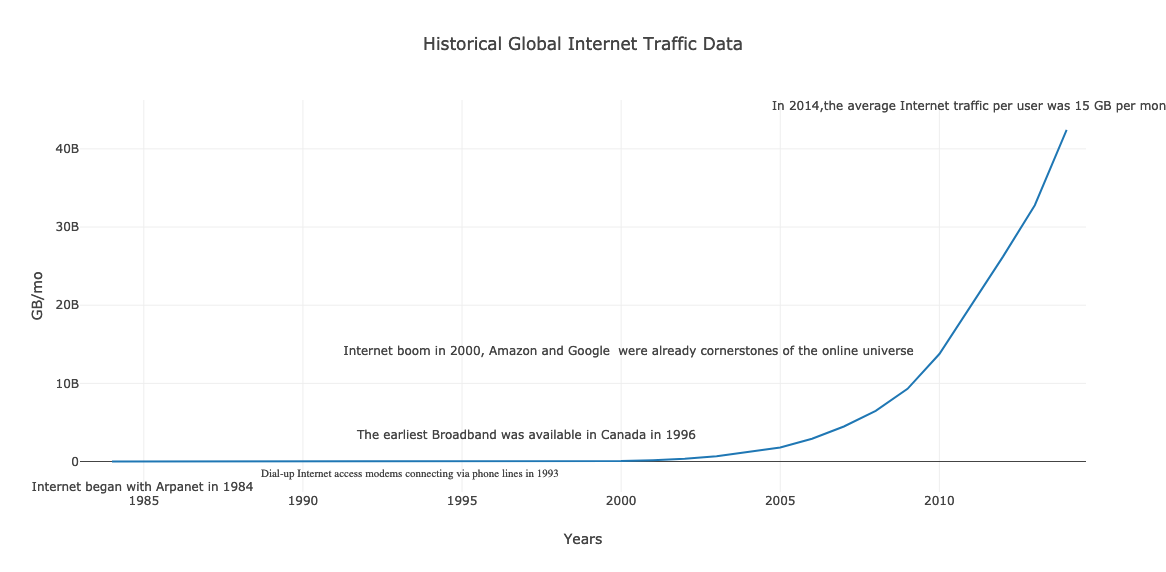
\includegraphics[scale=0.35]{images/Gfk-01.png}
    \caption{Internetverkehr in den letzten Jahrzehnten (02.04.2020)}
    \url{https://plot.ly/~QY/3.embed}
\end{figure}
Der Graph veranschaulicht, wie stark das Datenaufkommen in den letzten Jahrzehnten eine rasante Steilkurve angelegt hat und somit Rückschlüsse darauf ziehen lässt, mit welchen immensen Datenmengen wir es heutzutage zu tun haben. Und das erst bei einer relativ kurzen historischen Periode.
\par
Heute im 2. Jahrzehnt dieses Jahrhunderts ist eine stetig wachsende Wichtigkeit dieses neu begründeten Bereichs der Daten-Analyse eminent. Dadurch ist auch für unseren Auftraggeber, die Firma MIC, ein aufkommendes Interesse in diesen Bereich entstanden. Aus diesem Anlass wurde uns die Aufgabe zu teil, uns mit der Thematik auseinanderzusetzen und Unternehmungen in diesen Bereich mit anzustoßen.
\newpage
\section{Ausgangslage}
Das Thema des ETL-Prozesses und Datenanalyse ist daher für uns von Interesse, da es sich um eine Thematik handelt, welche in unserer HTL-Ausbildung wenig vorkommt. Die Erarbeitung von etwas für uns komplett Neuem steht dabei klar im Fokus. 

Bei ETL handelt es sich keinesfalls um ein neues Konzept. Viele bereits vorhandene ETL-Tools erfordern jedoch eine klare Einlassung auf ein bestimmtes Unternehmen, was für eine Abhängigkeit sorgt. Werden also schnell bestimmte Funktionalitäten gebraucht, welche nicht vom Anbieter angeboten werden, oder welche nicht zu kosteneffizienten Wegen zu erreichen sind, hat man ein Problem. Mithilfe dieser Arbeit sollte eine unabhängige Basis gelegt werden. 

\subsection{Verwandte Arbeiten und Projekte}
Unsere Arbeit ist nicht die Einzige, welche sich mit der Thematik des ETL-Prozesses und deren Analyse auseinandersetzt. Neben unserer Arbeit hat die MIC auch intern an einem Prototypen im Bereich der ETL-Prozesse und Datenanalyse gearbeitet. Im Unterschied zu unserem Projekt sollte dieser aber restriktivere Anforderungen in der Technologiewahl einhalten. 
\vspace{5mm}\par
Darüber hinaus wurde uns als Einführung in die Materie die Masterarbeit „Entwicklung flexibler und erweiterbarer ETL- Systeme für die internationale Zollabwicklung“ aus dem Jahre 2018 von Dominik Schachner, BSc, zur Verfügung gestellt. Auch diese Arbeit wurde im Rahmen einer Kooperation mit der MIC erstellt.
\vspace{5mm}\par
ETL-Lösungen müssen aber nicht umbedingt selbst implementiert werden. Je nach Bedarf und Datenquelle bieten verschiedenste Anbieter, wie IBM, Amazon, Google, eigene Lösungen an.
\par
Der Unterschied und Ansatz unserer Arbeit liegt darin möglichst modular aufgebaut zu sein und so eine einfache Erweiterbarkeit bieten zu können.


\newpage
\section{Struktur der Diplomarbeit}
In der Aufgabenstellung gehen wir darauf ein, was die Erwartungen der beiden kooperierenden Parteien - der Firma MIC und uns - für die Arbeit war.
\vspace{5mm}\par
Darauf folgend legen wir die theoretischen Grundlagen, auf welchen unsere Arbeit beruht, dar.
Dies geschieht in der logischen Reihenfolge des Datenflusses, beginnend von den Datenquellen über die Verarbeitung bis zur Darstellung.
\vspace{5mm}\par
Im Kapitel Werkzeuge legen wir da, welche Mittel wir für diese Arbeit verwendet haben. Im Unterkapitel Arbeitswerkzeuge werden die Werkzeuge beschrieben, welche uns bei der Entwicklung geholfen haben, aber selbst kein Bestandteil des Prototyps an sich sind. Bei Technologien werden jene erläutert, welche Teil des Prototyps sind. So ist Docker Teil der Technologien, da die einzelnen Bestandteile des Prototyps systemunabhängig über geschriebene Dockerfiles erst zum Zusammenschluss kommen. AWS hingegen ist nur die Plattform, welche die Möglichkeit veranschaulichen soll, dass der Prototyp auf einem Cloud-Service lauffähig gemacht werden kann, indem dieser durch Docker eine Systemunabhänigkeit erreicht.
\vspace{5mm}\par
In der “Praktischen Umsetzung” legen wir unseren Schaffensprozess für den Prototypen dar. 
Dieses Kapitel behandelt dafür vier Punkte. Erstens beschreibt es die Konfiguration und Einrichtung der Werkzeuge. Zweitens erläutert es aufkommenden Hürden bei der Realisierung. Drittens beschreibt es den Code in den geschriebenen Modulen. Viertens legt es argumentativ die Entscheidungsprozesse dar.
\vspace{5mm}\par
Zu guter Letzt legen wir im Fazit unsere Meinung und Erfahrungswerte zu dieser Arbeit dar.

\section{Projekt und Dokumentation}
Der Prototyp, seine einzelnen Module, die CI-Tätigkeiten und die Dokumentation sind online in folgendem Repository zu finden:
\href{https://github.com/soyabeantec/AKK}{https://github.com/soyabeantec/AKK}
\chapter{Aufgabenstellung[AA]}
\section{MIC Gedanke}
Die Aufgabenstellung der Firma war es, neue Technologien zu benutzen und anzuwenden. Im Hauptfokus des Unternehmens stand es AWS \ref{ssec:aws} zu benutzten. Die einzige Funktion, die benutzt wurde, war EC2 \ref{ssec:ec2}. Ein weiterer Faktor war eine ältere Masterarbeit aufzugreifen und diese weiter zu bearbeiten. In dieser Masterarbeit ging es darum, Daten aus verschiedensten Quellen zu analysieren und darzustellen. Das finale Ziel der Arbeit war es einen funktionsfähigen Prototypen zu erstellen, der Daten entnimmt, transformiert und diese schlussendlich für Kundinnen und Kunden darstellt.
\section{AKK Gedanke}
Unsere Aufgabenstellung war es einen ETL Prozess zu entwickeln und mit einem Data Warehouse zu verbinden. Durch das Data Warehouse werden die aufbereitenden Daten weiter an die Visualisierungssoftware geschickt und angezeigt. Auch war ein Teil der Arbeit neue Technologien kennenzulernen und anzuwenden (z.B.: AWS \ref{ssec:aws} oder das Datawarehousing \ref{ssec:dw}).
\chapter{Theoretische Grundlagen}
\section{Architektur[FK]}
Anmerkung: Folgendes wurde auf Basis von diesen Quellen geschrieben: (vgl. \cite{bashar_architekturvorgabe_2019})
Die Architektur wie das System am Ende ausschauen soll wurde uns Vollständig von unserem Auftraggeber der MIC vorgegeben. Wir durften auch nur eingeschränkt entscheiden welche Technologie wir dafür verwenden. 
Die Anforderungen der Architektur sind jene, dass das System nach ICES - Independent, Configurable, Extensible und Scalable aufgebaut ist. Dieses Konzept wurde aus dem Grund gewählt um dem System ein möglichst großes Anwendungsgebiet zu ermöglichen. Da jede Firma einen anderen Systemhintergrund hat und nur so eine Näherung an „one-size-fits-all“ möglich ist. 
Folgende Grafik ist die Grundlage für die Gesamte folgende Arbeit.
\begin{figure}[H]
    \centering
    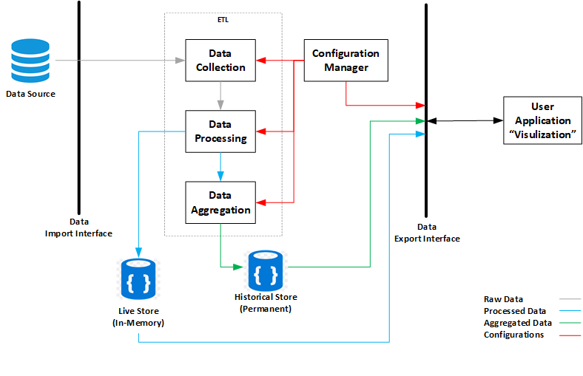
\includegraphics[scale=0.9]{images/architektur_uebersicht.png}
    \caption{Systemarchitektur Uebersicht}
    \label{img:architektur_uebersicht}
\end{figure}
Am Anfang (Links) bei der „Data Source“ (Datenquelle) werden alle Daten aus der MIC Datenbank genommen. Im Kapitel Extract [\ref{sec:extract}] wird noch genauer darauf eingegangen wie der Prozess Abläuft. 
Sobald die Daten extrahiert sind werden sie verarbeitet, Aggregiert (Kapitel Transform [\ref{sec:transform}])  und entweder in die Redis In-Memory Datenbank oder in den Permanenten Speicher der Cassandra Datenbank gespeichert (Kapitel Load [\ref{sec:load}]). 
Schlussendlich kommen die Daten aus den Datenbanken über eine REST [\ref{sec:REST}] Schnittstelle in den Visualisierungsprozess (Kapitel Visualization [\ref{sec:visualization}]). Dort kommen sie in eine Elasticsearch [\ref{sec:ES}] Datenbank, um dem Visualisierungstool Kibana [\ref{ssec:Kibana}] optimalen Zugriff zu verschaffen.
Der „Configuration Manager“ ist in unserer Diplomarbeit leider weggefallen, weil unsere Arbeit nur einen Prototypen darstellen soll und wir uns deswegen auf die wichtigsten Dinge Konzentriert haben.
Folgend werden die Schritte einzeln Erklärt wie sie geplant waren.
\subsection{Import-Interface}
Dieses Modul soll eine Verbindung zu Datenquellen und API's [\ref{sec:API} herstellen um auf der Datenquelle Abfragen ausführen zu können. Datenquellenspezifische Dinge wie, … (hide, network, security and query issues from the system)… sollen abstrahiert werden.
\begin{figure}[H]
    \centering
    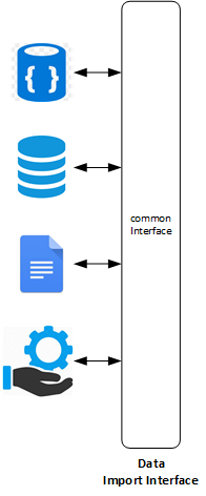
\includegraphics[scale=1]{images/arch_dataImportInterface.png}
    \caption{Systemarchitektur Import-Interface}
    \label{img:arch_dataImportInterface}
\end{figure}
Beim Import soll durch ein Interface eine zusätzliche Schicht auferlegt werden um Daten
in den verschiedensten Formaten entgegennehmen zu können. Dieser modulare Ansatz
ermöglicht es auch durch ein simples Tauschen der Module an eine anderen
Systemschnittstellen sich einzuwählen. 
\subsection{Data-Collection}
Dieses Modul soll periodisch Daten von der Datenquellen ziehen. Abhängig von dem Datenformat müssen wir ggf. die Daten parsen um diese weiterzuverarbeiten. Mit den gelieferten Daten bilden wir dann ein Unified-Object, diesem fügen wir einen Zeitstempel und eine Stream-ID (zur späteren Identifikation) hinzu.
\begin{figure}[H]
    \centering
    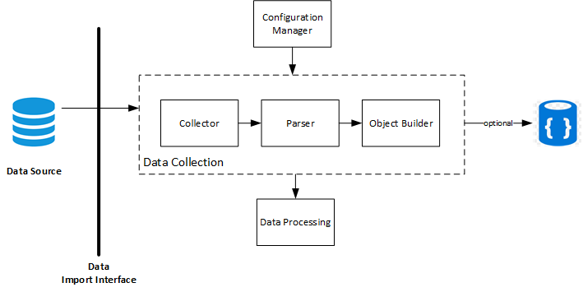
\includegraphics[scale=1]{images/archDataCollection.png}
    \caption{Systemarchitektur Data-Collection}
    \label{img:archDataCollection}
\end{figure}
\subsection{Data-Processing}
Wie folgende Grafik zeigt bekommt das Modul rohe Datenströme aus dem Data-Collection Modul.

Im Modul können verschiedenste Verarbeitungsmethoden angewendet werden. Um zum Beispiel bestimmte Daten herauszufiltern welche nicht benötigt werden. Eine andere Möglichkeit wäre aber auch Datensätze die Gemeinsamkeiten Aufweisen auf einen Gemeinsamen Datensatz zusammenzuführen. Nachdem wir Dokumentenorientierte Datenbanken verwenden ist die Schemafreiheit an dieser Stelle besonders Wichtig. 

Sobald die Prozesse fertig sind kommen die bearbeiteten Datenströme in das nächste Modul die Daten Aggregation. Optional werden die Daten auch in einer In-Memory Datenbank zwischengespeichert.
\begin{figure}[H]
    \centering
    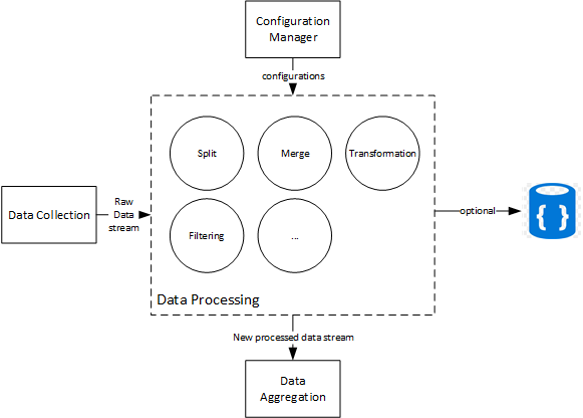
\includegraphics[scale=1]{images/archDataProcessing.png}
    \caption{Systemarchitektur Data-Processing}
    \label{img:archDataProcessing}
\end{figure}
\subsection{Data-Aggregation}
Die verarbeiteten Daten kommen in das Aggregations Modul. Das Aggregations Modul besitzt zwei verschiedene Konfigurationen nämlich den Aggregationsplan und die Aggregationsfunktion. In der Folgenden Grafik wird Dargestellt wie diese Aggregationen aussehen können. Außerdem können mehrere Aggregationspläne für dieselben Daten definiert werden. 

Sobald die Daten Aggregiert wurden kommen sie in den Permanenten Speicher
\begin{figure}[H]
    \centering
    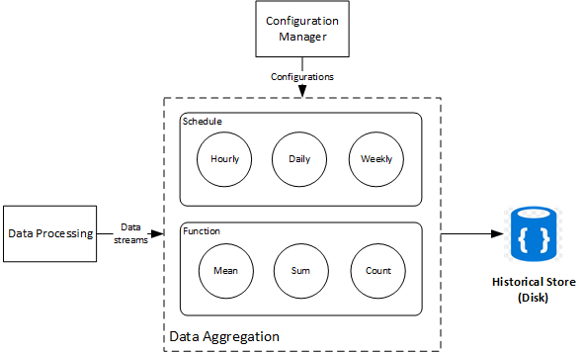
\includegraphics[scale=1]{images/archDataAggregation.png}
    \caption{Systemarchitektur Data-Aggregation}
    \label{img:archDataAggregation}
\end{figure}
\subsection{Data-Interface}
Das Dateninterface ist die Zentrale Schnittstelle um die zuvor verarbeiteten Daten in die Visualisierungsapplikation zu bekommen.
Dieses Interface wird als REST [\ref{sec:REST} Schnittstelle realisiert. Somit kann auf den Permanenten Speicher sowie als auch auf die Live Daten Abfragen gemacht werden. Die Visualisierungsapplikation kann auch eine Metabeschreibung der Daten (Namen, Typen usw.) abrufen.
\begin{figure}[H]
    \centering
    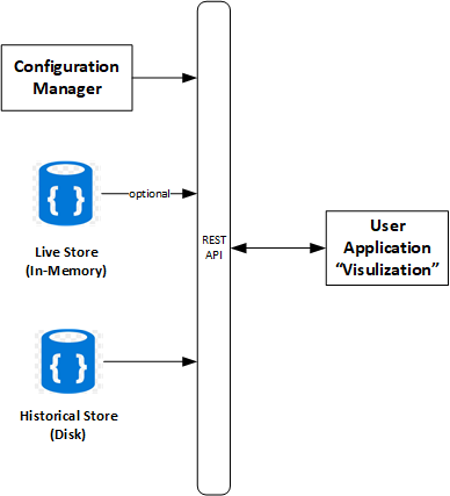
\includegraphics[scale=1]{images/archDataInterface.png}
    \caption{Systemarchitektur Data-Interface}
    \label{img:archDataInterface}
\end{figure}
\newpage
\section{Datenquellen[EK]}
Ein ETL-Prozess sollte die Möglichkeit bieten, aus vielen verschiedenen Quellen Daten zu extrahieren. Im Kontext der MIC handelt es sich bei diesen um Daten des Zollwesen. 
Dadurch, dass die Möglichkeit eines Zugriffs auf ein Echtzeitsystem nicht gegeben war, sollte eine vereinfachte, abgeflachte Datei diese Zolldeklarationen für die Extraktion beinhalten. Diese Datei wiederum wird durch einen Generator im JSON-Format bereitgestellt.
\vspace{5mm}\par
Wie ist nun eine solche abgeflachte Zolldeklaration aufgebaut?
\vspace{5mm}\par
Jede Zolldeklaration, welche generiert wird, ist genau gesehen eine Rechnungszeile. Eine solche Zeile beinhaltet die Wareninformationen, wie ihre Id, die Kosten, die abzugebenden Steuern, die Anzahl, ihr Präferenzcode etc. Zu jeder Rechnungszeile, liegen die übergeordneten Informationen da. Dies bedeutet, wir wissen zu welcher Deklaration und Lieferung diese Zeile gehört. 
Diese gibt Aufschlüsse über das zuständige Zollamt und durch welches es ins Land kam, das Datum, das Ursprungsland, ob die Fracht über Container transportiert wird oder nicht und mit welchem Transportmittel diese zur Grenze kam und mit welchen Transportmittel diese im Inland weitertransportiert wird. Zusätzlich liegen zu allen drei Parteien - Exporteur, Importeur und Lieferant - die Adressdaten und ihre Registrierungsnummer zu eindeutigen Identifizierung zur Verfügung. Dies sind noch nicht alle Informationen, welche vorhanden sind, jedoch sind diese die wichtigsten.

\newpage
\section{ETL-Definition[EK]}
„ETL (oder Extrahieren, Transformieren, Laden) ist ein Prozess der Datenintegration, welcher drei Schritte umfasst: Extraktion, Transformation und Laden. Kurz gesagt, entnimmt ETL Rohdaten aus mehreren Quellen, konvertiert sie für die Analyse und lädt diese Daten in ihr Warehouse“ \cite{ETL-Explained}
\begin{figure}[H]
    \centering
    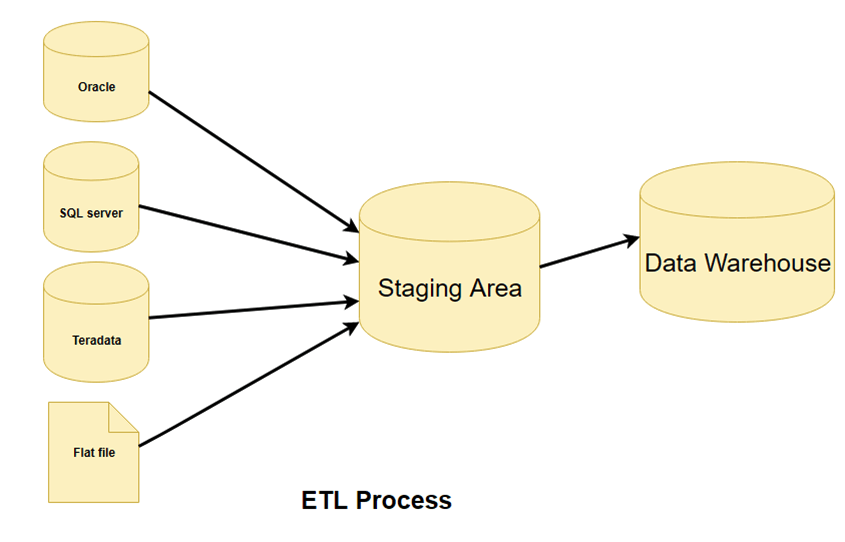
\includegraphics[scale=0.5]{images/etl-staging-area.png}
    \caption{ETL-Staging-Area (02.04.2020)}
    \url{https://www.guru99.com/images/1/022218_0848_ETLExtractT1.png}
\end{figure}
Wie aus der Grafik zu entnehmen ist, kann man den ETL-Prozess neben der Unterteilung in Extraktion, Transformation und Laden auch in diese drei Sektionen unterteilen: Datenquellen, Staging-Area und das Data-Warehouse.


\newpage
\section{Extract[EK]}\label{sec:extract}
Ein jeder ETL-Prozess beginnt mit der Extraktion der zu verarbeitenden Daten. Diese Daten können aus verschiedensten Quellen kommen und eine große Variation in ihrer Strukturierung aufweisen. Somit sollten diese Daten zuerst aufbereitet werden, da ein direkter Transfer ins Data-Warehouse für fehlerhafte und damit unverwendbare Daten sorgen könnte. Verschiedenste Gründe können dafür vorliegen. Es können die Daten von der Quelle selbst bereits beschädigt sein, oder durch ihre Vielzahl an Datenformaten zu einer Unvereinbarkeit dieser kommen.
\vspace{5mm}\par
Um hier Abhilfe zu schaffen, kommen die Daten zuerst in eine sogenannte Staging-Area. Diese wird dafür verwendet, um die Daten so aufzubereiten, dass in ihnen nur noch die Informationen enthalten sind, welche vom Data-Warehouse benötigt werden und in solch einer Form, dass diese vereinheitlicht organisiert sind. Darüber hinaus entsteht ein Möglichkeitsfenster, um diese Daten auch zu validieren, was je nach Datenquelle mehr oder weniger von Nöten ist. Folgend ein paar Beispiele, welche aufzeigen sollen, welche Möglichkeiten der Validierung während der Extraktion vorliegen:
\begin{itemize}
  \item Abgleichen von Datensätzen mit der Quelle
  \item Überprüfung der Richtigkeit der Datentypen
  \item Entfernen von Duplikaten
  \item Entfernen von fragmentierten Daten
\end{itemize}
Ein wichtiger Punkt des Extrakts ist, dass die Abfrage der Daten aus der Quelle für keine Performanceeinbußen sorgen sollte. Die Begründung dafür ergibt sich aus einer Tatsache. Meist kommen die Daten, welche für einen ETL-Prozess von Interesse sind von einem Live-Production-System beziehungsweise einer Datenbank. Das bedeutet, dass es sich bei diesen um systemkritische Elemente handelt, ein Performanceeinbruch könnte schwerwiegende Probleme in der Haupttätigkeit des Systems hervorrufen und bei Unternehmen gar zu Einkommenseinbußen führen. Die Eigenschaften einer guten Extraktion bestehen also darin, dass wir Fehlerquellen vorzeitig abfangen können und dass Daten so direkt wie möglich aus der Quelle entnommen werden - Transformationen sollen, wenn von Nöten erst in der Staging-Area im ETL stattfinden und nicht bei der Abfrage.
(vgl. \cite{ETL-Process} \& \cite{ETL-Explained})
\newpage
\section{Transform[EK]}\label{sec:transform}
Nachdem alle Datenquellen im Extrakt ihre speziell zugeschnitten Extraktionslösungen erhalten haben, welche die Besonderheiten der Datenquellen berücksichtigen, kann nun die Phase der Transformation eingeleitet werden. In diesem Teil kommen die validierten aber noch nicht nutzbaren Rohdaten an. Dieser Schritt ist auch jener, welcher dem ETL-Prozess eine große Wertschöpfungsmöglichkeit erlaubt, indem die Daten so aufbereitet werden, dass möglichst aussagekräftige BI-Reports daraus erstellt werden können. Damit diese Aufbereitung erfolgreich ablaufen kann, werden die multiplen Rohdatensätze normalisiert und in ein einziges Systemformat gebracht. 
\vspace{5mm}\par
Nicht alle extrahierten Daten benötigen zwingend eine Transformation, solche Daten werden Pass-Through-Daten genannt.
\vspace{5mm}\par
Eine gewisse Komplexität kommt durch Probleme der Datenintegrität auf. So kann es vorkommen, dass bestimmte Daten zusammen gehören, aber einen andere Identifikation tragen. Die Stadt „Vienna“ und „Wien“ bezeichnen den selben Ort, aber in verschiedenen Schreibweisen. Anders kann dies auch vorkommen: Daten tragen eine gleiche Identifikation und gehören so eigentlich nicht zusammen. Zum Beispiel gibt es Städte in der Welt, welche den gleichen Namen tragen, aber auf zwei verschiedenen Kontinenten liegen: Paris in Frankreich ist nicht Paris in Texas. Visuell wird dies nochmals durch die folgende Grafik veranschaulicht:

(vgl. \cite{ETL-Process} \& \cite{ETL-Explained})
\begin{figure}[H]
    \centering
    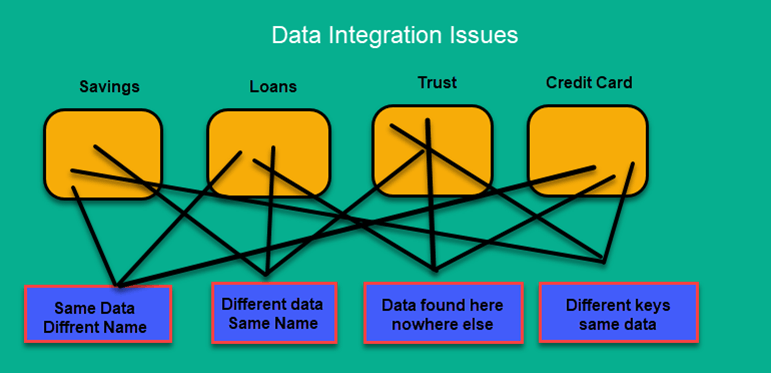
\includegraphics[scale=0.5]{images/etl-integration-issues.png}
    \caption{Probleme der Datenintegration (02.04.2020)}
    \url{https://www.guru99.com/images/1/022218_0848_ETLExtractT2.png}
\end{figure}
\newpage
Es gibt ein Vielzahl von Validationen, welche im Laufe eines Transform-Prozesses auftreten können. Ein paar Beispiele:
\begin{itemize}
    \item Filtern von Daten - nur spezielle Daten sollten an den Load-Prozess übergeben werden
    \item Benötigte Felder sollten keine leeren NULL-Felder enthalten
    \item Maßeinheiten sollten alle in ein bestimmtes Format umgewandelt werden
    \item Die Datensätze sollten nach einem speziellen Kriterium sortiert werden
\end{itemize}
Allgemein lässt sich sagen, dass in die Validation alle Tätigkeiten fallen können, welche die Daten aufbereiten und so besser nutzbar machen. Der Fokus liegt hier, im Unterschied zur eigentlichen Datenanalyse, in der Tatsache, dass noch keine Schlüsse aus diesen Daten gezogen werden sollen, sondern nur dies im späteren Verlauf erleichtert.
\vspace{5mm}\par
Zusammenfassend kann gesagt werden, dass es sich bei der Transformation um einen sehr angepassten Prozess handelt. Somit ist eine große Variation in der Komplexität, je nach Anforderung und Datensets, möglich.
(vgl. \cite{ETL-Process} \& \cite{ETL-Explained})
\newpage
\section{Load[AA]}\label{sec:load}
Folgende Informationen wurden aus nachstehender Quelle bezogen. (vgl. \cite{guru_etl_2020}) \\

In diesem Schritt werden die Daten in einem Datenspeicher gelagert. Dies kann entweder ein normales File beziehungsweise ein Data Warehouse sein. Da viele Daten in einer kurzen Zeit, also über eine Nacht, in das Data Warehouse geladen werden sollen, muss dieser Schritt für Performanz optimiert werden.

Ein anderer wichtiger Punkt ist es, Daten ohne den Verlust von Datenintegrität wiederherstellen zu können. Der/Die Data Warehouse AdministratorIn muss diesen Schritt überwachen, weiterführen und stoppen während die Server Performanz weiter bestehen soll.
\subsection{Typen des Ladens}
\begin{itemize}
\item Initial Load \mbox{} \\
In diesem Load werden alle Tabellen im Data Warehouse bespielt.
\item Incremental Load \mbox{} \\
Hier werden alle Änderungen die passiert sind getätigt und wenn es nötig ist auch in einem periodischen Abstand durchgeführt.
\item Full Refresh \mbox{} \\
Bei einem Full Refresh werden alle Daten aus einer oder mehrerer Tabellen gelöscht und mit frischen Daten befüllt.
\end{itemize}
\subsection{Verifikationen des Ladens}
\begin{itemize}
\item Das Key Feld der Daten darf nicht fehlen oder Null sein.
\item Modellierungsansichten müssen auf Basis der Tabellen getestet werden.
\item Die BI Reports überprüfen Fakten- und Dimensionstabellen.
\item Überprüfen der Daten in den Dimensionstabellen.
\end{itemize}
\newpage
\section{Data Warehouse[AA]}\label{ssec:dw}
Referenzinformationen für dieses Unterkapitel stammen aus dieser Quelle. (vgl. \cite{ionis_dwh_2020})
\subsection{Definition}
Ein Data Warehouse (DW) ist ein zentrales Datenbanksystem, um Daten effektiv in einem Unternehmen analysieren zu können. Zahlreiche Unternehmen laden ihre historischen Daten in ein Data Warehouse, um jene Daten zu analysieren. Um mit ihnen Prognosen geben zu können, wie das Unternehmen in der Zukunft agieren soll. Im Data Warehousing gibt es zwei Daten, die unterschieden werden müssen(\ref{ssec:Operative-Daten} \& \ref{ssec:Dispositive-Daten}). Außerdem ermöglicht ein Data Warehouse die Aggregation betrieblicher Kennzahlen im Rahmen des OLAP (Online Analytic Processsings).\\
Durch das Sammeln aller relevanten Unternehmensdaten dient das Data Warehouse auch als Wissens Managementsystem. Im Regelfall werden den Anwendern nur der Lesezugriff gewährt, aber keine Schreibrechte, um Daten zu ändern oder gar zu löschen. Ein Data Warehouse ist zudem auch noch Datenbasis für Data Mining Methoden und ist die Grundlage aller Überlegungen im Rahmen des Leistungsmanagements und der strategischen Unternehmensausrichtung.
\subsection{Operative Daten}\label{ssec:Operative-Daten}
Bei diesen Daten handelt es sich um transaktionsorientierte Daten und Informationen, die während des Tagesbetriebs in einem Unternehmen anfallen und von Administrations- und Abrechnungssystemen generiert werden. Zu Datenquellen dieser Daten gehören Buchhaltungsprogramme, Warenwirtschaftssysteme, Enterprise-Ressource-Planung (ERP) oder Auskunft- und Bestellsysteme.
\subsection{Dispositive Daten}\label{ssec:Dispositive-Daten}
Werden operative Daten in ein zentrales System aggregiert, gelagert und für Analysen benutzt und verarbeitet, spricht man von dispositiven Daten.
\newpage
\subsection{Data-Warehouse-Architektur}
Das Beschaffen und die Auswertung der Daten eines Data Warehouses wird Data Warehousing genannt und umfasst drei Phasen.
\begin{itemize}
\item Datenbeschaffung und Datenintegration
\item Datenhaltung
\item Datenauswertung und Datenanalyse
\end{itemize}
Diese Phasen spiegeln sich in der Referenzarchitektur von Data Warehouse Systemen wider. Natürlich unterscheidet sich die Systemarchitektur eines Data Warehouses je nach Produkt und Anbieter, jedoch orientiert sich der technische Aufbau an einem Muster, das sich erneut in drei Ebenen gliedern lässt.
\begin{itemize}
\item Datenerfassungsebene
\item Datenhaltungsebene
\item Datenbereitstellungsebene
\end{itemize}
Es gibt auch eine zentrale Kontrollkomponente. Dies ist der Data Warehouse Manager, der jeder Ebene spezielle Administrationsfunktionen zuordnet. Die einzelnen Komponenten eines Data Warehouses müssen nicht von einem einzigen Anbieter stammen, denn jeweilige Services können von unterschiedlichen Softwareprodukten oder Individuallösungen bereitgestellt werden.
In dieser Graphik wird das gesamte Referenzmodell eines Data Warehouses bildlich dargestellt.
\begin{figure}[H]
\centering
  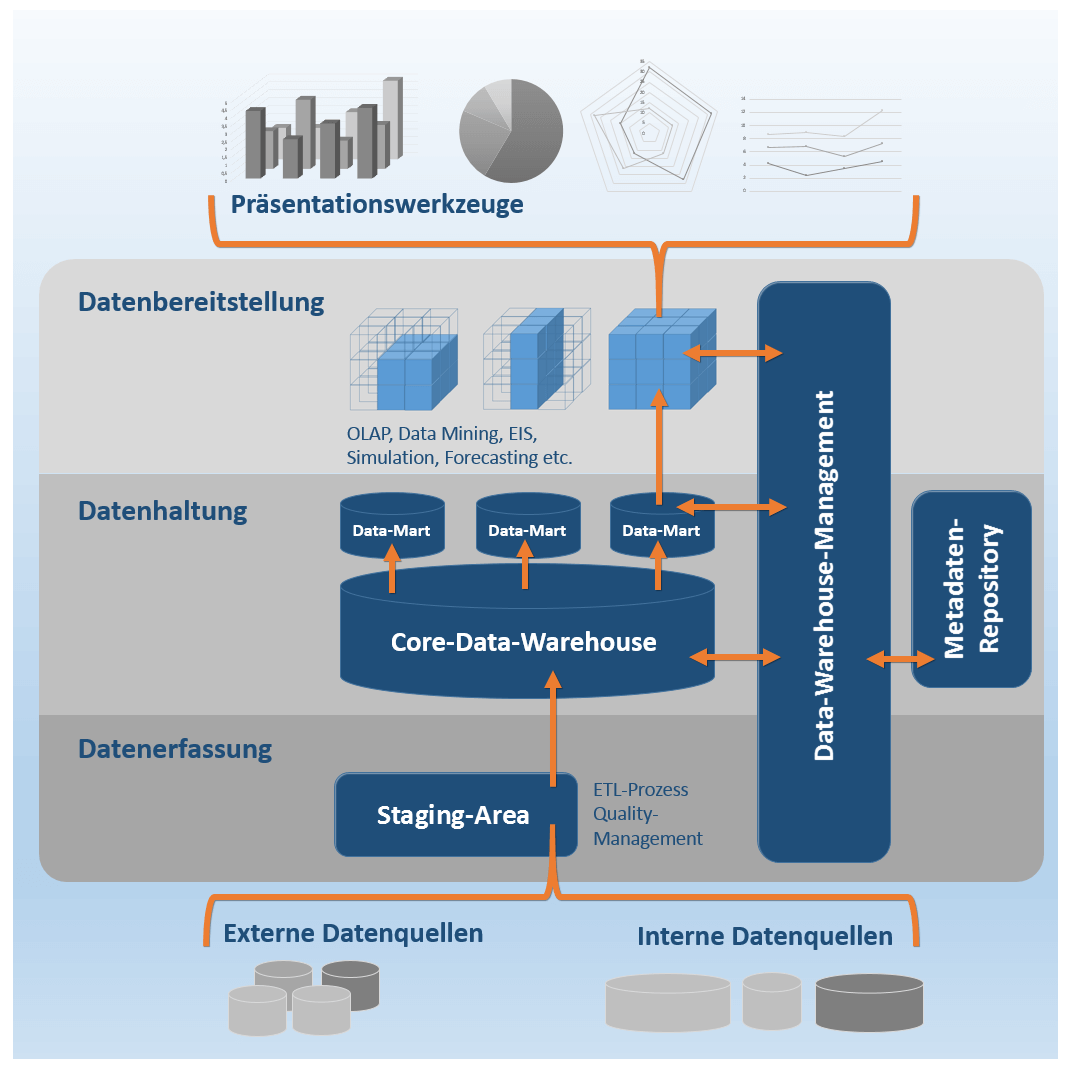
\includegraphics[scale=0.4]{images/data-warehouse-referenzarchitektur.png}
  \caption[DWH Referenzarchitektur (01.04.2020)]{DWH Referenzarchitektur (01.04.2020)}
  \url{https://www.ionos.at/digitalguide/fileadmin/DigitalGuide/Screenshots/data-warehouse-referenzarchitektur.png}
  \label{fig:DWH-RA}
\end{figure}
\newpage
\subsection{Datenerfassungsebene}
Bevor das Data Warehouse Daten bekommen kann, müssen diese oft sehr heterogenen Daten in eine einheitliche Form transformiert werden. Ein Data Warehouse bekommt Daten sowohl aus internen (\ref{ssec:Interne-Daten}) als auch aus externen (\ref{ssec:Externe-Daten}) Datenquellen. Systeme in dieser Ebene stellen Schnittstellen zu operativen Systemen eines Unternehmens bereit und kommen in der ersten Phase des Data Warehousings zum Einsatz. Zentrale Funktionen dieser Phase sind die Datenbeschaffung und Datenintegration. Diese Ebene eines Data Warehouses kann auch eine Staging Area(\ref{ssec:Staging-Area}) beinhalten. Da unterschiedlichste Daten von verschiedensten Quellen in ein DW zusammengefügt werden, muss sich die Datenintegration auf diverse Werkzeuge verlassen, die eine Transformation und Bereinigung der Daten ermöglichen. Diese Werkzeuge können in folgende Kategorien, unterteilt werden (\ref{ssec:Data-Migration} \& \ref{ssec:Data-Scrubbing} \& \ref{ssec:Data-Auditing}). Nach der Datenintegration folgt die Übernahme der Daten in die zentrale Datenbank, in das Core Data Warehouse. Dieser Schritt wird durch Programme unterstützt, die folgende Funktionen bereitstellen.
\begin{itemize}
\item Integritätsbedingungen prüfen
\item Daten sortieren
\item Aggregationen berechnen
\item Zugriffsstrukturen berechnen
\item Daten für einen effizienten Zugriff partitionieren
\end{itemize}
\subsection{Interne Daten}\label{ssec:Interne-Daten}
Interne Daten können von operativen Systemen kommen. Da wären zuallererst, Enterprise Resource Planning-Systeme (ERP) und Customer Relationship Management Systeme(CRM). Auf der anderen Seite können Daten aus operativen Datenbanken bezogen werden. Aus Content Management Systemen(CMS) oder auch aus Flat Files. Beispiele zu diesen wären Excel-, CSV- und Textdateien. Mails und andere Quellen können auch Daten enthalten, die wichtig für ein Data Warehouse sind.
\subsection{Externe Daten}\label{ssec:Externe-Daten}
Dies sind Daten die von externen Dienstleistern stammen. Aus externen Anwendungen und Systemen, wie etwa Websites, Social Media und Cloud Services.
\subsection{Staging Area eines DW}\label{ssec:Staging-Area}
Eine Staging Area ist ein temporärer Bereich der Datenbank, in dem die Vorverarbeitung der zu ladenden Daten stattfindet. Bei mehr komplexen ETL-Prozessen ist so ein Staging erforderlich.
\subsection{ETL für Datawarehouse}\label{ssec:ETL-DW}
Die meisten Data Warehouse stellen im Rahmen der Datenintegration, OLAP-Funktionalitäten zur Verfügung. Diese Funktionalitäten ermöglichen es, Daten in mehrdimensionalen Strukturen darzustellen. Durch den vorher beschriebenen ETL Prozess(\ref{ssec:ETL-DW}) werden Daten aus verschiedensten Quellen extrahiert, danach vorbereitet und anschließend transformiert. Daraufhin werden diese transformierten Daten in das Data Warehouse geladen und dort abgespeichert. Da OLAP eine Analysemethode ist, die der Verdichtung managementrelevanter Unternehmensdaten dient, ist es möglich dieses Verfahren auf den ETL-Prozess zu übertragen.
\subsection{Data Migration Tools}\label{ssec:Data-Migration}
Programme für Datenmigrationen sind dazu da, einfache Transformationsregeln zu definieren und heterogene Ausgangsdaten in ein einheitliches Zielformat zu transformieren.
\subsection{Data Scrubbing Tools}\label{ssec:Data-Scrubbing}
Programme die Data Scrubbing unterstützen, stützen sich auf den Fuzzy Logic Ansatz sowie neuronale Netze. Ziel dieses Ansatzes ist es, die Datenqualität zu verbessern. Dies geschieht indem Fehler, Lücken und Wiederholungen in Datensätzen durch vordefinierten Regeln, Algorithmen oder Lookup Tabels ausgebessert werden. In diesem Fall könnte man auch von Qualitätsmanagement sprechen.
\subsection{Data Auditing Tools}\label{ssec:Data-Auditing}
Dieses Werkzeug kommt zum Einsatz um Regeln und Beziehungen zwischen Daten zu ermitteln. Auch ist es so möglich, Daten zu identifizieren, die gegen die Regeln verstoßen und somit fehlerhaft sind.
\newpage
\subsection{Datenhaltungsebene}
Dies ist die Kernebene des Data Warehouses. In dieser Ebene liegt das Core Data Warehouse. Daten, die extrahiert worden sind, werden in das Data Warehouse meist in mehrdimensionalen Matrizen gespeichert. Doch wird für die Speicherung bestimmte Schemata verwendet. Dies sind das Star-(\ref{ssec:Star-Schema}) oder das Snowflake Schemata(\ref{ssec:Snowflake-Schema}). Diese beinhalten jedoch selten den gesamten Datenbestand des Data Warehouses. Um effiziente Auswertung aus den Daten zu erstellen, werden üblicherweise Datenausschnitte, sogenannte Data Marts(\ref{ssec:Data-Marts}) angelegt.
\subsection{Data Marts}\label{ssec:Data-Marts}
Ein Data Mart ist eine Kopie eines Bestandteils des Data Warehouses. In der Regel sind diese Daten nicht persistent und Data Marts werden oft nur als Zwischenspeicher genutzt. Es gibt jedoch auch unabhängige Data Marts die separate Datenausschnitte dauerhaft lagern und speichern können.
\subsection{Faktentabelle}\label{ssec:Fakten-Tabelle}
Die Faktentabelle beinhaltet verschiedenste Fakten. Diese sind Kennzahlen oder Ergebniszahlen eines Unternehmes, die kontinuierlich in diese Tabelle gespeichert werden.
\subsection{Dimensionstabelle}\label{ssec:Dimensions-Tabelle}
In diesen Tabellen werden Attribute gespeichert, die die Daten der Faktentabelle beschreiben. In einer Dimensionstabelle ist eine Sammlung von Referenzinformationen zu den in der Faktentabelle gespeicherten Ereignissen.
\subsection{3NF}\label{ssec:Dritte-NF}
Alle Data Warehouses können in der dritten Normalform gehalten werden. Doch ist es besser auf andere Schemata auszuweichen, da hier viele Joins getätigt werden müssen um die Daten zu analysieren. Doch hier wird kosteneffizient gespeichert und es kommen keine Redundanzen auf.
\begin{figure}[H]
\centering
  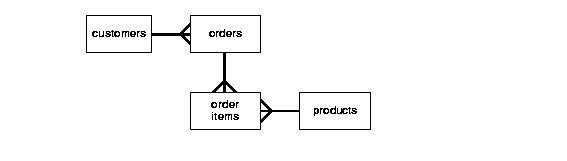
\includegraphics[scale=0.5]{images/3NF.png}
  \caption[3NF (01.04.2020)]{3NF (01.04.2020)}
  \url{https://docs.oracle.com/cd/B10500_01/server.920/a96520/dwhsg108.gif}
  \label{fig:3NF}
\end{figure}
Dieser Auszug wurde durch folgende Quelle inspiriert. \cite{oracle_schema_2020}
\subsection{Star Schema}\label{ssec:Star-Schema}
Bei dem Star Schema handelt es sich um eine Form des Entity Relationship Diagrams oder kurz ERD. Dies ist eine grafische Darstellung der Tabellenstruktur einer Datenbank, bei der die Entitäten sowie die Beziehungen dargestellt werden. Dieses Schema dient der Visualisierung multidimensionaler Datenstrukturen. Jedes Schema besteht aus einer Faktentabelle und mehreren Dimensionstabellen, die sternförmig gruppiert sind. In einem Star Schema ist nur die Faktentabelle mit allen Dimensionstabellen via Fremdschlüssel verbunden. Verbindungen zwischen einzelnen Dimensionstabellen gibt es in diesem Schema nicht.
\begin{figure}[H]
\centering
  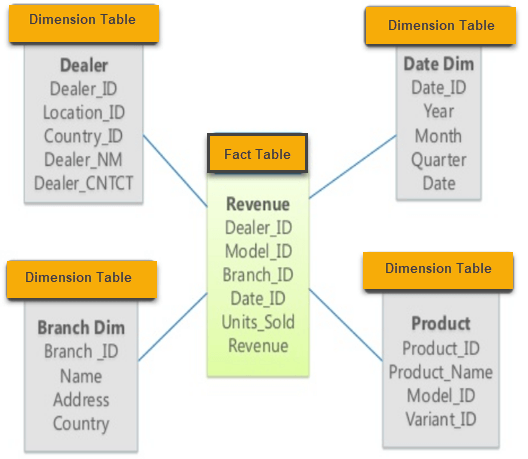
\includegraphics[scale=0.4]{images/Star.png}
  \caption[Star Schema (01.04.2020)]{Star Schema (01.04.2020)}
  \url{https://www.guru99.com/images/1/022218_0758_StarandSnow1.png}
  \label{fig:Star-Schema}
\end{figure}
\newpage
\subsection{Snowflake Schema}\label{ssec:Snowflake-Schema}
Dieses Schema stützt sich im Allgemeinen darauf, dass die Dimensionstabellen normalisiert werden, beziehungsweise Daten nicht mehr redundant in den Dimensionstabellen gespeichert werden. Durch diese Aufteilung der Daten entsteht eine Klassifizierung damit diese hierarchisch gelagert werden. Jene Verzweigung erinnert an eine Schneeflocke. Im Gegensatz zum Star Schema verbraucht das Snowflake Schema viel weniger Speicherplatz. Dies gelingt durch die Aufteilung der Daten auf mehrere Tabellen um so Redundanzen zu vermeiden. Oft werden die Dimensionstabllen noch weiter normalisiert, um bessere Strukturen erreichen zu können. Auf diese Art und Weise wird der Umgang mit Daten erleichtert, da diese, wenn es benötigt wird, nur an einer Stelle angepasst werden müssen. \\
Ein Nachteil ist, dass dadurch nicht nur die Datenstruktur um einiges komplexer wird. Außerdem müssen Tabellen gejoint werden, wenn die Daten benötigt werden. Der Join ist einer der aufwendigsten Datenbankzugriffe die es gibt. In der Praxis wird für die Datenstruktur des Core Data Warehouse oft das Snowflake Schema angewendet, während für einzelne Data Marts das Star Schema benutzt wird.
\begin{figure}[H]
\centering
  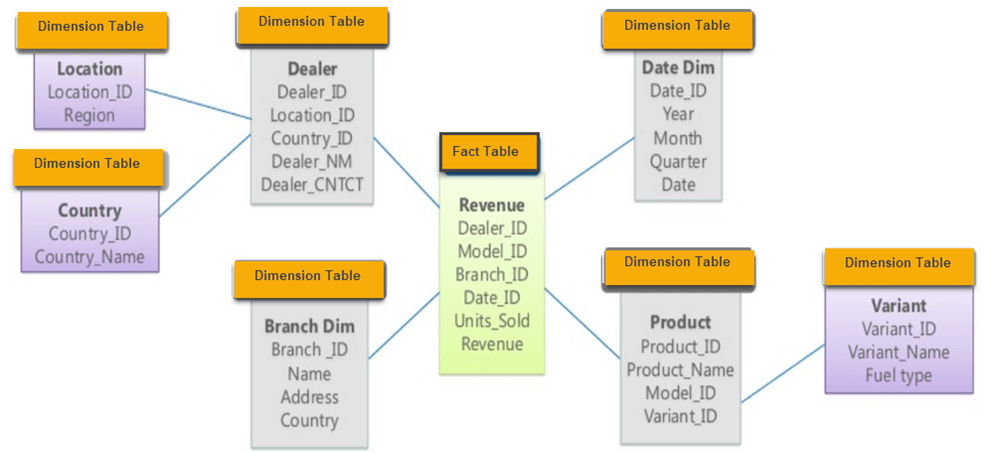
\includegraphics[scale=0.4]{images/Snow.png}
  \caption[Snowflake Schema (01.04.2020)]{Snowflake Schema (01.04.2020)}
  \label{fig:Snowflake-Schema}
  \url{https://www.guru99.com/images/1/022218_0758_StarandSnow2.png}
\end{figure}
\newpage
\subsection{Galaxy Schema}\label{ssec:Galaxy-Schema}
Dieses Schema ist wie das Star- oder das Snowflake Schema ein Datenmodell, das in OLAP Systemen benutzt wird. Der einzige Unterschied zum Snowflake Schema ist, dass es in diesem Schema mehrere Faktentabellen gibt, die mit den gleichen Dimensionstabellen verknüpft sind. Durch dieses Schema können komplexere Unternehmenssituationen und die dabei entstehenden Kennzahlen implementiert und analysiert werden.
\begin{figure}[H]
\centering
  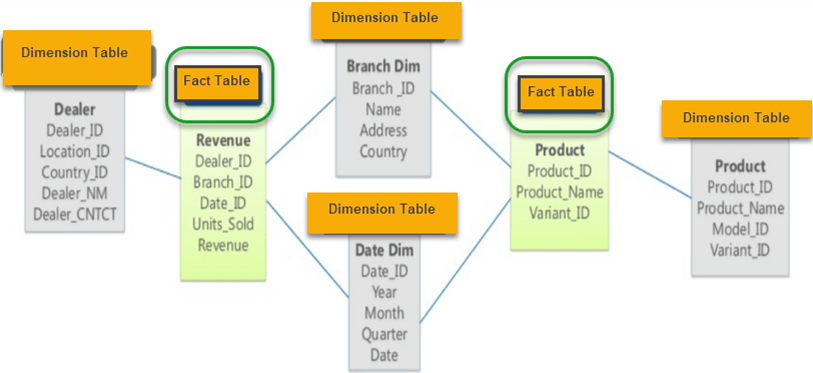
\includegraphics[scale=0.5]{images/Galaxy.png}
  \caption[Galaxy Schema (01.04.2020)]{Galaxy Schema (01.04.2020)}
  \label{fig:Galaxy-Schema}
  \url{https://www.guru99.com/images/1/022218_0758_StarandSnow3.png}
\end{figure}
\newpage
\subsection{OLAP Würfel}\label{ssec:Olap-Cube}
Im Star- beziehungsweise Snowflake Schema wird oft von Dimensionstabellen gesprochen, da sich jede Tabelle als eine Dimension eines OLAP Würfels darstellen lässt. Dies ermöglicht Analysten, die im Data Warehouse gespeicherten Fakten in Relation zu verschieden vielen Referenzinformationen zu setzen, um Kennzahlen wie den Umsatz anhand verschiedener Aspekte mehrdimensional zu analysieren und in diversen Detaillierungsstufen zu untersuchen.\\ 
Die nächste eingefügte Graphik \ref{fig:OLAP-Cube} zeigt die Darstellung eines dreidimensionalen OLAP Würfels, dessen Kanten verschiedene Dimensionen anzeigen. Die Länge wird durch die Anzahl der Zellen bestimmt. Jede einzelne Zelle des Würfels enthält genau einen Wert. Doch ist das OLAP Verfahren nicht auf drei Dimensionen beschränkt, sondern ist n-dimensional aufgebaut. Es ist möglich, beliebig viele Dimensionen zu umfassen.
\begin{figure}[H]
\centering
  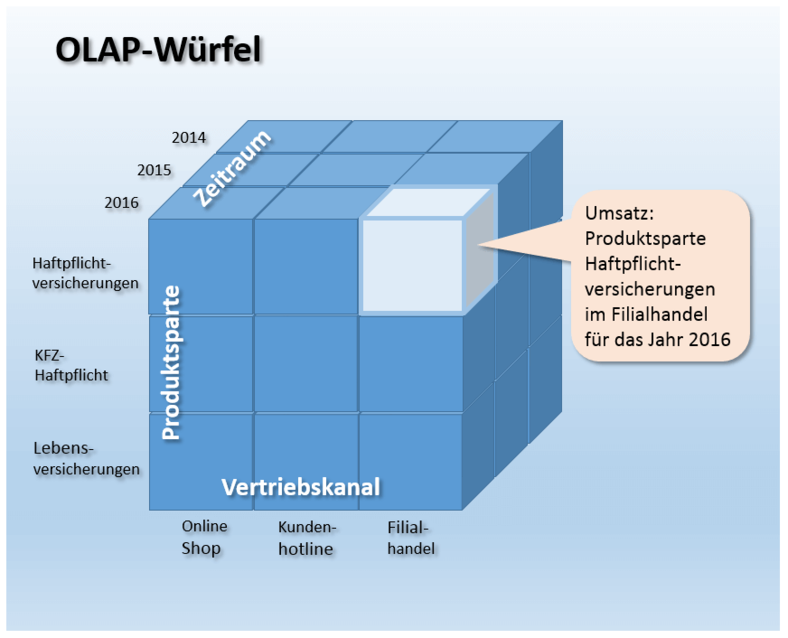
\includegraphics[scale=0.5]{images/OLAP.png}
  \caption[OLAP Cube (01.04.2020)]{OLAP Cube (01.04.2020)}
  \url{https://www.ionos.at/digitalguide/fileadmin/DigitalGuide/Screenshots/schematische-darstellung-eines-olap-wuerfels.png}
  \label{fig:OLAP-Cube}
\end{figure}
\newpage
\subsection{Datenbereitstellungsebene}
Diese Ebene ist die Schnittstelle zwischen Endanwendungen und Präsentationswerkzeugen. Methoden zur Auswertung und Analyse von Daten werden oftmals von diversen Endanwender Tools zur Verfügung gestellt. Diese Tools ermöglichen es, Informationen aus dem Bestand des Data Warehouses zu extrahieren und für den Endanwender in unterschiedlichen Darstellungsformen aufzubereiten. Das Spektrum umfasst Bericht- und Abfragewerkzeuge, \ref{ssec:Bericht-Werkzeug} Kollaborations Tools, \ref{ssec:Kollab-Werkzeug} Data Mining Tools, \ref{ssec:Data-Minging} Werkzeuge des OLAP \ref{ssec:Werkzeuge-OLAP}, und Forecasting- und Simulations Tools \ref{ssec:Forecasting-Tools}.
\subsection{Bericht- und Abfragewerkzeuge}\label{ssec:Bericht-Werkzeug}
Diese Tools ermöglichen es, Endanwender unterschiedliche Funktionen zu benutzen, um vordefinierte Standardberichte erstellen zu können. Diese Berichte können automatisch in einem regelmäßigen Abstand oder nach Abfrage erstellt werden. Um Benutzeranfragen an das Data Warehouse zu erleichtern, kann auf ein Anfrage Assistent Tool zurückgegriffen werden.
\subsection{Kollaborations Tools}\label{ssec:Kollab-Werkzeug}
Durch dieses Tool können die Kommunikation und Zusammenarbeit verschiedener Endbenutzer bei der Datenanalyse unterstützt werden. Einige der Funktionen sind das Speichern von Anmerkungen und der Austausch von Analyseergebnissen.
\subsection{Data Mining Tools}\label{ssec:Data-Minging}
Unter den Begriff Data Mining fallen alle ungerichteten als auch teilweise automatisierten Analysemethoden, die es darauf abgezielt haben, relevante Muster, Trends und Beziehungen im Datenbestand zu ermitteln. Data Mining Tools bauen auf statistische und mathematische Methoden, sowie Techniken aus der Künstlichen Intelligenz (KI) und des Maschinenlernens (ML) auf. Daten, die in Unternehmen für die Analyse eines Data Warehouse erzeugt und verarbeitet werden wachsen exponentiell. Da sich weltweit das durchschnittliche Datenvolumen alle zwei Jahre verdoppelt, gewinnen Data Mining Tools und Methoden im Rahmen des Data Warehousings immer mehr an Bedeutung.
\subsection{Werkzeuge des OLAP}\label{ssec:Werkzeuge-OLAP}
Von allen zur Verfügung stehenden Datenauswertungs- und Datenanalyse Tools haben sich im Rahmen des Datawarehousing vor allem OLAP Anwendungen als Standardbenutzerschnittstelle herauskristallisiert. Tools die im Rahmen des OLAP angewandt werden, stellen Endbenutzer verschiedenste Funktionen zur Verfügung. Mit diesen können Anfragen an das Data Warehouse ad-hoc formuliert werden. Sie dienen als Navigation durch den OLAP Würfel \ref{ssec:Olap-Cube}. 

Die Darstellung in so einem Würfel ermöglicht es, aufbereitete Daten in Abhängigkeit zu beliebig vielen vordefinierten Dimensionen zu modellieren. Um den OLAP Würfel richtig zu bearbeiten gibt es folgende Grundoperationen um dies zu ermöglichen.

\subsubsection{Slicing}\label{ssec:Slicing}
Diese Grundoperation kann eine Dimensionen eines OLAP Würfels auf eine Teilmenge begrenzen. Es wird ein Teil des gesamten Datenbestandes aus dem Datenwürfel herausgeschnitten und separat betrachtet.
\begin{figure}[H]
\centering
  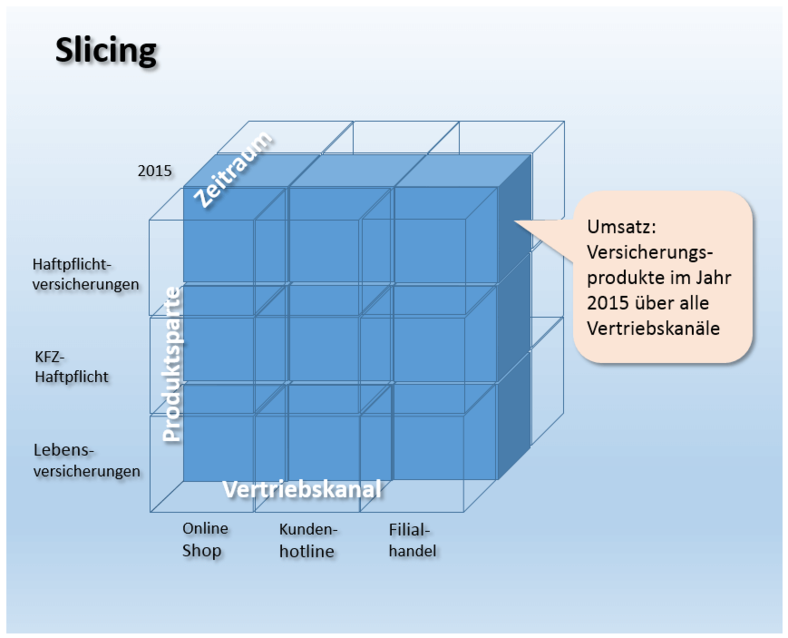
\includegraphics[scale=0.4]{images/Slicing.png}
  \caption[Slicing (01.04.2020)]{Slicing (01.04.2020)}
  {https://www.ionos.at/digitalguide/fileadmin/DigitalGuide/Screenshots/schematische-darstellung-einer-slicing-operation-am-beispiel-eines-dreidimensionalen-olap-wuerfels.png}
  \label{fig:Slicing}
\end{figure}
\newpage
\subsubsection{Dicing}\label{ssec:Dicing}
Wird ein OLAP Würfel durch mehrere Slicing \ref{ssec:Slicing} Operationen in verschiedenen Dimensionen beschnitten, spricht man von Dicing. Wenn Dicing durchgeführt wird, kommt ein kleinerer Würfel als Ergebnis heraus, der eine Teilmenge des Ganzen Würfels darstellt.
\begin{figure}[H]
\centering
  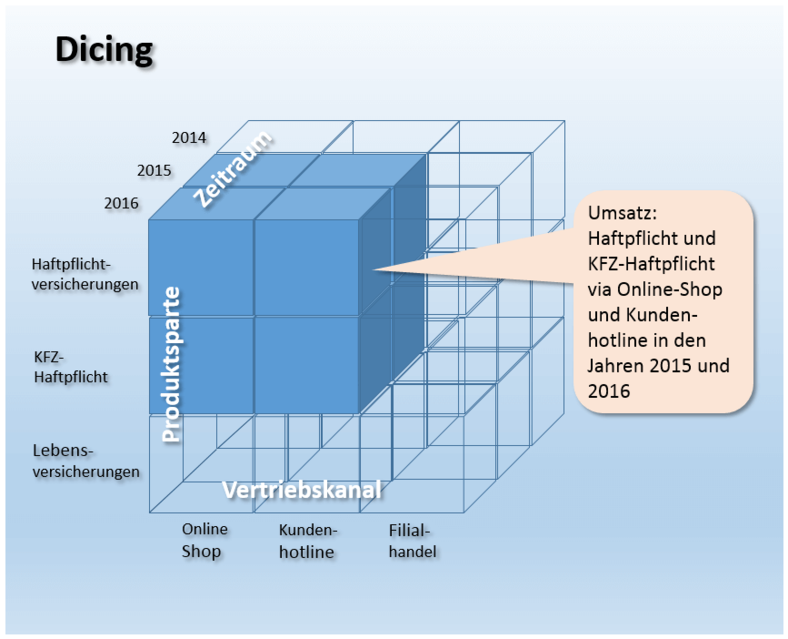
\includegraphics[scale=0.4]{images/Dicing.png}
  \caption[Dicing (01.04.2020)]{Dicing (01.04.2020)}
  {https://www.ionos.at/digitalguide/fileadmin/DigitalGuide/Screenshots/schematische-darstellung-einer-dicing-operation-am-beispiel-eines-dreidimensionalen-olap-wuerfel.png}
  \label{fig:Dicing}
\end{figure}
\newpage
\subsubsection{Pivoting}\label{ssec:Pivoting}
Pivoting ist das Drehen des Würfels. Wenn diese Funktion benutzt wird, wird eine andere Dimension des Gesamtwürfels sichtbar.
\begin{figure}[H]
\centering
  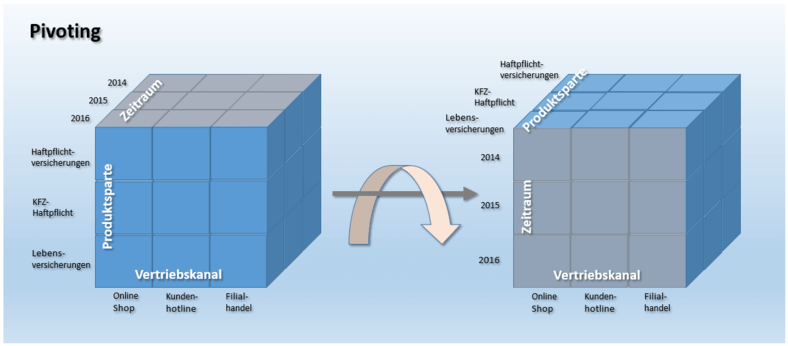
\includegraphics[scale=0.33]{images/Pivoting.png}
  \caption[Pivoting (01.04.2020)]{Pivoting (01.04.2020)}
  {https://www.ionos.at/digitalguide/fileadmin/DigitalGuide/Screenshots/schematische-darstellung-einer-pivoting-operation-am-beispiel-eines-dreidimensionalen-olap-wuerfel.png}
  \label{fig:Pivoting}
\end{figure}
\subsubsection{Drill Down / Roll Up}\label{ssec:Drill-Down}
Sollen die Aggregationen eines Objekts auf detaillierte Werte gebracht werden, kommt die Funktion Drill Down zum Einsatz. Diese Operation ermöglicht es Analysten in einem OLAP Würfel die Daten genauer darzustellen, um somit auch die Granularität der Daten zu erhöhen. Roll Up ist die Gegenoperation von Drill Down. Die Roll Up Funktion verdichtet die Informationen auf höhere Hierachiestufen. Diese beiden Operationen kommen zum Einsatz, um durch eine mehrdimensionale hierarchische Struktur hindurch zu navigieren.
\begin{figure}[H]
\centering
  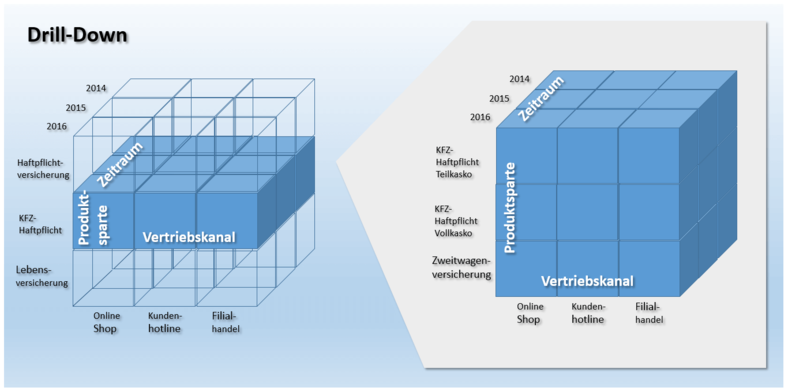
\includegraphics[scale=0.3]{images/Drill-Down.png}
  \caption[Drill Down]{Drill Down}
  {https://www.ionos.at/digitalguide/fileadmin/DigitalGuide/Screenshots/schematische-darstellung-einer-drill-down-operation-am-beispiel-eines-dreidimensionalen-olap-wuerfel.png}
  \label{fig:Drill-Down}
\end{figure}
\subsubsection{Drill Out / Split}\label{ssec:Drill-Out}
Drill Out ermöglicht es Benutzern, einem OLAP Würfel weitere Dimensionen hinzuzufügen. Das Ergebnis dieser Funktion sind detailliertere Daten. Doch anders als bei Drill Down wird der Grad nicht durch die Granularität gewonnen, sonder durch Informationsgewinn. Dieser Gewinn kommt durch die zusätzlichen Referenzinformationen der hinzugefügten Dimension zustande. Die Granularität bleibt erhalten.
\subsubsection{Drill In / Merge}\label{ssec:Drill-In}
Als Gegenoperation zu Drill Out \ref{ssec:Drill-Out} wird der Detailgrad des OLAP Würfels beim Drill In verringert. Dies passiert, indem eine Dimension entfernt wird. Im Gegensatz zu Roll Up kommt der Informationsverlust nicht aus der Veränderung der Betrachtungsebene, sonder durch den Verlust von dimensionaler Information. Auch hier bleibt die Granularität gleich. 
\subsubsection{Drill Across}\label{ssec:Drill-Across}
Diese Operation ermöglicht es auf mehreren OLAP Würfel, globale Analysen durchzuführen. Hier können beliebig viele Faktentabellen mit mindestens einer Dimension analysiert werden. Diese Dimensionen müssen aber die gleiche Hierachiestufe und Granularität aufweisen. 
\subsubsection{Drill Through}\label{ssec:Drill-Through}
In dieser Operation wird eine Zelle des Datenwürfels ausgewählt und im höchsten Detaillierungsgrad betrachtet. Anders als bei Drill Down wird bei Drill Through auf die Quelldaten der Würfelzelle zugegriffen. Das Resultat wird somit aus den Tabellenzellen abgeleitet, die der Berechnung der Würfelzelle zugrunde liegt.
\subsection{Forecasting und Simulations Tools}\label{ssec:Forecasting-Tools}
Diese Tools bieten Endanwendern die Möglichkeit, im Data Warehouse gespeicherte Kennzahlen in die Zukunft fortzuschreiben, um Vorhersagemodelle erstellen zu können. 
\newpage
\subsection{Data Warehouse Management}
In allen Ebenen des Data Warehouses sind spezielle Tools aktiv, die im Bereich Data Warehouse Management zusammengefasst werden. Aufgaben dieser Tools sind der Aufbau, die Wartung und der Betrieb aller Administrationsfunktionen, die im Rahmen des Data Warehousings benötigt werden. Zentrale Aufgaben des Data Warehouse Managements sind das Sicherheitsmanagement sowie das Systemmanagement.
\subsubsection{Scheduling}\label{ssec:Scheduling}
Das Scheduling umfasst die Steuerung der Data Warehouse Prozesse. Administrationsfunktionen im Rahmen des Schedulings lassen sich in Bezug auf die Ebene der Data Warehouse Architektur kategorisieren.
\subsubsection{Datenerfassung / Datenintegration}\label{ssec:Datenerfassung}
Auf der Datenerfassungsebene ist der Data Warehouse Manager für das Design und die Anpassung des ETL-Prozess zuständig. Darüber hinaus werden diese Funktionen bereitgestellt, um Aktualisierungsvorgänge und das Qualitätsmanagement zu überwachen.
\subsubsection{Datenhaltung}\label{ssec:Datenhaltung}
In der Datenhaltung überwachet der Data Warehouse Manager, die Speicherauslastung, konstruiert Aggregationstabellen und führt Archievierungsoperationen und Backupoperationen durch.
\subsubsection{Datenbereitstellung}\label{ssec:Datenbereitstellung}
Administrationsfunktionen auf dieser Ebene umfassen die Benutzerverwaltung als auch die Überwachung von Anfragelaufzeiten. 
\subsubsection{Metadaten Management}\label{ssec:Metadaten-Management}
Die zentrale Komponente des Data Warehouse Managers ist das Metadaten Repository. Dieses enthält alle Informationen, die für die Konstruktionen und den Betrieb des Data Warehouses erforderlich sind, sowie Informationen über den Datenbestand. Im Repository  gespeicherte Metadaten umfassen die Definition des zugrundeliegenden Datenbank Shemas, Informationen zu Speicherstrukturen, Zugriffspfade und Dateigrößen, Metdaten zur Beschreibung der Datenquellen. Auch sind Aktualisierungszeitpunkte, Datenbereinigungs- und Transformationsregeln, Indizes und Partitionstabellen dort hinterlegt. Darüber hinaus sorgt der Data Warehouse Manager für einen Austausch der Metadaten zwischen den einzelnen Komponenten des Data Warehouses. So wird eine homogene Metadatenbasis bereitgestellt.
\subsubsection{Sicherheitsmanagement}\label{ssec:Sicherheitsmanagement}
Das Sicherheitsmanagement umfasst diverse Dienste im Rahmen der Nutzerauthentifizierung. Auch wird die Autorisierung und Verschlüsselung berücksichtigt.
\subsubsection{Systemanagement}\label{ssec:Systemmanagement}
Im Rahmen des Systemmangements stellt der Data Warehouse Manager verschiedene Funktionen für den Betrieb des Data Warehouses bereit. Diese umfassen das Monitoring, die Datenarchivierung oder die Datensicherung.
\section{Was sind Visualisierungs Applikationen [FK]}\label{sec:visualization}
Visualisierungs Applikationen sind eine Möglichkeit Daten als Grafiken widerzuspiegeln. Die Daten können auf vielfältige Art und Weise zusammengestellt werden. Nicht jede Visualisierungs Applikation kann dieselben Datenquellen benutzen und verarbeiten. In Microsoft Word kann man zum Beispiel ausschließlich Microsoft Excel Tabellen für die Diagramme einfügen. In Spezialisierteren Applikationen können weitaus mehr Datenquellen verwendet werden wie Daten direkt aus einer Datenbank auslesen oder mit einer REST [\ref{sec:REST}] Schnittstelle von einem Server zu bekommen.
\subsection{Warum Visualisierungstools}
Viele Unternehmen sammeln täglich riesige Mengen an Daten über ihre Kunden, Mitarbeiter, den Markt und viele andere Dinge, aber dieses Wissen ist einzeln betrachtet in bedeutungslosen Zahlen versteckt.
"Die Datenvisualisierung ermöglicht es, sich bei der Auswertung und Präsentation von Daten auf das Wesentliche zu konzentrieren. Die Entscheidungsfindung lässt sich dadurch erleichtern. Während die Auswertung von Daten, die in reiner Tabellenform vorliegen, aufwendig und zeitraubend ist, sind mit der Datenvisualisierung enorme Zeiteinsparungen realisierbar. Oft ist auf den ersten Blick erkennbar, welche Informationen und Zusammenhänge die Daten bereithalten." (\cite{vorteileDV})
Diese Diagramme können helfen, Marktveränderungen vorherzusagen oder den Gewinn durch intelligente Kostenreduzierung zu erhöhen. 
Dies könnte entweder von einem Betreiber genutzt werden, der ansprechende Diagramme für seine Präsentationen und Berichte verwendet, oder von Datenanalysten, die diese Diagramme studieren und nützliche Informationen ableiten, um Fragen zu beantworten wie "Warum steigt der Markt in Großbritannien, obwohl es den Brexit gibt, und wie können wir das, was in dieser Region funktioniert, in andere Regionen bringen?

\subsection{Visualisierungen in Softwareprodukten}
Nicht nur Marktorientierte Betriebe müssen einen Überblick über ihre Produkte haben, sondern auch Softwareunternehmen oder deren Kunden. Visualisierung kann nämlich auch dazu verwendet werden um Softwareprodukte zu Kontrollieren. Jedes Vernünftige Softwareprodukt gibt eine Menge an Informationen in Form von Log Dateien ab. Der Inhalt von Log Dateien kann alles Mögliche sein von harmlosen Statusmeldungen bis hin zu etwaigen schweren Problemen in Form von Fehlercodes. Fehlercodes wiederum können ebenfalls gänzlich unterschiedlich sein. Ob es ein Problem mit der Hardware gibt das zum Beispiel der Speicher voll ist oder das Netzwerk überlastet ist, Ein Benutzer eine falsche Eingabe ausgeführt hat welche nicht im Programm überprüft wurde oder gar ein Programmfehler der zu einem Absturz geführt hat. Egal welches Problem es ist, man sollte darüber informiert werden und wenn Probleme häufiger auftreten muss man sich darum kümmern. Natürlich gibt es Lösungen die Log Files Manuell auszulesen und den Fehler zu beheben aber es können Probleme öfters vorkommen was nicht sofort auffällt. Was zu dem Punkt führt das es viel einfacher wäre, wenn jeder auf einem Blick sieht wie stark das Netzwerk belastet ist oder wie viele Abfragen es auf einen Server gibt. An dieser Stelle kommen Visualisierungsapplikationen ins Spiel.
\begin{figure}[H]
    \centering
    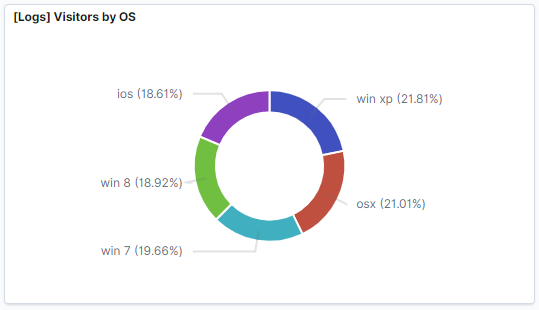
\includegraphics[scale=1.3]{images/sampleLogs1.PNG}
    \caption{Besucher pro Betriebssystem aus Log Dateien}
\end{figure}
\begin{figure}[H]
    \flushleft
    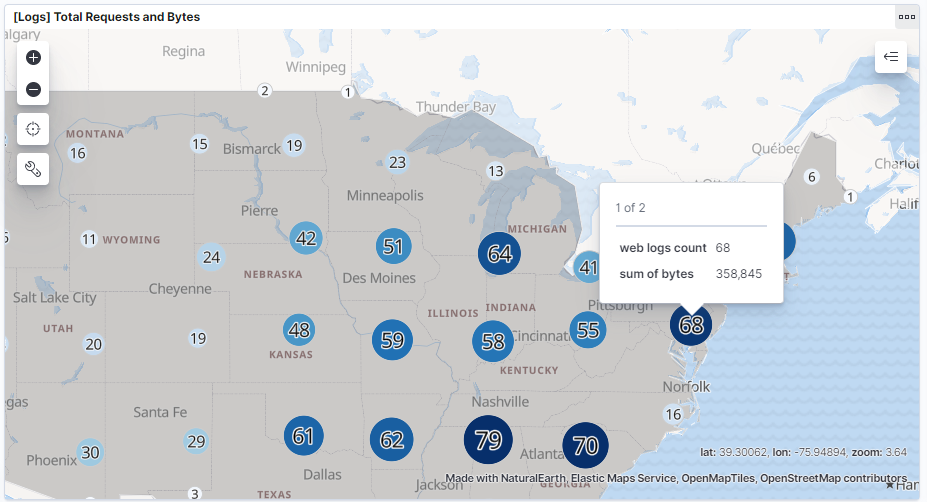
\includegraphics[scale=0.85]{images/sampleLogs2.PNG}
    \caption{Netzwerkverkehr pro amerikanischen Bundesstaat}
\end{figure}
Anhand dieser zwei Beispiele sieht man sehr schön wie nützlich es sein kann seine Daten Live anzusehen. Auf einem Blick sieht man wie hoch die Auslastung in den einzelnen Bundestaaten ist. Somit kann man Maßnahmen ergreifen und zum Beispiel die Serverkapazitäten in den Östlichen Bundesstaaten erhöhen und in den Westlichen verringern, weil dort viel Seltener Anfragen an die Server gestellt werden. Durch gezielteres Lösen von Problemen kann so einiges an Kosten gespart werden. Ein weiterer Großer Vorteil von diesen Visualisierungen ist das Nicht-Techniker die Möglichkeit bekommen auf schnellten Wege an die benötigten Informationen zu kommen und in Meetings einzusetzen. Die Reaktion auf Softwareprobleme kann somit um einiges beschleunigt werden. 

\chapter{Werkzeuge}
\section{Arbeitsumgebung}

\subsection{Portainer[EK]}
\begin{figure}[H]
\centering
  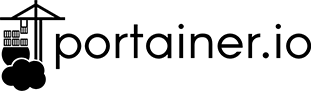
\includegraphics[scale=3]{images/protainer-logo.png}
  \caption{Protainer Logo (02.04.2020)}
  \url{https://pronto-core-cdn.prontomarketing.com/354/wp-content/uploads/sites/2/2018/07/logo-portainer-homepage.png}
\end{figure}
\subsubsection{Allgemein}
Bei portainer.io handelt es sich vereinfacht gesagt um ein Web-UI-Tool, welches ein grafisches Layer über Docker legt. Es handelt sich bei Portainer (Tool und Unternehmung teilen sich den Namen) um eine Open-Source Software, welche sich durch Supportdienstleistungen und spezielle Enterprise-Angebote finanziert.
\vspace{5mm}\par
Durch die GUI wird Zugriff auf die wichtigsten Funktionen von Docker bereitgestellt und bietet darüber hinaus nützliche Features, welche so nicht über die Docker-CLI verfügbar wären. Grundlegender Gedanke hinter so einer GUI ist es die möglichen Fehlerquellen, welche bei einer CLI-Nutzung zu Stande kommen, schnell erkennen zu können. Vor allem bei mehreren Containern kann so der Status durch ein Dashboard im Auge behalten werden, um systemkritische Elemente zeitnah erkennen zu können.
(vgl. \cite{Portainer})
\subsubsection{Entscheidungsprozess}
Von unserem Vorgesetzten der Firma MIC, wurde uns das Tool ans Herz gelegt, da es den Prozess der Problemfindung, durch klare visuelle Marker, in einem Multi-Container-Environment deutlich vereinfacht. 

\subsection{IntelliJ IDEA[EK]}
\begin{figure}[H]
\centering
  
\includegraphics[scale=0.1]{images/intellij_idea_logo.png}
  \caption{IntelliJ IDEA Logo (02.04.2020)}
  \url{https://upload.wikimedia.org/wikipedia/commons/thumb/d/d5/IntelliJ_IDEA_Logo.svg/1000px-IntelliJ_IDEA_Logo.svg.png}
\end{figure}
\subsubsection{Allgemein}
IntelliJ IDEA ist eine von JetBrains entwickelte IDE (zu Deutsch: Integrierte Entwicklungsumgebung). Im Jahre 2001 ins Lebens gerufen, steht IntelliJ heute in zwei Versionen zur Verfügung. Die kostenfreie Open-Source Community-Version wird unter der Apache-2.0 Lizenz vertrieben. Die kostenpflichtige Ultimate-Version wird als Shareware - Testmöglichkeit vor dem Kauf - vertrieben.
(vgl. \cite{IntelliJ-Background})
\subsubsection{Funktionsumfang}
Bei IntelliJ IDEA, handelt es sich um die JVM-IDE der IntelliJ Plattform, daher sind vor allem die JVM Sprachen Java, Scala, Groovy, Kotlin  und gegebenenfalls dazu verwendete Frameworks die Zielgruppe. Es werden aber auch andere Sprachen und Plattformen, wie zum Beispiel TypeScript und Android, unterstützt. Für diese Bereiche gibt es jedoch auch spezielle IDEs, welche auf IntelliJ IDEA basieren. Durch die Analyse des Codes, kann IntelliJ IDEA dem Entwickler Empfehlungen geben - die sogenannte Code-Completion. Die IDE unterstützt durch jenes Wissen den Nutzer bei dem fehleranfälligen Prozess des Refactorings. Neben der Unterstützung während des Schreibens des Codes sind auch Debugger- und Buildtools von Haus aus integriert. Die Erweiterbarkeit ist gegeben; sollten mehr, spezielle oder eigens entwickelte Funktionen benötigt werden, kann dies mittels Plugins gemacht werden.
(vgl. \cite{JetBrains-IDEA})
\subsubsection{Entscheidungsprozess}
Gründe für die Festlegung auf IntelliJ IDEA, war die Tatsache, dass die verwendete Programmiersprache Kotlin und das Build-Automation-Tool Gradle eine solide Integration in IntelliJ IDEA aufweisen. Nachvollziehbar, da die Sprache Kotlin selbst von JetBrains ins Leben gerufen wurden und Gradle ein essenzieller Teil der Kotlin-Idee ist - gezeigt auch dadurch, dass  die Möglichkeit besteht Kotlin-DSLs für die Build-Skripts zu verwenden. Darüber hinaus ist die persönliche Vertrautheit durch die intensive Verwendung dieser IDE in der HTL-Ausbildung durchaus groß, welche das Realisieren neuer Projekte in dieser deutlich fördert.

\subsection{Gradle[EK]}
\begin{figure}[H]
\centering
  
\includegraphics[scale=0.5]{images/gradle-logo.png}
  \caption{Gradle Logo (02.04.2020)}
  \url{https://gradle.org/images/gradle-knowledge-graph-logo.png?20170228}
\end{figure}
\subsubsection{Allgemein}
Gradle ist ein von Gradle Inc. entwickeltes Open-Source Build-Automation-Tool, welches im Jahre 2007 ins Leben gerufen wurde. Über Skripts werden die Build-Instruktionen angeben, diese können mithilfe von Groovy oder Kotlin DSLs geschrieben werden.
Vergleichbar ist Gradle mit Apache Ant und Apache Maven. Bei der Entwicklung von Gradle wurde versucht, die Flexibilität von Ant und das „Build-by-Convention“-Prinzip von Maven zusammenzuführen.
(vgl. \cite{Gradle-Background})
\subsubsection{Was ist ein Build-Automation-Tool?}
Ein Build-Automation-Tool beschreibt eine Anwendung, welche folgende Kriterien erfüllt: 
\vspace{1mm}\par
„Build-Automation ist der Prozess der Automatisierung der Erstellung eines Software-Builds und der damit verbundenen Prozesse, einschließlich dem Kompilieren von Computer-Quellcode in Binärcode, dem Packaging von Binärcode und dem Ausführen automatisierter Tests.“ \cite{Build-Automation}
\newpage
Einfach gesagt helfen Build-Tools dabei, folgende Beispiele zu automatisieren: 
\begin{itemize}
  \item Das Downloaden von Dependencies - Abhängigkeiten - von unserem Code, bei welchem wir zum Beispiel Libraries von Online-Respositories verwenden.
  \item Das Kompilieren vom Source-Code in für uns ausführbaren Code. Wir wollen zum Beispiel, anstatt selbst mit dem Compiler-Tool Kotlin-Code kompilieren zu müssen, diesen Prozess so automatisieren, dass mit einem Kopfdruck unser Code kompiliert und ausgeführt wird.
  \item Das Packaging so zu konfigurieren, dass wir am Ende den Code in der Form haben, welche wir weitergeben wollen. Ein Beispiel dafür wäre, dass wir unseren ganzen Kotlin-Code nach dem Build in einer großen JAR-Datei haben wollen.
  \item Das Ausführen von verschiedensten Tests, zu einem uns passenden Zeitpunkt. Wir wollen zum Beispiel, vor jedem Build sicher stellen, dass die gemachten Änderungen im Code auch noch immer die Kriterien der Unit-Tests erfüllen.
\end{itemize}
Zum Einsatz kommen Build-Tools dann, wenn ein manueller Build-Prozess durch die Anzahl an Dateien nicht mehr unter einem akzeptablen Zeitaufwand möglich ist. Ziel ist es, die Zeit des eigentlichen Entwickelns zu erhöhen.
(vgl. \cite{Gradle-Choice})
\newpage
\subsubsection{Entscheidungsprozess}
\begin{figure}[H]
\centering
  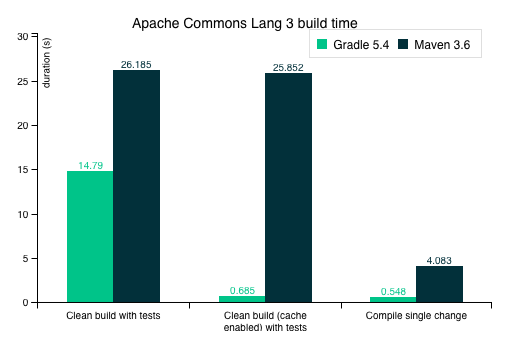
\includegraphics[scale=0.7]{images/gradle-vs-maven.png}
  \caption{Gradle vs. Maven (02.04.2020)}
  \url{https://gradle.org/maven-vs-gradle/}
\end{figure}
Die Entscheidung auf Gradle basiert auf dreierlei Argumenten: Flexibilität, Schnelligkeit und den Wissenserwerb. Die Flexibilität hat vor allem durch den modularen Ansatz dieser Arbeit einen großen Stellenwert. Aus der gezeigten Grafik können wir entnehmen, dass Gradle im Gegensatz zu seinem Pendant Maven beim Aspekt Schnelligkeit einen deutlichen Vorteil vorweist und damit wiederum Wartezeit in der Entwicklung erspart. Wissen in Gradle kann in vielen Softwareprojekten, vor allem größeren, von Nutzen sein - dieser Nutzen setzt jedoch ein bestimmtes Maß an Kenntnis mit diesem Tool voraus.

\subsection{Vim[EK]}
\begin{figure}[H]
\centering
  
\includegraphics[scale=0.2]{images/vim-logo.png}
  \caption{Vim Logo (02.04.2020)}
  \url{https://commons.wikimedia.org/wiki/File:Vimlogo.svg}
\end{figure}
\subsubsection{Allgemein}
Bei Vim handelt es sich sich um einen Command-Line-Editor, welcher mit den meisten Linux-Systemen, wie z.B. Ubuntu, bereits von Haus aus mitgeliefert wird. Ursprünge liegen schon in den 90er-Jahren, vor der Zeit der alltäglichen UI-Interfaces. Vim wird als eine sogenannte Charityware vertrieben, die Software an sich ist kostenfrei und Open-Source, jedoch wird der Nutzer ermutigt, für einen guten Zweck für Kinder in Uganda zu spenden, daher auch der Name Charityware.
(vgl. \cite{Vim-Background})
\subsubsection{Besonderheit}
Die Besonderheit von Vim liegt darin, dass die Idee der Bedienung darauf beruht, alle möglichen Dinge über Kommandos beziehungsweise Shortcuts zu lösen. Der Nachteil für neue Benutzer ergibt sich daraus, dass Vim anfangs überfordernd wirken kann. Dieser Nachteil ist aber auch der größte Vorteil, da sich eine Kenntnis dieser Funktionsweisen, schnell durch einen Geschwindigkeitsgewinn bemerkbar macht.
(vgl. \cite{Vim-Besonderheit})
\subsubsection{Entscheidungsprozess}
Da die verschiedenen Module auf den entsprechenden AWS-Instanzen laufen, fällt wie bei allen Server-Linux-Umgebungen die Möglichkeit einer Benutzung über die UI weg. So benötigt es einen Editor, welcher in dieser Umgebung nicht nur Text anzeigen kann, sondern dem Entwickler auch ein Syntax-Highlighting bietet. Durch Erfüllung dieser Kriterien wurde für Vim im Bereich der AWS-Instanzen zum Editor-of-Choice.

\newpage
\subsection{AWS[AA]}\label{ssec:aws}
\begin{figure}[H]
\centering
  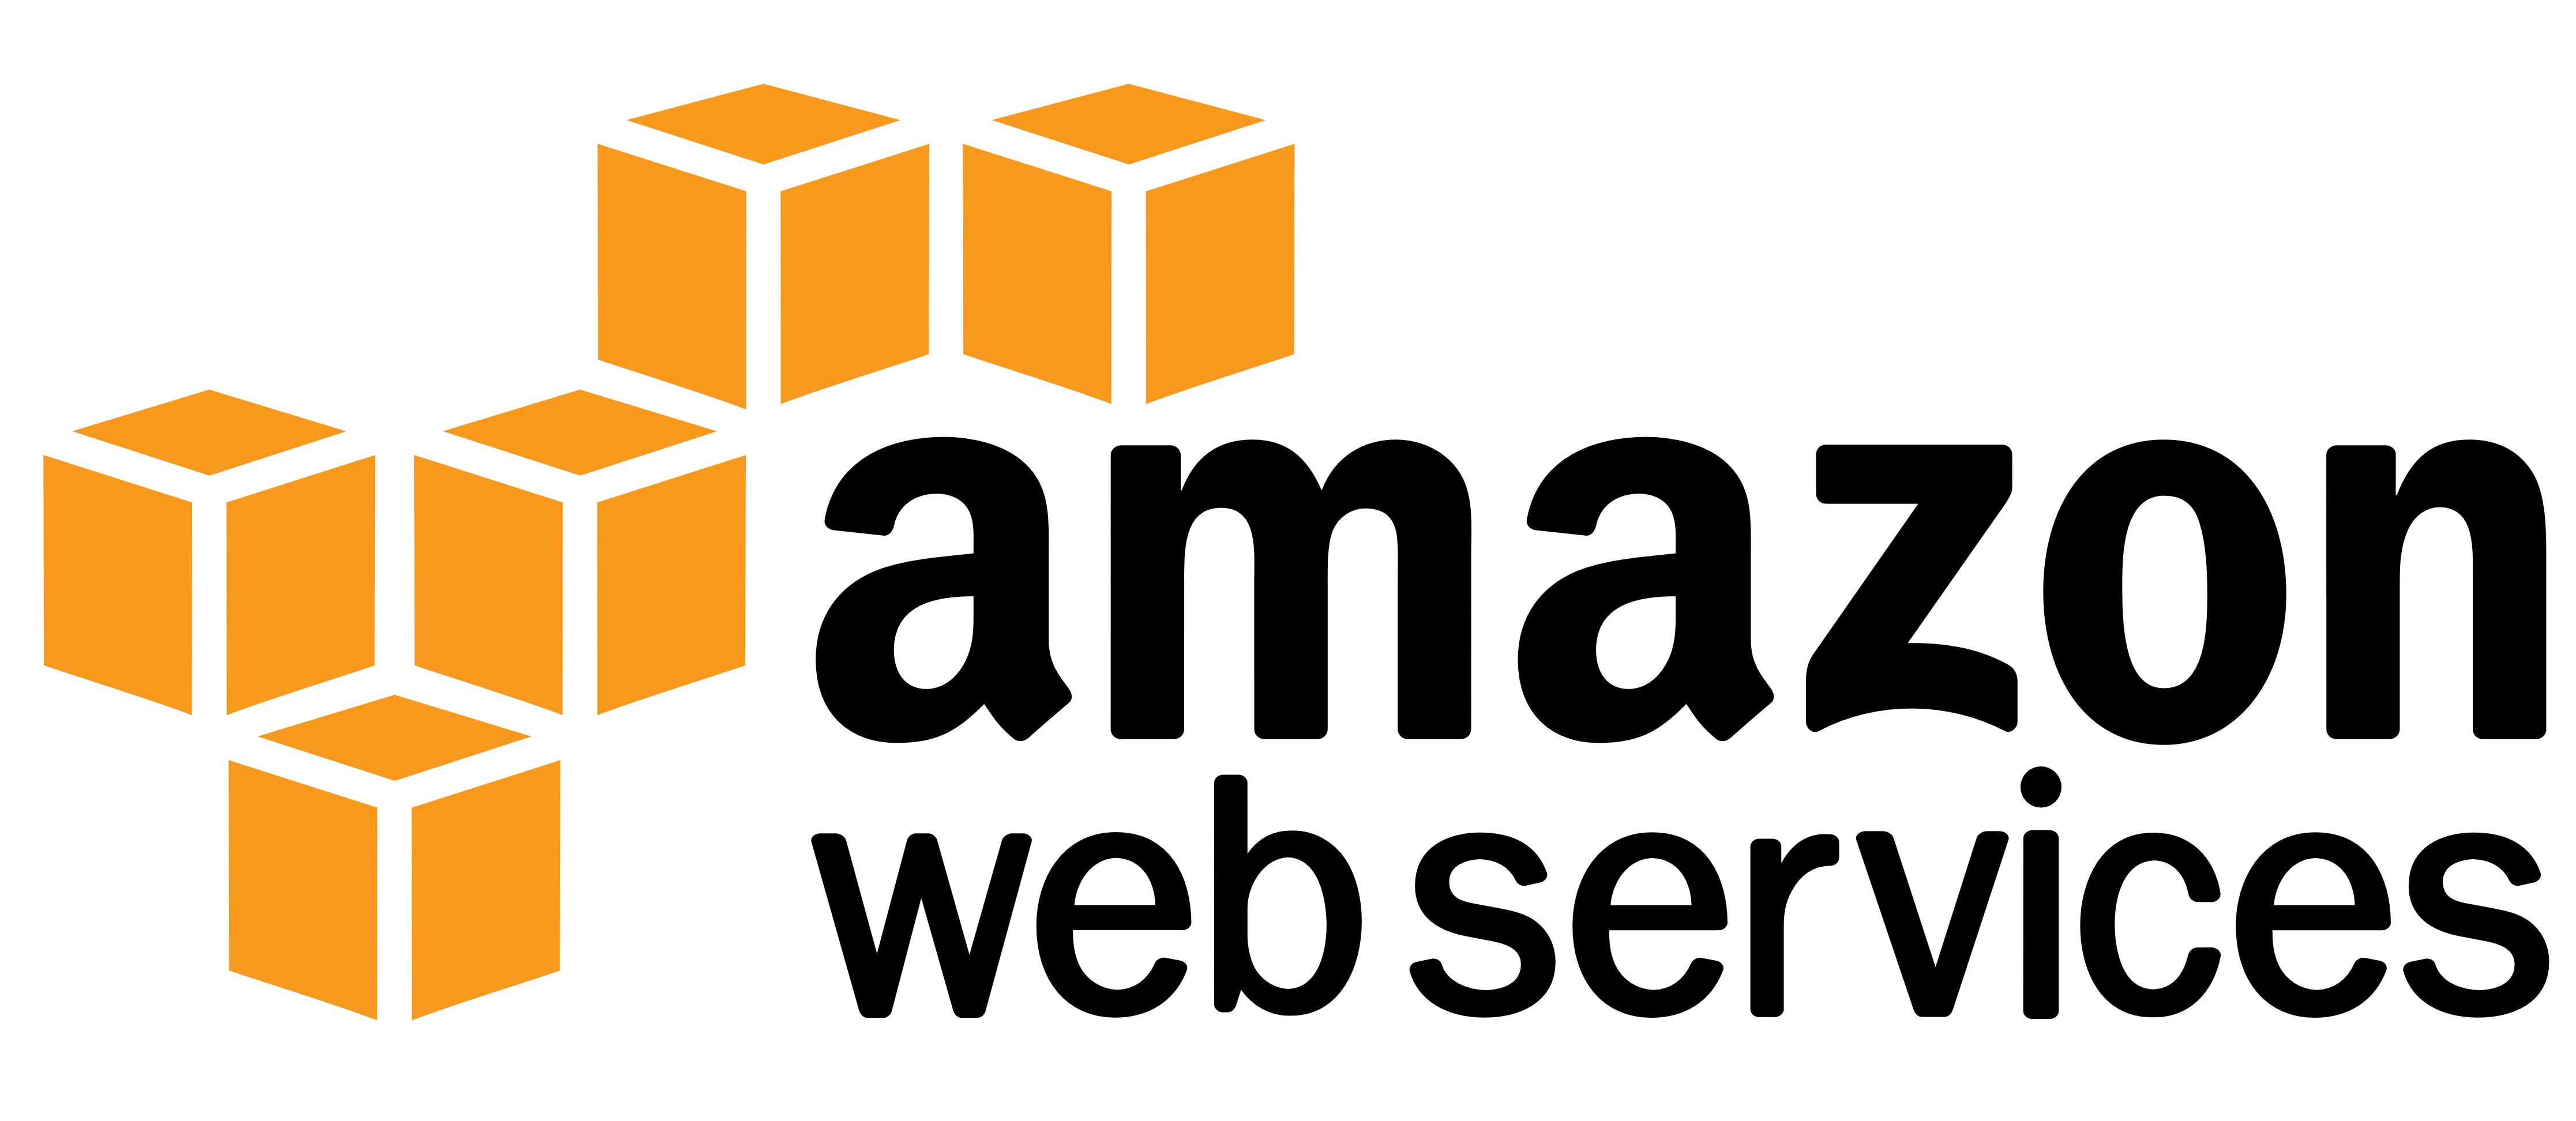
\includegraphics[scale=0.1]{images/aws-logo.png}
  \caption[AWS Logo (01.04.2020)]{AWS Logo (01.04.2020)}
  \label{fig:awslogo}
  \url{https://logos-download.com/wp-content/uploads/2016/12/Amazon_Web_Services_logo_AWS.png}
\end{figure}
Folgende Information wurden aus diesen Quellen herangezogen und überarbeitet.\\ (vgl. \cite{amazon_was_2020} \& \cite{amazon_ec2_2020})
\subsubsection{Allgemeine Beschreibung}
„Amazon Web Services (AWS) ist mit mehr als 175 Services, die umfangreiche Funktionen bieten und in global verteilten Rechenzentren bereitgestellt werden, die weltweit umfassendste und am häufigsten genutzte Cloud-Plattform. Millionen von Kunden – darunter einige der am schnellsten wachsenden Start-up-Unternehmen und der größten Konzerne sowie wichtige Behörden – vertrauen auf AWS, wenn es darum geht, agiler zu werden, Kosten zu senken und Innovationen schneller zu realisieren.“~\cite{amazon_was_2020}
\subsection{EC2}\label{ssec:ec2}
\subsubsection{Allgemeine Beschreibung}
„Amazon Elastic Compute Cloud (Amazon EC2) bietet eine skalierbare Rechenkapazität in der Amazon Web Services (AWS)-Cloud. Amazon EC2 beseitigt die Notwendigkeit, im Voraus in Hardware investieren zu müssen. Daher können Sie Anwendungen schneller entwickeln und bereitstellen. Sie können Amazon EC2 verwenden, um so viele oder so wenige virtuelle Server zu starten, wie Sie benötigen, Sicherheit und Netzwerk zu konfigurieren und den Speicher zu verwalten. Amazon EC2 können Sie auf- oder abwärts skalieren, um auf geänderte Anforderungen oder Datenverkehrsspitzen zu reagieren. Dies reduziert die Notwendigkeit, den Datenverkehr vorauszusagen.“ ~\cite{amazon_ec2_2020}
\newpage
\subsubsection{Funktionen von EC2}
\begin{itemize}
    \item Die primäre Funktion von EC2 sind Instanzen, die virtuelle Datenverarbeitungsumgebungen sind.
    \item Es speichert alle temporären Daten, die gelöscht werden in eigene Volumes, wenn ihre Instanz angehalten beziehungsweise beendet wird. Diese werden als Instanz Speicher Volume bezeichnet.
    \item Es werden bereits von EC2 vorkonfigurierte Vorlagen für Instanzen bereitgestellt. Diese heißen Amazon Machine Images (AMIs), die Komponenten für den Server verpacken können, oder auch Betriebssysteme und zusätzliche Software sein können.
    \item Es können auch Instanz Typen gesetzt werden. Diese beinhalten Konfigurationen für CPU, Arbeitsspeicher und Netzwerkkapazitäten.
    \item Die Anmeldung auf die AWS Maschinen erfolgt durch Schlüsselpaare. AWS selbst speichert den öffentlichen Schlüssel während der Benutzer den privaten Schlüssel speichern muss.
    \item EC2 hat Sicherheitsgruppen die für eine oder mehrere Instanzen benutzt werden können. In diesen wird festgehalten welche Protokolle, Ports und Quell IP Bereiche offen stehen und auf die Instanz zugreifen können.
\end{itemize}
\subsection{Warum AWS EC2?}
\subsubsection{Anforderung von MIC}
Die Anforderung war es die gesamte Systemarchitektur auf der Grundlage von AWS EC2 aufzubauen und dort skalierbar zu machen. Pro Schritt hätte es eine Instanz gegeben, um so mehrere Instanzen, des gleichen Prozesses, zu starten. Der ETL Prozess ist dadurch skalierbar und dynamischer.
\subsection{Probleme}
Durch die Sicherheitsgrundlagen des Unternehmens, war es immer nötig durch Port Forwarding die Ergebnisse der Funktionen an den nächsten Service weiterzuleiten. Denn jeder Port außer der achtziger Port war gesperrt. Deswegen war es immer notwendig, jede Funktion, die das Ergebnis an die nächste Instanz schickte über den achtziger Port gehen zu lassen.\\
Ein anderes Problem mit AWS war die Größe der Maschinen im EC2 Service. Durch die gewaltigen Daten die angekommen sind, war der Speicher der Instanzen oft voll und musste immer erweitert werden. 
\section{Technologien}
\subsection{Databus[EK]}
\subsubsection{Allgemein}
Databus ist ein von LinkedIn entwickeltes Tool, welches sich selbst mit den Attributen „source-agnostic distributed change data capture system“ beschreibt. Als Open-Source Software wurde diese im Jahre 2013 unter der Apache-2.0 Lizenz der GitHub-Community bereitgestellt. 
(vgl. \cite{Databus-GitHub})
\vspace{5mm}\par
\textit{Source-Agnostic} bedeutet, dass Databus im Gegensatz zu einer Spezialisierung auf eine bestimmte Datenquelle, wie zum Beispiel ein bestimmter Typus von Datenbanken, darauf ausgelegt ist, ein breitgefächertes Spektrum an Datenquellen abzudecken. Damit soll die Unabhängigkeit von den Datenquellen gewährleistet werden.
\vspace{5mm}\par
\textit{Distributed} heißt, dass es sich bei Databus um ein verteiltes System handelt, welches sich die Vorteile von mehreren Computersystem zu Nutze machen kann und somit nicht auf ein singuläres System angewiesen ist.
\vspace{5mm}\par
\textit{Change-Data-Capture} (CDC) beschreibt einen Prozess, bei welchem die Änderung in einer Datenquelle - oft einer Datenbank - identifiziert und festgehalten wird. Diese gewonnen Änderungen werden dann an andere Systemarchitekturen, wie zum Beispiel ETL-Prozessen, zur Weiterverarbeitung zur Verfügung gestellt.
(vgl. \cite{CDC})
\newpage
\subsubsection{Wie funktioniert Databus?}
\begin{figure}[H]
    \centering
    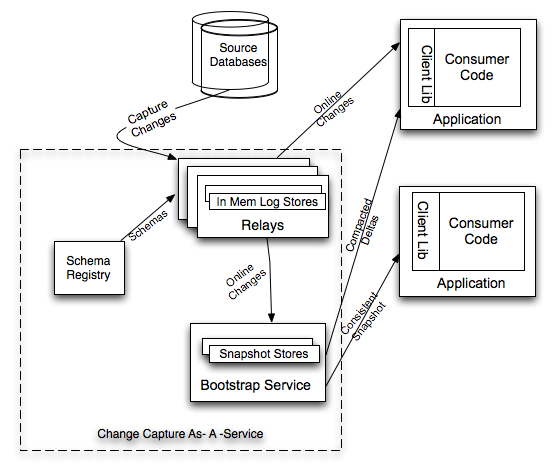
\includegraphics[scale=0.4]{images/databus-as-a-service.png}
    \caption{Databus-Aufbau (02.04.2020)}
    \label{img:}
    \url{http://s3.amazonaws.com/snaprojects/databus/databus-as-a-service.png}
\end{figure}
Wie man in der oben aufgezeigten Grafik sehen kann, besteht Databus aus folgenden drei Teilen: 
\begin{enumerate}
  \item \textbf{Relais:} Nimmt die aufgezeichneten Änderungen in der Datenquelle entgegen. Diese Änderungen werden in einem in-memory Log-Store abgespeichert, da dieser über die nötigen high-performance Eigenschaften verfügt.
  \item \textbf{Bootstrap-Service:} Periodisch nimmt dieser Daten des Relais entgegen. Ermöglicht wird dies durch eine periodische Umlenkung des Relais-Datenstroms auf den Bootstrap-Service. Dieser Service speichert die erhaltenen Daten dann als sogenannten Snapshot - eine Momentaufnahme der Daten zu einem bestimmten Zeitpunkt - ab.
  \item \textbf{Client-Library:} Diese wird in die Applikation eingefügt, um Daten aus dem Relais oder Bootstrap-Service erhalten zu können.
\end{enumerate}
Sollte der Fall eintreten, dass ein Consumer - eine Applikation, welche die Client-Library verwendet - datentechnisch zeitlich zurückfällt, so dass die benötigten Daten im Relais nicht länger vorliegen, kommt es zu folgendem Fall: ein konsolidierter Snapshot wird dem zurückliegenden Consumer übergeben, welcher diesen wieder auf Kurs bringt. Ähnlich sieht der Fall aus, wenn sich einer neuer Consumer einklinkt. Der Bootstrap-Service stellt auch in diesem Fall einen Snapshot bereit, welcher es dem Consumer ermöglicht, auf den aktuellen Stand zu kommen.
(vgl. \cite{Databus-Open-Sourcing})
\subsubsection{Entscheidungsprozess}
In der ersten Phase der Arbeit, sozusagen der Aneignungsphase, war Databus noch im Technologie-Stack enthalten. Anfangs wirkte das Tool vielversprechend für die Firma, durch Aspekte wie die freie Verfügbarkeit als Open-Source Software und damit die Möglichkeit eines Einblicks in dessen Funktionsweise. Doch bei weiterer Einarbeitung und Kenntnisnahme über die genaue Funktionalität, wurde die Verwendung von Databus auf Eis gelegt. Für die Firma MIC ist die Tatsache, dass man für die Verwendung von Databus jede Tabelle, welche auf Änderung beobachtet wird, abändern muss, ein Problem. Der Grund dafür liegt an der Menge der Tabellen, welche abgeändert werden müssten und dass ein solches Vorgehen nicht dem Echtzeitbetrieb vereinbar ist.

\subsubsection{Die Problematik verwahrloster Open-Source Software}
Wenn eine zuvor intern in Unternehmen entwickelte Software den Schritt macht, in den Open-Source Bereich entlassen zu werden, dann oft mit der Hoffnung, durch größere Beteiligung der Community und auch anderer Unternehmungen am Ende eine bessere Software zu erhalten, als wenn diese inhouse entwickelt worden wäre.
\vspace{5mm}\par
Dies beschreibt allerdings nur den Optimalfall. Durch die schnellen Veränderungen in einer Branche wie dieser kann es schnell zu Problemen bei der Nutzbarkeit der Software kommen, wenn diese nicht regelmäßig gewartet wird.So auch der Fall bei Databus, selbst die Replikation der auf GitHub präsentierten Beispiele war nur durch externe fremdsprachige Ressourcen möglich. Somit ist ein deutlich größerer Zeitaufwand  nötig, welcher nur schwer im voraus zu kalkulieren ist. Ohne also eine große Code-Kenntnis der Software kann ein solches Unterfangen schnell zu einer Gefahr werden, wenn längerfristig Projekte darauf aufgebaut werden sollen. 
\newpage
\subsection{Kafka[EK]}
\begin{figure}[H]
    \centering
    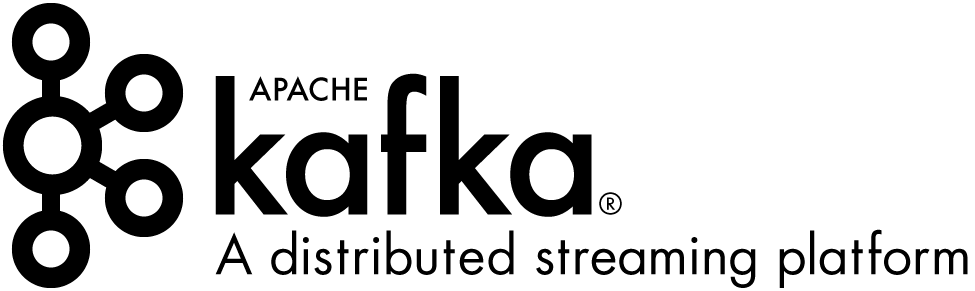
\includegraphics[scale=0.4]{images/kafka_logo.png}
    \caption{Kafka Logo (02.04.2020)}
    \url{https://kafka.apache.org/images/logo.png}
\end{figure}
\subsubsection{Allgemein}
Bei Kafka handelt es sich um eine verteilte Streaming-Plattform, welche von LinkedIn im Jahre 2011 als Open-Source Projekt veröffentlicht wurde. 
(vgl. \cite{Kafka-Open-Sourcing})Durch den Apache Incubator kam das Projekt im Jahre 2012 in die Hände der Apache Software Foundation und wird seitdem auch von Apache weiterentwickelt und gewartet.
(vgl. \cite{Kafka-Apache-Incubator})
\vspace{5mm}\par
Als Streaming-Plattform deckt Kafka drei Funktionalitäten ab.
Erste wäre das Ver-öffentlichen und Abonnieren von Record-Streams (Kafkas Bezeichnung für einen Datenstrom), ähnlich zu einem Enterprise-Messaging-System (EMS). Zweite wäre das Speichern von solchen Record-Streams, in einer Weise, in welcher diese dauerhaft fehlertolerant erfolgen. Dritte wäre die Verarbeitung von Streams im Moment des Auftretens.
\vspace{5mm}
Kafka soll vor allem diesen zwei Klassen von Applikationen zur Seite stehen:
\begin{itemize}
    \item Echtzeit Streaming-Data-Pipelines, welche zuverlässig Daten zwischen System oder auch Applikationen transportieren.
    \item Echtzeit Streaming-Applikationen, welche auf Daten-Streams reagieren oder diese transformieren.
\end{itemize}
(vgl. \cite{Kafka-Introduction})

\subsubsection{Wie funktioniert Kafka?}
Kafka wird als ein sogenannter Cluster auf einem oder mehreren Servern ausgeführt. 
\vspace{5mm}\par
Ein Cluster ist: „Eine Gruppe von unabhängigen Servern (üblicherweise in unmittelbarer Nähe zu einander), welche durch ein dediziertes Netzwerk vernetzt als eine zentralisierte Datenverarbeitungsressource arbeiten“
\cite{Cluster-Definition}
\newpage
Dieser Cluster speichert dann die Record-Streams in sogenannten Topics - die Kategorien für die Aufzeichnungen. Jede dieser Aufzeichnungen beziehungsweise Records steht aus dreierlei Bestandteilen: dem Key (eindeutige Identifikation), dem dazugehörigen Value (Wert) und einem Zeitstempel. Für das Management dieser Cluster verwendet Kafka Zookeeper.
\begin{figure}[H]
    \centering
    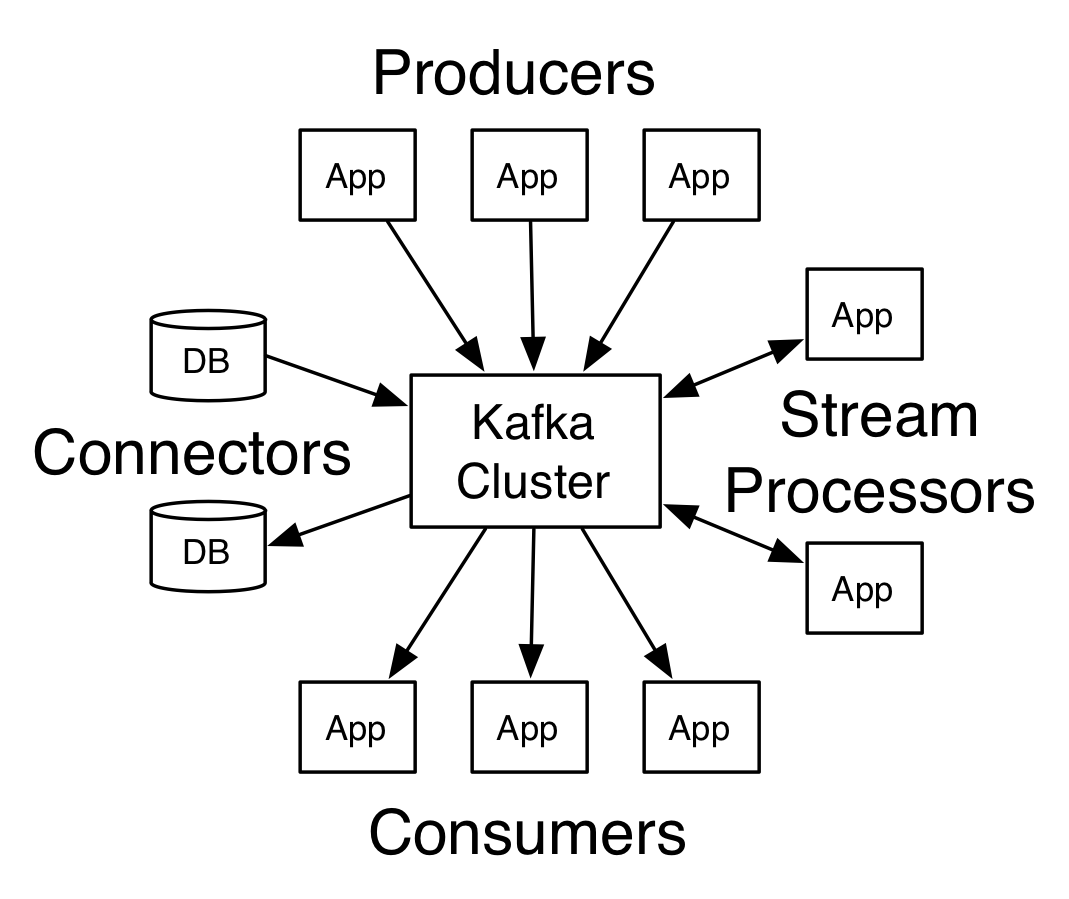
\includegraphics[scale=1.5]{images/kafka-apis.png}
    \caption{Kafka APIs (02.04.2020)}
    \url{https://kafka.apache.org/23/images/kafka-apis.png}
\end{figure}
Wie in der vorhergehenden Grafik zu sehen ist, bilden vier Core-APIs Kafka:
\begin{enumerate}
  \item \textbf{Producer API:} Will eine Applikation einen Record-Stream an den Kafka-Cluster und damit an ein Topic senden, so kann sie dies über diese API lösen.
  \item \textbf{Consumer API:} Bildet das Gegenstück zur Producer API; will eine Applikation zu einem bestimmten Topic zugehörige gesendete Record-Streams haben, muss jene einfach dieses Topic abonnieren.
  \item \textbf{Stream API: } Nimmt die beiden vorangegangen API-Funktionen Eins und Zwei an. Somit kann eine Applikation als ein Stream-Prozessor agieren, welcher sowohl den Input-Stream eines Topics konsumiert, als auch den Output-Stream zu einem anderen Topic liefert. So kann diese API einen Input-Stream zu einem Output-Stream transformieren.
  \item \textbf{Connector API:} Soll die Möglichkeit, geben bereits vorhanden Systeme und Applikationen mit einem Kafka-Topic zu verbinden, dies kann einerseits als Consumer und andererseits auch als Producer erfolgen. Ein Beispiel für einen Producer  wäre, wenn jede Änderung einer Datenbanktabelle aufgezeichnet werden soll und über den Kafka-Cluster für eine Weiterverarbeitung bereitstehen soll.
\end{enumerate}
Die APIs erlauben darüber hinaus, nicht nur die Verarbeitung eines Topics. Alle beschriebenen Funktionalitäten sind auch mit mehreren Topics möglich.
(vgl. \cite{Kafka-Introduction})
\subsubsection{Entscheidungsprozess}
Die Echtzeit-Komponente von Kafka ist ein tragender Grund für die Verwendung in dieser Arbeit, dies ermöglicht den Komponenten ohne größeren Zeitverlust die weiterzugebenden Daten mit der nachfolgenden Komponente zu kommunizieren. Des weiteren handelte es sich bei Kafka um eine Vorgabe der Firma MIC.

\subsection{ZooKeeper[EK]}
\begin{figure}[H]
    \centering
    
\includegraphics[scale=0.25]{images/zookeeper-logo.png}
    \caption{ZooKeeper Logo (02.04.2020)}
    \url{https://upload.wikimedia.org/wikipedia/en/thumb/8/81/Apache_ZooKeeper_Logo.svg/403px-Apache_ZooKeeper_Logo.svg.png}
\end{figure}
\subsubsection{Allgemein}
ZooKeeper ist eine Open-Source Software, welche von Freiwilligen unter dem Dach der Apache Software Foundation entwickelt wird. Ziel des Projektes ist es, einen Server, der eine sehr zuverlässige Koordination von verteilten System ermöglicht, bereitzustellen. 
(vgl. \cite{Apache-ZooKeeper})
\subsubsection{Nutzen für Kafka}
Beim Management der Cluster für Kafka fallen die folgenden Aufgaben an ZooKeeper. Die Koordinierung von Brokern. Das Bereitstellen von einem konsistenten Dateisystems für die Konfigurationsdateien. Die Auswahl eines sogenannten „Broker Topic Partition Leaders”.
(vgl. \cite{Kafka-Architecture})

\subsubsection{Funktionsweise}
Die interne Datenstruktur von ZooKeeper ähnelt einem Baum, heißt von dem Ausgangspunkt beziehungsweise der Wurzel erreichen wir alle weiteren Elemente über eine direkte Verbindung oder über deren übergeordneten Elemente. Jedes Element in diesem Baum ist ein Knoten, eine sogenannte zNode (z steht für Zookeeper, Node ist der englische Begriff für Knoten). Ein Beispiel dafür ist in der folgenden Grafik zu sehen.
\begin{figure}[H]
    \centering
    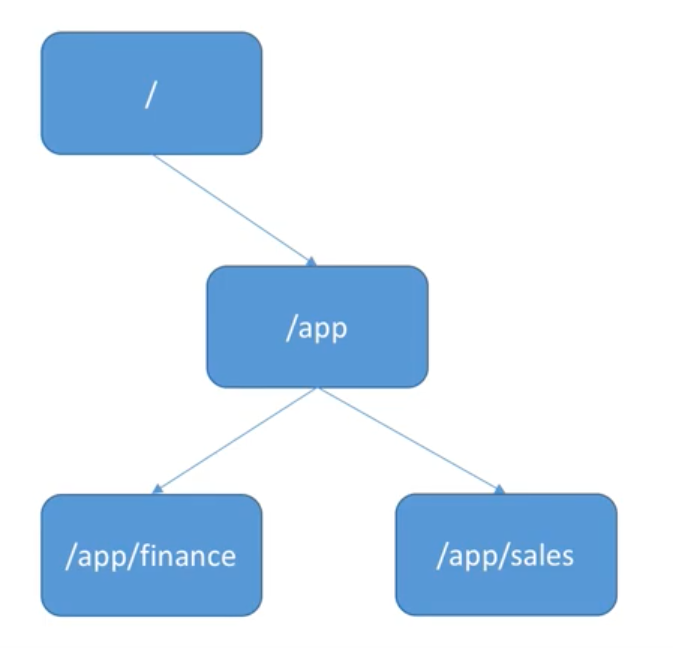
\includegraphics[scale=0.3]{images/zookeeper-node.png}
    \caption{ZooKeeper zNodes (02.04.2020)}
    \url{https://youtu.be/AS5a91DOmks?t=161}
    \label{img:}
\end{figure}
Die Eigenschaften einer zNode sind, dass jede über einen Pfad verfügt und entweder persistent oder ephermal sein kann - Kafka verwendet beide. Mit persistent ist gemeint, dass die zNode immer existiert, also somit eine persistente Präsenz aufweist. Die ephemeral zNode ist nur zur Zeit der Verbindung mit der Applikation existent. Darüber hinaus kann eine zNode Daten speichern, kann nicht umbenannt werden und bietet die Möglichkeit für eine Observierung. Heißt, dass sich Abonnenten dieser zNode darüber informieren lassen können, ob eine Änderung in dieser stattgefunden hat.
(vgl. \cite{ZooKeeper-Video})
\subsubsection{Entscheidungsprozess}
Als ein Bestandteil von Kafka, fällt eine jede direkte Entscheidung weg, da eine Entscheidung für Kafka immer auch eine für Zookeeper ist.

\subsection{Kotlin[EK]}
\begin{figure}[H]
    \centering
    
\includegraphics[scale=0.1]{images/kotlin-logo.png}
    \caption{Kotlin Logo (02.04.2020)}
    \url{https://upload.wikimedia.org/wikipedia/commons/thumb/7/74/Kotlin-logo.svg/1024px-Kotlin-logo.svg.png}
\end{figure}
\subsubsection{Allgemein}
Bei Kotlin handelt es sich um eine relativ neue Sprache, welche im Jahre 2011 von JetBrains ins Leben gerufen wurde. Als Open-Source Sprache ist diese nicht allein von JetBrains abhängig, seit Google sie im Jahre 2017 als die neue offizielle Sprache für Android über Java ernannt hat. Folgend stiegen auch sie bei der Entwicklung ein. Darüber hinaus, wie bei den meisten Open-Source Projekten, beteiligt sich auch die Community an der Entwicklung der Sprache. Ziel der Sprache ist die Multiplattform. Kotlin-Code ist damit nicht nur auf der JVM lauffähig, sondern auch Native und im Web. Gemeinsam bilden Google und JetBrains die Kotlin Foundation.
\subsubsection{Merkmale}
\begin{itemize}
  \item \textit{Kurz und prägnant.} Ein sogenanntes POJO mit Gettern, Settern und Standardfunktionen, wie „toString()“ können in einer Zeile geschrieben werden. Lamda-Expressions erlauben Operationen, wie zum Beispiel das Filtern einer Liste, ohne viel Boilerplate-Code. 
  \item  \textit{Typsicherheit und keine NullPointer-Exceptions.} Kotlin ist eine stark und statisch typisierte Programmiersprache. Eine Variable für den Compiler darf nicht den Wert null annehmen, außer dies wird explizit angegeben. Bei einer Typenprüfung wird die Variable automatisch gecastet und erlaubt somit den direkten Zugriff auf die typenspezifischen Felder, Eigenschaften und Funktionen.
  \item  \textit{Interoperabel.} Kotlin kann, je nach Target-Plattform, auf die existierenden Öko-systeme zugreifen. So kann in der JVM-Plattform die große Vielfalt an existierenden Libraries genutzt werden.
\end{itemize}
(vgl. \cite{Kotlin-Lang})
\subsubsection{Syntax}
Da in Kontext dieses Projekts Kotlin vor allem als Ersatz für Java eingesetzt wird, wird hier die Syntax im Vergleich zu Java erläutert. Dies heißt, das auf Unterschiede eingegangen wird, welche vor allem der Veranschaulichung der Argumentation für den Entscheidungsprozess dienen soll.
\begin{lstlisting}[caption={Kotlin-Hello-World}, language=Kotlin]
fun main() {
    println("Hello world!")
}
\end{lstlisting}
\vspace{4mm}\par
Wie auch in Java ist die Main-Funktion der Einstiegspunkt der Applikation. Bereits jetzt wird im Beispiel ersichtlich, dass mit deutlich weniger Zeilen das klassische Hello-World-Programm geschrieben werden kann. In Kotlin darf auf die in Java obligatorische Klasse verzichtet werden; Funktionen werden im Unterschied mit dem Kürzel „fun“ deklariert. Es entfallen auch die Einstiegsargumente, welche bei Bedarf jedoch angegeben und verwendet werden können. Es entfällt in den meistens Fällen auch das Semikolon „;“. 
Hier der gleiche Code in Java:
\begin{lstlisting}[caption={Java-Hello-World}, language=Kotlin]
class HelloWorld {
    public static void main(String[] args) {
        System.out.println("Hello, World!"); 
    }
}
\end{lstlisting}
\vspace{4mm}\par
Im Bereich der Variablen bietet Kotlin alle bereits bekannten Datentypen, auch gibt es die Möglichkeit spezielle Datentypen über Java-Libraries zu nutzen. Im Unterschied zu Java muss der Datentyp nicht zwingend angeben werden, wenn der Compiler dies aus dem Kontext lesen kann. Hier die Möglichkeiten eine Variable zu deklarieren:
\vspace{3mm}\par
\newpage 
\begin{lstlisting}[caption={Val \& Var}, language=Kotlin]
val a: Int = 1
val b = 2
val c: Int 
var d = 3
\end{lstlisting}
\vspace{4mm}\par
An erster Stelle der Deklaration gibt die Art der Variable an, dies kann val oder var  sein. Val definiert eine read-only Variable. Bei Var hingegen handelt es sich um ein Variable, welche jederzeit, konform nach ihrem Datentyp, neu zugeordnet werden kann. 
Beim Wert c können wir sehen, dass der Compiler zu dieser Zeit noch nicht wissen kann, um welchen Datentyp es sich handelt, aus diesem Grund muss dieser explizit angegeben werden.
Eine weitere Besonderheit von Kotlin ist, dass ein „if“ auch als Expression fungieren kann, dies sieht wie folgt aus:
\vspace{3mm}\par
\begin{lstlisting}[caption={if-Expression}, language=Kotlin]
c = if (a > b) a else b
\end{lstlisting}
\vspace{4mm}\par
Hiermit wird immer die größere Zahl von a und b auf c zugewiesen.
(vgl. \cite{Kotlin-Basic-Syntax})
\subsubsection{Entscheidungsprozess}
Die Möglichkeiten wären Java, Python und Kotlin gewesen. Kotlin wurde als Sprache gewählt, da vor allem die schnelle Entwicklung von den Eigenschaften, wie weniger Boilerplate und dem Wegfallen der Nullpointer-Exceptions, profitiert. Dies sind aber vor allem persönliche Präferenzen, welche auch mit anderen Sprachen hätten erreicht werden können. Schlagkräftiges Argument war die Interoperabilität mit Java, da die Firma auf einer großen Java-Codebase sitzt. Wissen von Java kann daher schnell in Kotlin angewandt werden. Die Kompaktheit des Codes in Kotlin und der Möglichkeit auf Java-Code und deren Libraries zurückzugreifen unterstützte die Wahl.

\newpage
\subsection{NoSql Datenbanken [AA]}
Folgende Informationen wurden aus nachstehender Quelle bezogen. (vgl. \cite{bigdata_nosql_2020})
\subsubsection{Allgemeine Beschreibung}
NoSQL steht für Not only SQL und beschreibt Datenbanksysteme, die einen nicht-relationalen Ansatz haben. Datenbanken, die diesem Modell zugrunde liegen, sind horizontal skalierbar und lassen sich für Big-Data-Anwendungen einsetzen. Da NoSQL, Not only SQL bedeutet kann man nicht grundsätzlich auf die Datenbanksprache SQL (Structured Query Language) verzichten. Viele dieser Systeme setzen zwar komplett auf nicht relationale Funktionen, doch existieren auch NoSQL Datenbanken, die nur bestimmte Elemente von SQL-Systemen unberücksichtigt lassen.\\

Während relationale Datenbanken Tabellen mit Zeilen und Spalten für die Datenspeicherung verwenden, nutzen NoSQL Datenbanken zum Beispiel Objekte, Dokumente, Liste etc. für die Organisation der Daten. Diese Systeme haben eines gemeinsam, dass sie optimiert sind für Aufgaben, bei denen SQL Systeme an ihre Grenzen stoßen.\\

Aufgrund des Aufbaus skalieren NoSQL-Datenbanken horizontal. In vielen Fällen sind dies Open Source Softwares, doch gibt es einige Ansätze, die auf eine kommerzielle Lösung basieren. Durch das Fehlen eines Schemas, sind NoSQL Systeme flexibel einsetzbar und eigenen sich für große Datenmengen, wie sie aus Big Data Anwendungen kommen. Die Architektur ist auf Skalierbarkeit und Performance ausgelegt. Fast alle NoSQL Ansätze und Modelle lassen sich in vier Hauptkategorien einteilen. Diese sind Key-Value Datenbanken. Dokumentenorientierte Datenbanken, Spartenorientierte Datenbanken und Graphen Datenbanken.\\

Folgende Eigenschaften zeichnen die NoSQL Systeme aus: das Vermeiden unnötiger Komplexität, eine hohe Performance, die horizontale Skalierbarkeit, die Vermeidung von relationalen Ansätzen des Datenmappings, die Unterstützung der aktuellen Hardwaregenerationen und die Einfachheit in der Installationen und Konfiguration von verteilten Clustern.
\newpage
\subsection{Dokumentenorientierte Datenbanken}
Für diese Informationen wurde auf folgende Quelle zurückgegriffen. (vgl. \cite{ionis_dokumentenorientierte_2020})
\subsubsection{Allgemein}
Dokumentorientierte Datenbanken oder auch Document Stores genannt, finden Verwendung in der Verwaltung von semistrukturierten Daten. Mit semistrukturierten Daten sind Daten gemeint, die keine feste Struktur haben, sondern die Struktur selbst aus den Daten hervorgeht. Durch die fehlende klare Struktur in den Daten sind diese nicht für relationale Datenbanken geeignet, da sich die Informationen nicht in Tabellen einordnen lassen.\\

Die Datenbank erstellt dann einen Schlüssel zu jedem Dokument damit alles zugeordnet ist. Im Dokument selbst, dass zum Beispiel mit JSON, YAML oder XML formatiert ist sind die eigentlichen Daten gespeichert. Da die Datenbank kein bestimmtes Schema hat, kann man auch verschiedene Dokumenttypen gemeinsam in eine Dokumentorientierte Datenbank einbinden. Änderungen der Daten in den Dokumenten müssen nicht der Datenbank mitgeteilt werden.\\
 
Daten unterschiedlichster Formate und ohne gemeinsames Schema können in ein Document Store untergebracht werden. In der Praxis wird in der Regel nur ein Dateiformat für die Dokumente verwendet. Anschließend wird durch die Informationen eine feste Struktur aufgebaut. Durch diese festgelegten Regeln ist es einfacher die Daten zu verarbeiten zusätzlich wird die Arbeit mit der Datenbank verleichtert. Aufgrund dieser Ordnung können Suchanfragen an die Datenbank viel besser verarbeitet werden. In einer dokumentbasierten Datenbank können die gleichen Aktionen durchgeführt werden wie auch in einer relationalen Datenbank. Daten lassen sich einfügen, löschen, abfragen und ändern.\\
 
Damit sich diese Aktionen durchführen lassen, erhält jedes einzelne Dokument einen eindeutigen Schlüssel. Wie dieser Schlüssel zusammengesetzt wird, ist im Grunde egal. Eine einfache Zeichenfolge, der komplette Pfad oder andere Methoden können genutzt werden um das Dokument zu adressieren.
\newpage
\subsubsection{Mongo DB}\label{ssec:MongoDB}
\begin{figure}
\centering
	
\includegraphics[scale=0.05]{images/MongoDB.png}
	\caption[MongoDB (01.04.2020)]{MongoDB (01.04.2020)}
	\url{https://cdn.worldvectorlogo.com/logos/mongodb.svg}
	\label{fig:sample}
\end{figure}
Als Grundlage nachstehender Informationen dienten folgende Quellen. (vgl. \cite{mongodb_beliebteste_2020} \& \cite{scale_cassandra_2020} \& \cite{jepsen_jepsen_2020})
\paragraph{Allgemein}\mbox{} \\	
„MongoDB ist eine universelle, dokumentbasierte, verteilte Datenbank für die moderne Anwendungsentwicklung und die Cloud, die in puncto Produktivität höchsten Ansprüchen gerecht wird.“~\cite{mongodb_beliebteste_2020}

\paragraph{Expressive Object Model}\mbox{} \\
MongoDB unterstützt ein ausdrucksstarkes Objekt Modell. Objekte in der MongoDB können Eigenschaften haben und in sich selbst verschachtelt sein. Ein Objekt kann also mehrere Stufen haben. Dieses Modell ist sehr objektorientiert und kann jede Objektstruktur leicht repräsentieren. Außerdem kann jedes Objekt indexiert werden, noch dazu auf jeder Stufe.
\paragraph{Sekundäre Indizes}\mbox{} \\
Dieses Konzept vereinfacht es jede Eigenschaft eines Objekts zu indexieren egal, ob es verschachtelt ist oder nicht. Dadurch wird es einfacher diese Indizes abzufragen und die Ergebnisse davon zu erhalten.
\paragraph{Hohe Erreichbarkeit}\mbox{} \\
Die Datenbank unterstützt ein Single Master Model. Das bedeutet, dass es einen Eltern Knoten und viele Kinder Knoten gibt. Falls der Eltern Knoten ausfällt oder einfach nicht mehr funktioniert wird ein Kind der neuen Eltern Knoten. Früher benötigte dieser Prozess, 10 bis 40 Sekunden, aber seit neuesten wird alles unter 2 Sekunden geregelt. Während der Zeit bis ein neuer Elternknoten gefunden wird, rennt das Replika Set nicht und nimmt keine Schreibbefehle an. \\
\newpage
\paragraph{Schreib Skalierbarkeit}\mbox{} \\
MongoDB kann mit seinem Single Master Model nur auf seinen Primären Server Schreibbefehle annehmen. Während die sekundären Server nur für Lesebefehle benutzt werden. Wenn die Datenbank drei Replika Sets hat kann nur der Eltern Knoten Schreibbefehle entgegennehmen, während die Kinder nur Lesebefehle ausführen können. Dies schränkt die Skalierbarkeit sehr ein. Hierfür können aber alle Knoten gestriped werden, damit jeder einzelne Knoten Lese- beziehungsweise Schreibbefehle entgegen nehmen kann.
\paragraph{Query Language Support}\mbox{} \\
Die Datenbank hat eine eigene Query Language, kann aber auch ANSI SQL unterstützen.
\paragraph{Benutzbarkeit}\mbox{} \\
MongoDB ist eine einfach zu benutzende Datenbank die auch leicht aufgesetzt wird. Da die Dokumente in der Datenbank fast wie im Code aussehen ist es oft leicht die Objekte zu verstehen und zu benutzen. Auch hat MongoDB eine Vielzahl an Treibern und Applikationen um die Datenbank zu warten und darauf zu arbeiten.
\paragraph{Native Aggregation}\mbox{} \\
Die Datenbank hat ein eingebautes Aggregierungs Framework um die Daten in der Datenbank für eine ETL Pipeline zu transformieren. Dieses Framework ist für kleine und mittelgroße Daten um Anfragen zu bearbeiten. Desto größer die Datenmenge desto komplizierter wird dieser Prozess zu debuggen. Um größere Anfragen zu debuggen wird daher öfter Spark \ref{ssec:Spark} und Hadoop benutzt. Dies sind Tools mit ihren eigenen Ressourcen, Skills und vielen anderen Faktoren.
\paragraph{Schema-less Model}\mbox{} \\
In MongoDB kann ausgewählt werden, ob ein Schema auf die Dokumente forciert wird oder nicht. Seit der Version 3.2 ist dies möglich. Jedes Dokument kann seine eigene Struktur haben und die Applikationen interpretieren dann selbst diese Daten korrekt. Für einige Applikationen ist diese Flexibilität nötig.

\paragraph{Latenzzeit}\mbox{} \\
Als Erstes wird in der Datenbank ein primärer Knoten ausgewählt und die Replika State Maschine aufgebaut. Es gibt kein äußerliches System, dass dem Replika Set sagt, was es zu tun hat. Das Set selbst sucht den primären Knoten aus, bestimmt wann es sich selbst replizieren soll, etc.\\

Zusammengefasst ist MongoDB nicht die beste Wahl für ein Data Warehouse, da es öfters zu Datenverluste kommt. Doch das geht stark gegen das Konzept von einem Datawarehouse. 
\newpage
\subsection{Wide-Column Datenbanken}
Für folgendenden Text wurde jene Quelle verwendet. (vgl. \cite{dbengines_wide_2020})
\subsubsection{Allgemein}
Wide Column Datenbanken, auch Wide Column Stores, Extensible Record Stores und zu deutsch splatenorientierte Datenbank, speichern die eingehenden Daten in Datensätzen mit potentiell sehr vielen dynamischen Spalten ab. Da nicht nur der Schlüssel der Datensätze fix ist, sondern auch der Splatenname, kann davon gesprochen werden, dass ein Wide Column Store auch als zweidimensionaler Key Value Store angesehen werden kann. Ähnlich zu Document Stores haben Wide Column Datenbanken auch die Eigenschaft der Schemafreiheit, doch setzen beide Modelle diese Eigenschaft sehr verschieden um.
\subsubsection{Cassandra}\label{ssec:Cassandra}
\begin{figure}[H]
\centering
  
\includegraphics[scale=0.15]{images/Cassandra.png}
  \caption[Cassandra (01.04.2020)]{Cassandra (01.04.2020)}
  \label{fig:Cassandra}
  \url{https://upload.wikimedia.org/wikipedia/commons/thumb/5/5e/Cassandra_logo.svg/1280px-Cassandra_logo.svg.png}
\end{figure}
Für die weiterführenden Informationen wurden diese Quellen eingesehen. (vgl. \cite{scale_cassandra_2020} \&  \cite{bigdata_grundlagen_2020} \& \cite{jepsen_cassandra_2020})
\paragraph{Allgemein}\mbox{} \\
„Cassandra zählt, neben MongoDB, zu den derzeit populärsten NoSQL-Datenbanken. Cassandra ist als skalierbares, ausfallsicheres System für den Umgang mit großen Datenmengen auf verteilten Systemen (Clustern) konzipiert. In drei Teilen erläutert BigData-Insider die architektonischen Merkmale von Cassandra, erklärt die Inbetriebnahme sowie grundlegende Prinzipien und illustriert erste Schritte mit der Abfragesprache Cassandra Query Language (CQL).“~\cite{bigdata_grundlagen_2020}
\newpage
\paragraph{Expressive Object Model}\mbox{} \\
Im Gegensatz zu MongoDB bietet Cassandra eine schönere Struktur der Daten durch Tabellen mit Spalten und Zeilen. Durch diese Ansicht sind die Daten besser strukturiert und jede Spalte hat genau einen spezifizierten Typen der bei der Erstellung angegeben wurde.
\paragraph{Sekundäre Indizes}\mbox{} \\
In Cassandra sind sekundäre Indizies nur auf einzelne Spalten limitiert und werden nur auf Gleichheit geprüft. In der Datenbank sollte immer nach dem primären Schlüssel gesucht werden.
\paragraph{Hohe Erreichbarkeit}\mbox{} \\
Cassandra unterstützt ein Multiple Master System. Wenn ein Knoten ausfällt, oder nicht mehr funktioniert, funktioniert der Cluster noch weiterhin. Durch dieses System wird eine 100\% Uptime für Schreibbefehle zur Verfügung gestellt. 
\paragraph{Schreib Skalierbarkeit}\mbox{} \\
Durch das Multiple Master Model kann Cassandra Schreibbefehle auf jeden Server entgegennehmen. Desto mehr Server in einem Cluster sind, desto besser ist die Schreib Skalierbarkeit.
\paragraph{Qurey Language Support}\mbox{} \\
Cassandra unterstützt CQL als Query Language. CQL ist sehr nahe zu SQL. Durch diese Ähnlichkeit ist für Data Analystinnen und Analysten einfacher, die sich mit SQL auskennen auf Cassandra zu arbeiten. Doch unterstützt CQL nicht alles was SQL zu bieten hat. Einige der Funktionen die nicht unterstützt werden sind der Join oder Or Clauses. 
\paragraph{Benutzbarkeit}\mbox{} \\
Über die letzten Jahre ist es um einiges leichter geworden, Cassandra zu benutzen. Da Cassandra nun auch CQL als primäres Interface benutzt, ist es für alle die SQL beherrschen auch um einiges leichter geworden.
\paragraph{Native Gruppierung}\mbox{} \\
Cassandra hat keine native ETL Pipeline. Für Cassandra wird oft Spark \ref{ssec:Spark} oder Hadoop als Analyse Tool benutzt.
\paragraph{Schema-less Model}\mbox{} \\
In Cassandra, wegen CQL muss jeder Spalte ein Datentyp bei der Kreation mitgegeben werden.
\paragraph{Latenzzeit}\mbox{} \\
Nicht nur DataStax sondern auch die Open-Source Community für Cassandra haben seit Jahren hart daran gearbeitet das Cassandra kein AP Speicherhaltungsproblem mehr hat und dies zeigt sich. Cassandra kann tausende Knoten Cluster rennen lassen und phänomenale Verdichtungen von Schreibbefehle entgegennehmen. Durch dieses Engagement von Entwicklern ist Cassandra ein guter AP Datastore, der sich sehr gut eignet um ein Datawarehouse zu sein. Außerdem eignet sich Cassandra noch einmal besser als Datawarehouse, da wenn der Eltern Knoten ausfällt, direkt ein neuer gefunden wird und es somit keinen Schreibverlust gibt.

\subsection{In-Memory Datenbanken}
Referenzinformationen für diesen Text ist folgende. (vgl. \cite{datenbanken_-memory-datenbank_2020})
\subsubsection{Allgemein}
Dieser Datenbanktyp ist ebenfalls eine Art der NoSQL Datenbanken. In Memory Datenbanken, die auch als IMDB oder Hauptspeicher Datenbanken bekannt sind, werden für besonders große Datenmengen eingesetzt. Diese Datenbanken werden dann eingesetzt, wenn relationale Datenbanken an ihre Grenzen stoßen. Die Daten werden im Hauptspeicher abgelegt und somit erreichen diese Datenbank wesentlich schnellere Antwortzeiten. Außerdem werden die Daten so im Systemspeicher in komprimierter, nicht relationaler Form gehalten.\\

Die In Memory Datenbank gehört zu den analytischen Datenbanken. Diese Datenbanken bieten nur lesende Zugriffe und werden meist für die Datenhaltung historischer Daten verwendet. Meist sind In Memory Datenbanken Teil eines Data Warehouses.
\newpage
\subsubsection{Redis}
\begin{figure}[H]
\centering
  
\includegraphics[scale=0.25]{images/Redis.png}
  \caption[Redis (01.04.2020)]{Redis (01.04.2020)}
  \label{fig:Redis}
  \url{https://upload.wikimedia.org/wikipedia/de/thumb/6/6b/Redis_Logo.svg/1200px-Redis_Logo.svg.png}
\end{figure}
Diese Informationen sind aus folgender Quelle bezogen worden.(vgl. \cite{amazon_redis_2020})
\paragraph{Allgemein}\mbox{} \\
„Redis steht für Remote Dictionary Server und ist ein schneller Opensource In-Memory-Schlüsselwert-Datenspeicher für die Verwendung als Datenbank, Cache, Message Broker und Warteschlange. Das Projekt entstand, als Salvatore Sanfilippo, der ursprüngliche Entwickler von Redis, versuchte, die Skalierbarkeit seines italienischen Start-ups zu verbessern. Redis bietet jetzt Reaktionszeiten von unter einer Millisekunde und kann so Millionen von Anforderungen für Echtzeitanwendungen in den Bereichen Gaming, Ad-Tech, Finanzdienstleistungen, Gesundheitswesen und IoT verarbeiten. Redis wird gerne eingesetzt für Caching, Sitzungsmanagement, Gaming, Bestenlisten, Echtzeitanalysen, Geodaten, Mitfahrgelegenheiten, Chat/Messaging, Media-Streaming und Pub/Sub-Apps.“~\cite{amazon_redis_2020}
\paragraph{Funktionalitäten}\mbox{} \\
Da Redis eine In Memory Datenbank ist, befinden sich die Daten nicht auf einer Festplatte oder SSD. Dadurch fallen die Zugriffe auf die Platte beziehungsweise den Datenträger weg. Deswegen sind die Daten innerhalb von Mikrosekunden zugänglich. Redis stellt vielseitige Datenstrukturen, hohe Verfügbarkeit, Geodaten, Lua Scripting, Transaktionen, On Disk Persistenz und Cluster-Unterstützung zur Verfügung. Redis kann so helfen Echtzeit Apps leichter zu realisieren.
\subsubsection{Vorteile von Redis}
\paragraph{In Memory Datenbank}\mbox{} \\
Ein Vorteil von Redis ist das die Daten im Hauptspeicher des Servers gehalten werden und nicht wie bei Cassandra oder MongoDB die meisten Daten auf Festplatten beziehungsweise SSDs gespeichert sind. Da die Daten in Redis im Hauptspeicher gespeichert werden, wird die Zeit für den Lesebefehl gespart und somit werden die Daten um einiges schneller erhalten. Deswegen kann Redis als Data Mart für ein Data Warehouse verwendet werden um die Daten kurz zu halten um schneller darauf zuzugreifen. 
\paragraph{Flexible Datenstrukuren}\mbox{} \\
Im Gegensatz zu anderen Key Value Datenbanken bietet Redis eine Vielzahl an Datenstrukturen um mehrere Datentypen in Redis zu speichern. Es gibt folgende Datentypen in Redis:
\begin{itemize}
\item Zeichenkette \mbox{} \\
Dies können Text oder Binärdaten mit einer Größe von bis zu 512 MB sein.
\item Listen \mbox{} \\
Listen sind zusammen gehängte Zeichenketten.
\item Sätze \mbox{} \\
Sätze sind mehrere unsortierte Zeichenketten, die sich mit anderen überschneiden, vereinen oder voneinander unterscheiden können.
\item Sortierte Sätze \mbox{} \\
Dies sind nach Wert aufgelistete Sätze.
\item Hashes \mbox{} \\
Hashes sind eine Datenstruktur die zum Speichern einer Liste mit Feldern und Werten dienen.
\item Bitmuster \mbox{} \\
Ist ein Datentyp, der Vorgänge auf Bitebene ermöglicht.
\item HyperLog Protokolle \mbox{} \\
Dies ist eine Datenstruktur die eindeutige Elemente in einem Datensatz schätzt.
\end{itemize}
\paragraph{Einfachheit und Benutzerfreundlichkeit}\mbox{} \\
Der Code wird in Redis vereinfacht indem es wenige Codezeilen benötigt um Daten zu speichern, um diese zu verwenden und darauf zugreifen zu können. Es gibt viele verschiedene Open Source Clients die Verwendet werden können. Beispiele für diese Clients sind Java, Python, PHP, C, C++, Javascript, Node.js, Ruby, R, Go und viele mehr.
\paragraph{Replikation und Beständigkeit}\mbox{} \\
Weil Redis eine primäre Replikaarchitektur verwendet, unterstützt es so eine asynchrone Replikation, bei der Daten auf mehreren Replikatserver repliziert werden können. Dadurch kann von einer verbesserten Leseleistung ausgeganngen werden. Redis unterstützt auch Zeitpunktsicherungen, dies ist eine Kopie eines Redis Datensatzes auf eine Festplatte.  
\paragraph{Hohe Verfügbarkeit und Skalierbarkeit}\mbox{} \\
Redis kann auf einem Primärknoten oder in einem Cluster laufen. So können hochverfügbare Lösungen erstellt werden, die konsistente Leistung und Zuverlässigkeit ermöglichen. Da der Cluster horizontal und vertikal skaliert werden kann, kann so der Cluster genau auf die Anforderung angepasst werden.
\paragraph{Erweiterbarkeit}\mbox{} \\
Da Redis ein Open Source Projekt ist untersteht es keiner Abhängigkeit von einem Anbieter oder Technologie. Deswegen kann Redis so gut auf einzelne Fälle erweitert werden.

\subsubsection{Aerospike}
\begin{figure}[H]
\centering
  
\includegraphics[scale=0.2]{images/Aerospike.png}
  \caption[Aerospike (01.04.2020)]{Aerospike (01.04.2020)}
  \label{fig:Aerospike}
  \url{https://download.logo.wine/logo/Aerospike_(database)/Aerospike_(database)-Logo.wine.png}
\end{figure}
Für den folgenden Text ist folgende Quelle bezogen worden. (vgl. \cite{computer_funktionen_2020})
\paragraph{Allgemein}\mbox{} \\
„Aerospike ist ein In-Memory NoSQL Datenbank-Management-System (DBMS) auf Open-Source-Basis. Das Schlüssel-Werte-Datenbanksystem wurde entwickelt, um in Echtzeit Big-Data-Anwendungen möglichst schnell Antworten zu liefern. Da Aerospike vorwiegend mit Daten im RAM arbeitet, bietet es sehr geringe Zugriffszeiten, die nach Herstellerangaben bei 99,9 Prozent der Anfragen unter fünf Millisekunden liegen“~\cite{computer_funktionen_2020}
\paragraph{Funktionalitäten}\mbox{} \\
Diese In Memory Datenbank bietet verschiedenste Abfragemöglichkeiten unter der Verwendung von sekundären Indizes oder benutzerdefinierten Funktionen, die auf dem Aerospike Datenbankserver laufen. Aerospike kann aber auch mit neuartigen, komplexen Datentypen umgehen. Ein Beispiel hierfür wären Listen oder Maps. Außerdem stellt Aerospike verschiedenste Analytics Funktionalitäten zur Verfügung. Die Funktionen von Aerospike können in drei Hauptkomponenten aufgeteilt werden:
\begin{itemize}
\item{Aerospike Database Server} \mbox{} \\
Dies ist die Hauptfunktion von Aerospike. Er fungiert als Datenbank Engine und ist auf mehrere Knoten aufgeteilt. Außerdem ist er für die Datenspeicherung zuständig, die auf den Arbeitsspeicher oder SSD erfolgen kann.
\item{Aerospike Smart Clients} \mbox{} \\
Die Smart Clients wurden in den verschiedensten Programmiersprachen entwickelt und erstellt und halten ständig den Kontakt zu dem Aerospike Cluster. Zudem muss sich der Entwickler nicht darum kümmern selbst den Cluster zu informieren ob ein neuer Knoten hinzugekommen ist oder nicht. Dies läuft alles automatisch von Aerospike aus ab.
\item{Aerospike Management Console} \mbox{} \\
Diese Konsole ist eine Webschnittstelle, damit der/die AdministratorIn den Aerospike Cluster verwalten kann.
\end{itemize}
Dazu kommt die Enterprise Edition von Aerospike mit drei zusätzlichen Features die nicht in der Communtity Edition enthalten sind. Diese wären:
\begin{itemize}
\item{Cross Datacenter Replikation} \mbox{} \\
Diese Funktion ermöglicht es einem Unternehmen, mehrere Aerospike Cluster miteindander zu synchronisieren. Normalerweise sind diese Cluster in verschiedenen Rechenzentren. Es gibt diese Funktion um sicher zu gehen, dass das Unternehmen weiterhin arbeiten kann.
\item{Fast Restart} \mbox{} \\
Mit Fast Restart ist es möglich schnell Cluster upgraden zu können. Einzelne Server werden hinaufgefahren, ohne das die Indexe von den Daten auf den SSDs neu erstellt werden müssen.
\item{Benutzer- und Rollenbasierte Sicherheit} \mbox{} \\
Es gibt Benutzern Lese-, Schreib- und adminstrative Kontrolle.
\end{itemize}
Ein weiterer Vorteil von Aerospike ist es, dass Entwickler nicht dazu verplichtet sind sich mit Sharding- und Replikationsanforderungen zu plagen, da Aerospike dies automatisch durchführt.
\newpage
\subsubsection{Tarantool}
\begin{figure}[H]
\centering
  
\includegraphics[scale=0.3]{images/tarantool.png}
  \caption[Tarantool (01.04.2020)]{Tarantool (01.04.2020)}
  \label{fig:Tarantool}
  \url{https://dbdb.io/media/logos/tarantool.png}
\end{figure}
Folgendes Unterkapitel wurde mit folgenden Quellen umgesetzt. \cite{tarantool_tarantool_2020}
\paragraph{Allgemein}\mbox{} \\
Tarantool ist eine leistungsstarke schnelle Datenplattform mit einer In Memory Datenbank und einem integrierten Anwendungsserver. 
\paragraph{Funktionalitäten}\mbox{} \\
Einige Vorteile von Tarantool sind:
\begin{itemize}
\item{In Memory Datenbank} \mbox{} \\
Tarantool ist eine In Memory Datenbank. Dadurch hat die Datenbank stehst eine hohe Performance, einen hohen Durchsatz und geringe Latenzzeit. 
\item{Application Server} \mbox{} \\
Durch den Applikations Server kann die hohe Performance gesichert werden. 
\item{Replication Tools} \mbox{} \\
Durch die Replikation erlaubt es Tarantool auf mehreren Instanzen von sich aus zu arbeiten. Diese Instanzen stammen von der selben Datenbank. Dies funktioniert weil jede Instanz mit den anderen in Verbindung steht und so alle Änderungen erfasst werden. 
\item{ANSI SQL Features} \mbox{} \\
Ein weiterer Vorteil von Tarantool ist es, dass SQL Befehle benutzt werden können während alle Vorteile von NoSQL bezogen werden.
\item{Write Ahead Logging} \mbox{} \\
Durch erstellen von solchen Log Dateien oder Snapshots kann es nicht passieren, dass die Daten verloren gehen können.
\end{itemize}
\newpage
\subsection{Spark [AA]}\label{ssec:Spark}
\begin{figure}[H]
\centering
  
\includegraphics[scale=0.3]{images/Apache_Spark.png}
  \caption[Spark (01.04.2020)]{Spark (01.04.2020)}
  \url{https://upload.wikimedia.org/wikipedia/commons/thumb/f/f3/Apache_Spark_logo.svg/1200px-Apache_Spark_logo.svg.png}
  \label{fig:Spark}
\end{figure}
Mit folgender Quelle wurde dieser Text realisiert. (vgl. \cite{data_spark_2020})
\subsubsection{Beschreibung}
Spark ist ein Framework, das unter Open Source Lizenz öffentlich verfügbar ist. Es ist ein Top Level Projekt der Apache Software Foundation und enstand ursprünglich aus einem Forschungsprojekt.
Außerdem ist Spark ein Allzweck Tool zur Datenverarbeitung, oder eine sogenannte Data Processing Engine. Data Scientiests und Engineers setzten Spark ein, um äußerst schnelle Datenabfragen auf große Datenmengen im Terabyte Bereich ausführen zu können.
Spark ist außerdem ähnlich zu Hadoop, dank Parallelisierung sehr leistungsfähig und umfangreich mit Bibliotheken (z.B. für Machine Learning) und Schnittstellen ausgestattet. Allerdings ist Spark nicht für jede Big Data Analytics Aufgabe die beste Lösung. 
\subsubsection{Besonderheit an Spark}
\begin{figure}[H]
\centering
  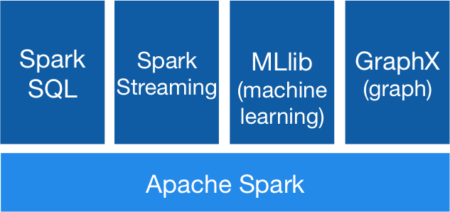
\includegraphics[scale=0.6]{images/spark.png}
  \caption[Spark Besonderheit (01.04.2020)]{Spark Besonderheit (01.04.2020)}
  \url{https://data-science-blog.com/wp-content/uploads/2016/08/spark-stack-1-1-450x212.png}
  \label{fig:Spark_Besonderheit} 
\end{figure}
Mit Spark können eingehende Daten transformiert, fusioniert und auch mathematisch analysiert werden. Typische Anwendungsszenarien von Spark sind interaktive Datenabfragen aus verteilten Datenbeständen und die Verarbeitung von fließenden Daten von Sensoren oder aus dem Finanzbereich oder auch andere. Die Stärke von Spark ist jedoch, dass Machine Learning eingebunden werden kann. Mit Zusätzen wie der Machine Learning Bibliothek (MLiB) oder SparkR (R Bibliotheken die direkt unter Spark verwendet werden). Im Unterschied zu Hadoop, das MapReduce Algorithmen benutzt, kann Spark sehr gut iterative Schleifen verarbeiten. Dies ist sehr wichtig für Machine Learning Algorithmen wie dem K Nearest Neighbour Algorithmus.\\

Seit der Entwicklung von Spark war es darauf ausgelegt, Daten dynamisch im RAM des Server Clusters zu halten und dort zu verarbeiten. Diese In Memory Technologien ermöglichen es besonders schnelle Auswertungen von Daten durchzuführen. Andere Datenbanken wie Redis oder SAP Hana arbeiten In Memory, doch kombiniert Spark diese Technik sehr gut mit der Parallelisierung von Arbeitsschritten über ein Cluster und setzt sich deutlich von anderen Datenbanken ab. Im Feld von Big Data werden aus Kostengründen noch oft mechanisch arbeitende Magnet Festplatten eingesetzt. Doch selbst mit zunehmender Verbreitung von sehr viel schnelleren SSD Festplatten, ist der Arbeitsspeicher hinsichtlich der Zeiten für Zugriff und Schreibbefehle von Daten unschlagbar. Einige Unternehmen berichten von einem hohen Geschwindigkeitsvorteil zu Hadoop.\\

Doch kann Spark nicht nur im Tera-, sondern auch im Petabyte Bereich analysieren. Große Cluster können aus tausenden physikalischen oder virtuellen Server bestehen und auch von Spark eingesetzt werden. Auch ist Spark ein echtes Big Data Framework. Ein Cluster skaliert mit seiner Größe linear in seiner Leistungsfähigkeit. Apache Spark bringt zudem auch sehr viele Bibliotheken und APIs mit, die mit den Programmiersprachen Java, Python, R und Scalar angesprochen werden können.\\

Diese sind ohne Zweifel die verbreitetsten Sprachen, wenn es um Data Science geht. Durch die Flexibilität und geringe Rüstzeit wird Spark in vielen Projekten eingesetzt. Zudem kann es eine große Herausforderung sein ein Data Science Team mit gleichen Programmiersprachen Skills aufzubauen. Durch die Nutzung mehrerer Programmiersprachen kann Spark dieses Problem teilweiße lösen, beziehungsweise kann es so umgangen werden. Durch die APIs, die Spark zur Verfügung stellt können auch Daten von vielen verschiedenen Systemen abgegriffen werden. Beispiele wären hier Cassandra \ref{ssec:Cassandra} oder MongoDB \ref{ssec:MongoDB}.
\subsubsection{Gängige Anwendungsbeispiele für Spark}
\paragraph{ETL Datenintegration}\mbox{} \\
Spark eignet sich sehr gut um Daten aus unterschiedlichsten Quellen zu filtern und diese zu bereinigen um sie letztendlich zusammenzuführen. 
\paragraph{Interaktive Analysen}\mbox{} \\
Außerdem eignet sich Spark aufgrund seines Abfrage Systems fantastisch um interaktive Analysen von großen Datenmengen durchzuführen. Es gibt typische Fragestellungen die aus dem Buisness Analytics kommen. Diese können beispielsweise lauten, welche Quartalszahl für bestimmte Vertriebsregionen vorliegt, oder wie hoch die Produktionskapazitäten sind. Hier muss der Data Analyst nur die richtige Frage stellen und Spark liefert die richtige Antwort. 
\paragraph{Echtzeit Analysen von Datenströmen}\mbox{} \\
Mit Spark werden heute noch Massen von Maschinen- beziehungsweise Finanzdaten im Sekundentakt ausgewertet. Für Spark ist dies ein gängiges Einsatzgebiet. Daten, die von vielen verschiedenen Systemen generiert werden, können mit Spark ohne Probleme in einer hohen Geschwindigkeit zusammengeführt und sogleich analysiert werden. Ein Beispiel aus der Finanzwelt wäre, dass Kredikarten Unternehmen Spark dazu benutzen um in naher Echtzeit auf potenzielle Kreditkartenmissbräuche zu bemerken. 
\paragraph{Machine Learning}\mbox{} \\
Durch die Fähigkeiten die Spark hat wird es oft von vielen als erste Wahl zu Machine Learning empfohlen. Dies ist der Fall, da Spark Daten iterativ im Speicher und parallel in einem Cluster durchlaufen kann.

\subsection{Python [AA]}
\begin{figure}[H]
\centering
  
\includegraphics[scale=0.75]{images/python.png}
  \caption[Python (01.04.2020)]{Python (01.04.2020)}
  \url{https://i.pinimg.com/originals/0f/60/19/0f6019e15f1d8ae07e7e8ea16d242676.png}
  \label{fig:Python}
\end{figure}
Folgendes Kapitel wurde mit der folgenden Quelle bewerkstelligt. (vgl. \cite{bigdata_python_2020})
\subsubsection{Allgemein}
„Python ist eine Programmiersprache, die dank ihrer klaren Syntax und einfachen Lesbarkeit leicht zu erlernen ist und sich sehr vielseitig einsetzen lässt. Für die gängigen Betriebssysteme ist Python frei verfügbar. Die üblichen Programmierparadigmen wie die objektorientierte oder funktionale Programmierung werden unterstützt.“~\cite{bigdata_python_2020}
\subsubsection{Zentrales Merkmal von Python}
Der Ruf von Python ist ein guter, da es eine einfache und saubere Programmiersprache ist die eine klare Struktur hat. Der Programmcode ist intuitiv benutzbar und gleichzeitig leicht lesbar. Obwohl Python einfach ist, kann es gut skalieren und ist auch für komplexe Softwareprojekte einsetzbar. Damit Python so einfach und übersichtlich ist, kommt es mit sehr wenigen Schlüsselwörter aus. Außerdem verwendet Python dazu Einrückungen als Strukturierungselemente.\\

Im Gegensatz zu anderen Sprachen sind verschiedene Programm Blöcke nicht durch bestimmte Schlüsselwörter oder Klammern markiert, sondern durch einfache Einrückungen im Code. Ein weiteres Merkmal von Python ist die automatische Speicherverwaltung. Durch die dynamische Typisierung ist es nicht notwendig, Typen von Variablen oder Funktionsargumente im Vorhinein zu definieren.\\

Ein weiterer Punkt ist, dass niemand in Python an einen bestimmten Programmierstil gebunden ist. So kann für jede Aufgabe der optimale Programmierstil gewählt werden. Zusätzlich ist es möglich verschiedenste Python Programme in andere Sprachen einzubetten.
\subsubsection{Vorteile von Python}
Python bietet eine Vielzahl von Vorteilen. Zum Beispiel ist ein großer Vorteil von Python, dass es durch die einfache Syntax eine einfach zu lernende Sprache ist. Der größte Vorteil ist, dass Python eine schnelle Programmiersprache ist die viele Data Analystinnen und Analysten oder Machine Learning Prozesse benutzen. Deswegen wird Python oft für den ETL Prozess oder für die Analyse verschiedenster Daten benutzt. Python ist außerdem eine Objektorientierte Sprache, die komplexe Datenstrukturen verwalten und verarbeiten kann. Die Flexibilität von Python ist ein Grund warum die Programmiersprache von Data Analystinnen und Analysten gemocht wird. Durch diese Vorteile ist es klar, dass Python oft für Data Analytics benutzt wird.
\subsubsection{Philosophie von Python}
Hier sind alle Grundsätze von Python aufgelistet. Die „Zen of Python":\\
„Beautiful is better than ugly. \\
Explicit is better than implicit. \\
Simple is better than complex. \\
Complex is better than complicated. \\
Flat is better than nested. \\
Sparse is better than dense. \\
Readability counts. \\
Special cases aren't special enough to break the rules. \\
Although practicality beats purity. \\
Errors should never pass silently. \\
Unless explicitly silenced. \\
In the face of ambiguity, refuse the temptation to guess. \\
There should be one-- and preferably only one --obvious way to do it. \\
Although that way may not be obvious at first unless you're Dutch. \\
Now is better than never. \\
Although never is often better than *right* now. \\
If the implementation is hard to explain, it's a bad idea. \\
If the implementation is easy to explain, it may be a good idea. \\
Namespaces are one honking great idea -- let's do more of those!" \cite{python_pep_2020}
\subsection{Pyspark [AA]}
\begin{figure}[H]
\centering
  
\includegraphics[scale=0.7]{images/pyspark.png}
  \caption[Pyspark (01.04.2020)]{Pyspark (01.04.2020)}
  \url{https://i.pinimg.com/originals/97/e2/e1/97e2e161dafc63a9e98e5f350425ba39.png}
  \label{fig:Pyspark}
\end{figure}
Informationen wurden von der folgenden Quelle übernommen und überarbeitet. (vgl. \cite{says_pyspark_2020})
\subsubsection{Allgemein}
PySpark ist eine Python API die es ermöglicht Spark und Python zu verbinden. Diese Erweiterung wurde von der Apache Spark Community entwickelt und veröffentlich um Python in Spark zu benutzen. Wenn PySpark benutzt wird, kann leicht mit Resilient Distributed Databases gearbeitet und diese integriert werden. Außerdem gibt es eine Anzahl von Funktionen die Pyspark gut mit großen Datensätzen arbeiten lässt. Sei es eine Funktion auf die Daten auszuführen oder diese zu analysieren.
\subsubsection{Hauptfunktionen von Pyspark}
\begin{itemize}
\item{Real time computations} \mbox{} \\
Da Pyspark auf In Memory Technologien zurückgreift, zeigt sich eine geringe Latenzzeit.
\item{Polyglot} \mbox{} \\
Pyspark kann auch mit anderen Sprachen wie Scala, Java, Python oder R benutzt werden. Dadurch ist es ein oft genutztes Framework das verwendet wird um große Datenmengen zu analysieren.
\item{Caching and Disk Persistence} \mbox{} \\
Es bietet ein gutes Caching und eine gute Persistenz der Daten.
\item{Fast processing} \mbox{} \\
Ein weiterer Vorteil ist, dass PySpark um einiges schneller ist als andere Frameworks die mit Big Data arbeiten. 
\item{Works well with RDDs} \mbox{} \\
Da Python dynamisch ist, hat es den Vorteil, wenn es mit RDDs arbeitet.
\end{itemize}
\subsubsection{Nutzen von Pyspark}
Python ist eine verbreitete Sprache bei Data Scientists und Data Analystinnen und Analysten. Auf der anderen Hand ist Spark ein starkes Tool um mit Big Data umzugehen. Deswegen hat die Spark Community, PySpark entwickelt um beide zu verbinden.




\subsection{Docker [FK]}
\begin{figure}[H]
    \centering
    
\includegraphics[scale=.67]{images/DockerLogo.png}
    \caption{Docker (01.04.2020)}
    \url{https://www.netways.de/wp-content/uploads/2016/02/DockerLogo.png}
\end{figure}
Docker ist eine Open-Source Plattform für das Ausliefern von Softwareprodukten. Mit Docker kann man die verschiedenen Teile eines Softwareproduktes wie Datenbanken, Server und Clients in einzelne Umgebungen verteilen, sogenannte Container [\ref{ssec:DockerContainer}]. Somit kann jede Komponente einzeln gestartet, konfiguriert, überwacht und getestet werden. Durch diese Modularität können Container fast unabhängig vom Betriebssystem arbeiten. (vgl. \cite{DockerIntro})
\subsubsection{Container} \label{ssec:DockerContainer}
\begin{figure}[H]
    \centering
    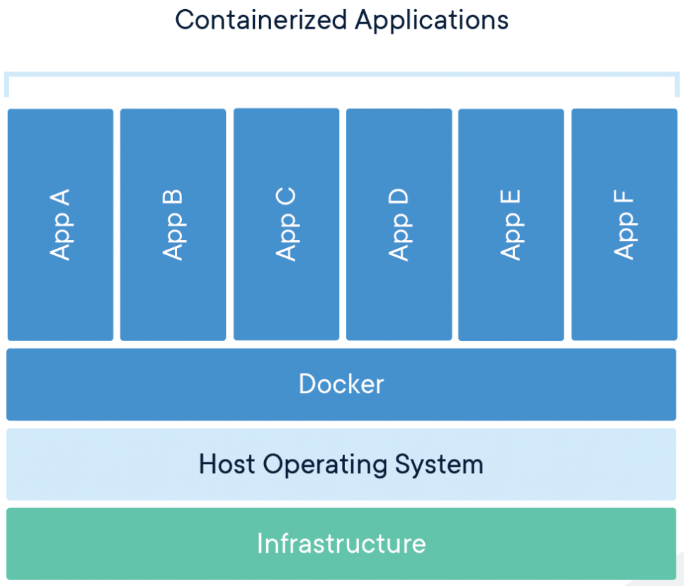
\includegraphics{images/what-is-a-container.png}
    \caption{Docker Container Architektur (01.04.2020)}
    \url{https://www.docker.com/sites/default/files/d8/styles/large/public/2018-11/container-what-is-container.png?itok=vle7kjDj}
    \label{img:what-is-a-container}
\end{figure}

Ein Container ist wie bereits in der Einleitung beschrieben ein abgeschlossenes Objekt welches mit einem oder mehreren Images (\ref{ssec:DockerImages}) als Bauplan erzeugt wird und alle nötigen Dinge beinhaltet was die Software zum Laufen braucht wie die Runtime, Libraries, Einstellungen und natürlich der Code der Applikation. Wie in der Grafik (\ref {img:what-is-a-container}) beschrieben liegen die einzelnen Container auf der Docker Engine auf welche die Container verwaltet und die nötigen Ressourcen vom Betriebssystem zu Verfügung stellt. Dadurch wird sichergestellt das der Code so isoliert von der Umgebung ist wie möglich. (vgl. \cite{DockerContainer})
\subsubsection{Images} \label{ssec:DockerImages}
Ein Docker Image besteht aus mehreren Schichten welche zur Ausführung von Code in einem Docker-Container verwendet wird. Ein Image wird im Wesentlichen aus den Anweisungen für eine vollständige und ausführbare Version einer Anwendung erstellt, die sich auf dem Kernel des Host-Betriebssystems stützt. (vgl. \cite{DockerImage})
Images sind extrem leichtgewichtig, weil sie auf das notwendigste reduziert sind und sicher da diese standardmäßig nicht von anderen Containern beeinflusst werden können. Ein gutes Beispiel dafür ist das Alpine Linux siehe Abbildung (\ref{img:docker-image-size}). Um dennoch mit anderen Containern und anderen Dingen wie dem File System interagieren zu können gibt es sogenannte Networks (\ref{ssec:DockerNetworks}).
\begin{figure}[H]
    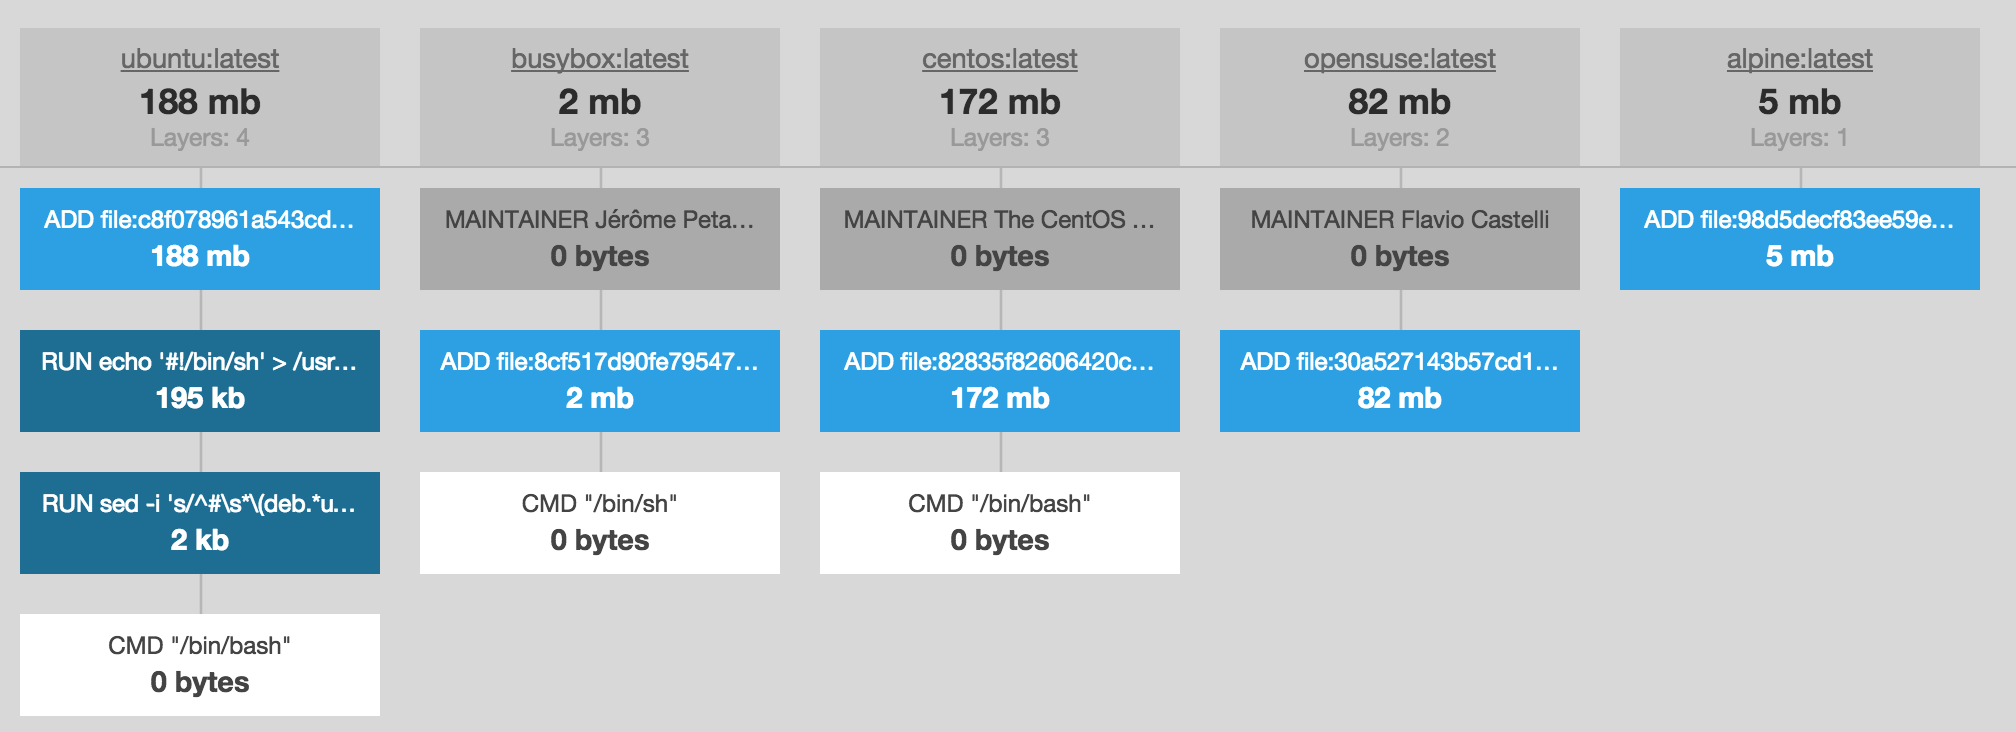
\includegraphics[scale=.40]{images/Docker_Image_Size.png}
    \caption{Docker Image größenvergleich (01.04.2020)}
    \url{https://brianchristner.io/content/images/2015/07/Docker_Image_Size.png}
    \label{img:docker-image-size}
\end{figure}
\subsubsection{Networks} \label{ssec:DockerNetworks}
Networks(Netzwerke) verbinden die einzelnen Container miteinander. Es ist außerdem egal ob die Docker-Hosts unter Windows, Linux oder einer Mischung von beiden laufen. Die Networks verbinden beides Plattform unabhängig.Networks besitzen auch Möglichkeiten Docker unabhängige Systeme zu beeinflussen. Die verschiedenen Network Einstellungen werden im Kapitel Dockerfile [\ref{ssec:Dockerfile}] noch genauer Beleuchtet. (vgl. \cite{DockerNetworks})
\paragraph{Docker Produkte:}\mbox{}\\
\begin{itemize}
    \item Docker Toolbox [\ref{ssec:DockerToolbox}]
    \item Docker CE [Community Edition) (\ref{ssec:DockerCE}]
    \item Docker EE [Enterprise Edition) (\ref{ssec:DockerEE}]
    \item Docker Hub [\ref{ssec:DockerHub}]
    \item Docker Desktop [\ref{ssec:DockerDesktop}]
    \item Orchestration anhand von Kubernetes (\ref{ssec:DockerOrchestration}]
    \item Dockerfile [\ref{ssec:Dockerfile}]
    \item Docker-compose [\ref{ssec:Docker-Compose}]
\end{itemize}
\subsubsection{Docker Toolbox} \label{ssec:DockerToolbox}
Docker Toolbox ist eine veraltete Version von Docker. Es ist dennoch wichtig, weil ältere Betriebssysteme (Bsp. Windows 8) dennoch Docker installieren und verwenden können. Jedoch geht der große Vorteil von Docker verloren, weil anstatt der Docker Engine alles auf einer VirtualBox aufbaut. Somit geht einiges an Performance verloren, was aber beim Entwickeln kein Hindernis darstellt. Ein weiterer Use-Case der Docker Toolbox ist das verwenden auf PCs mit Windows 10 Home denn in der Home Version wird Hyper-V [\ref{Hyper-V}] nicht unterstützt. (vgl. \cite{DockerToolbox})
\subsubsection{Docker CE (Community Edition) / Docker Engine}\label{ssec:DockerCE}
Docker Community ist die klassische Open Source Version von Docker. Früher genannt Docker Engine. Alle oben genannten Funktionen sind ganz normal vorhanden ohne Kürzungen oder Ähnliches. Der geschriebene Sourcecode ist ebenfalls derselbe wie bei der Enterprise-Edition, weil beides auf dem Open Source Code von Docker aufbauen. Es gibt eine Stabile und eine experimentelle Version, bei welcher die neuesten Funktionen vorhanden sind, es aber noch immer Sicherheitslücken und Fehler geben kann. Vierteljährlich kommt eine neue Stabile Version heraus und jeden Monat gibt es eine neue experimentelle Version. (vgl. \cite{DockerCE})
\subsubsection{Docker EE (Enterprise Edition)}\label{ssec:DockerEE}
Docker Enterprise ist dafür da das Unternehmen ihre Container einfacher verwalten, starten und sichern können. Dabei gibt es drei verschiedene Versionen: Basic, Standard und Advanced.
\begin{itemize}
    \item Basic
    \begin{itemize}
        \item Spezielle Enterprise Betriebssysteme wie Windows Server oder Red Hat Enterprise Linux können verwendet werden.
        \item „same day“ Docker Support.
        \item Zertifizierte Container und Plugins aus dem Docker Hub.
    \end{itemize}
    \item Standard (Aufbauend auf Basic)
    \begin{itemize}
        \item Erweiterte Container- und Imageverwaltung.
        \item LDAP/AD Benutzer Integration. (\ref{sec:AD})
        \item Rollen basierte Zugriffskontrolle.
    \end{itemize}
    \item Advanced (Aufbauend auf Standard).
    \begin{itemize}
        \item Docker Security Scanning überprüft ob Images und Container frei von bekannten Sicherheitslücken sind.
        \item Kontinuierliche Überwachung von Schwachstellen.
    \end{itemize}
\end{itemize}
Wie bereits bei Docker Community angesprochen gibt es keine Unterschiede in der Funktionsweise der Docker Engine. Was jedoch auch bedeutet das man für seine 750\$ pro Prozessor pro Jahr für die Basic, 1500\$ für die Standard oder 2000\$ für die Advanced Version für Linux(Windows ist billiger) kein besseres Produkt bekommt, sondern nur oben genannte Boni. (vgl. \cite{DockerEE}, \cite{DockerEELicensing}, \cite{DockerEEPricing})
\subsubsection{Docker Hub} \label{ssec:DockerHub}
Docker Hub ist eine Website zur Verfügung gestellt von Docker wo User auf der ganzen Welt ihre Container Images hochladen können und sie somit mit anderen Usern teilen können. Man muss dabei nicht immer auf fragwürdige Quellen vertrauen, denn es gibt sogenannte „Official Images“ welche von Docker selbst veröffentlicht wurden und außerdem verifizierte und zertifizierte Veröffentlicher um auf der sicheren Seite zu sein das keine Malware im Image steckt. Das Container Image rauf- und runterladen ist dabei meistens gratis, jedoch muss man für die Erstellung von mehr als einem privaten Repository einer monatlichen Zahlung zustimmen. (vgl. \cite{DockerHub})
\subsubsection{Docker Desktop}\label{ssec:DockerDesktop}
Docker Desktop ist, wer hätte es gedacht, eine Desktop App für Windows und Mac OS. Der Download von Docker Desktop lädt automatisch alle benötigten Dateien, um die Community Version von Docker zu verwenden. Leider bedeutet das auch das Nutzer mit Windows 10 Home oder niedrigere Versionen von Windows dieses Tool nicht verwenden können und sich mit der CLI-Only (Command Line Interface Only) Version der Docker Toolbox zufriedengeben müssen. Sollte man aber Windows 10 Pro oder Enterprise besitzen, hat man mit Docker Desktop die Möglichkeit im Dashboard alle laufenden Container inklusive Kubernetes zu verwalten. Mit einem einzigen Klick kann man den Container somit kinderleicht Starten, Stoppen, Neustarten, den Port ändern oder direkt per Command Line darauf zugreifen. Außerdem kann man die Logs, die Image Einstellungen und diverse Statistiken betrachten. (vgl. \cite{DockerDesktopDashboard}, \cite{DockerDesktop}) 
\begin{figure}[H]
    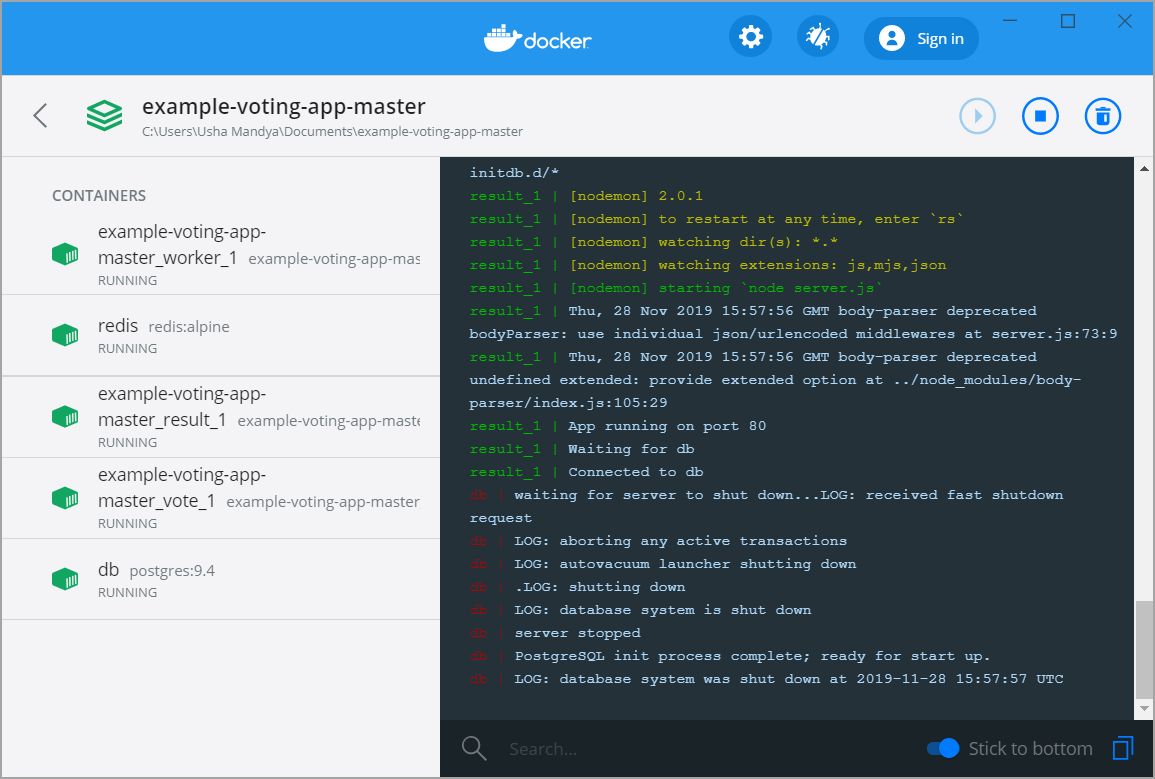
\includegraphics[scale=.65]{images/docker-desktop-view1.png}
    \caption{Docker Desktop Dashboard mit CLI (01.04.2020)}
    \url{https://docs.docker.com/docker-for-windows/images/application-view.png}
    \label{img:docker-desktop-view1}
\end{figure}
\begin{figure}[H]
    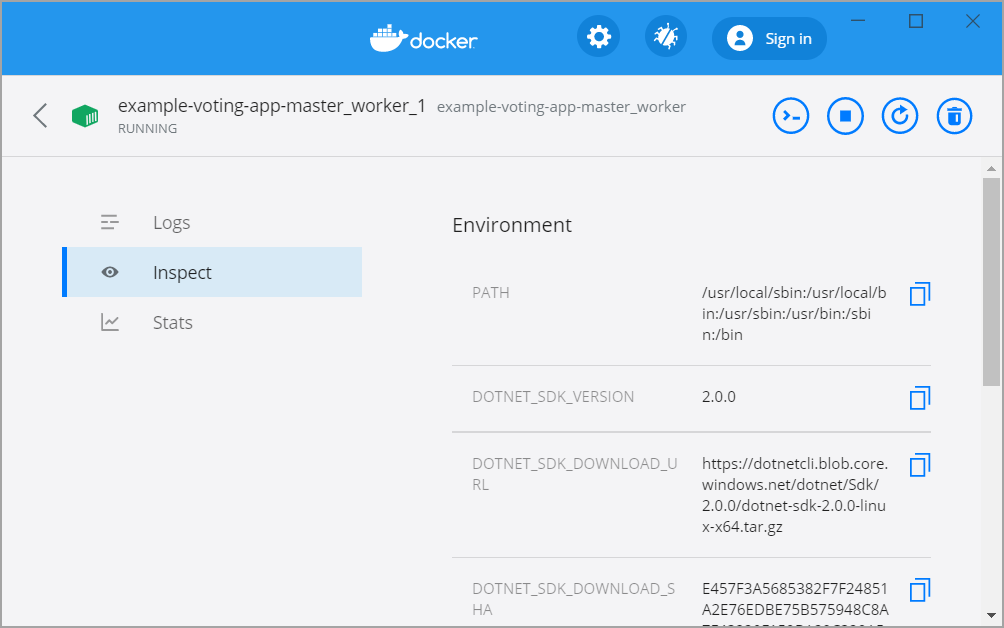
\includegraphics[scale=.70]{images/docker-desktop-view2.png}
    \caption{Docker Desktop Dashboard mit Monitoring (01.04.2020)}
    \url{https://docs.docker.com/docker-for-windows/images/container-view.png}
    \label{img:docker-desktop-view2}
\end{figure}
\subsubsection{Orchestration (with Kubernetes)}\label{ssec:DockerOrchestration}
\begin{figure}[H]
    \includegraphics[scale=.50]{images/kubernetesLogo.png}
    \caption{Docker mit Kubernetes (01.04.2020)}
    \url{https://miro.medium.com/max/787/1*y320p_dXJmr5PMGRiXioyw.png}
\end{figure}
\paragraph{Was ist Orchestration und wofür wird sie benötigt}\mbox{}\\
Von Orchestration ist die Rede, wenn automatisiert viele verschiedene Computer zusammenarbeiten, um eine möglichst hohe Leistung und/oder hohe Verfügbarkeit zu erzeugen. Durch diese vielen verschiedenen Systeme und Programme steigt der Aufwand exponentiell mit der Anzahl der sogenannten Knotenpunkte(nodes). Dieser Aufwand kann eigenhändig ab einem gewissen Punkt nicht mehr bewältigt werden. Die Lösung: Automatisierung. Der Feine unterschied zwischen Automatisierung und Orchestrierung ist das die Orchestrierung auf der Automatisierung aufbaut. Eine einzelne Aufgabe kann Automatisiert werden aber wenn viele automatisierte Aufgaben zusammengeschlossen werden nennt man die Orchestrierung. 
\paragraph{Kubernetes und Docker}\mbox{}\\
Kubernetes wurde von Google entwickelt und 2014 als Open Source veröffentlicht. Kubernetes ermöglicht viele verschiedene Container zu verbinden, ohne dass man sich ständig Gedanken machen muss wie die Container untereinander kommunizieren, in welcher Reihenfolge die Container gestartet werden müssen oder was bei Programmabstürzen passiert. (vgl. \cite{DockerOrchestration})
\paragraph{Vorteile von Kubernetes}\mbox{}\\
\begin{itemize}
	\item Sollte ein Container abstürzen oder die Maschine defekt sein kann ein neuer Container auf einer anderen Maschine automatisch gestartet werden.
	\item Die Belastung der Container wird auf verschiedene Maschinen aufgeteilt.
	\item Es können verschiedene Instanzen eines Containers existieren wie z.b. bei einer Datenbank. Somit können kosten für die Anschaffung von extrem viel Speicher auf einer Maschine gespart werden.
	\item Wenn sich die Auslastung eines Containers verändert können Instanzen hinzugefügt oder weggegeben werden.
	\item Derselbe Code kann auf mehreren Maschinen gleichzeitig laufen
\end{itemize}
(vgl. \cite{DockerKubernetes})
\subsubsection{Das Dockerfile}\label{ssec:Dockerfile}
Das Dockerfile enthält die Logik, um ein Image aufzubauen. Das Dockerfile ist ein Text Dokument, welches die ganzen Kommandos enthält, die auch ein User auf der CMD [\ref{sec:CMD}] selber ausführen könnte. Der große Vorteil dabei ist das mit einem einzigen „docker build“ alle Kommandos automatisch ausgeführt werden. (vgl. \cite{Dockerfile})
\begin{figure}[H]
    \includegraphics{images/dockerfile_example.PNG}
    \caption{Allgemeines Dockerfile Beispiel}
    \label{img:dockerfile_example}
\end{figure}
So könnte ein gesamtes Dockerfile aussehen.
Nun werden die einzelnen Teile erklärt:
\paragraph{Das FROM statement}\mbox{}\\
Mit dem FROM Statement kann ein bereits existierendes Image verwendet werden und auf dessen Basis weitergearbeitet werden. In diesem Fall wird das FROM genutzt, um eine dotnet core 3.0 sdk (Eine C\# Applikation) mit allem was es benötigt zu verwenden. Sollten mehrere FROM Statements in einem Dockerfile sein teilt FROM in mehrere Umgebungen. Nachdem in unserem Beispiel später noch ein FROM Statement steht, müssen wir das erste FROM Statement mit „AS build“ benennen, um es in dem COPY Befehl am Schluss wiederverwenden zu können. 
\paragraph{Das RUN Statement}\mbox{}\\
Mit dem RUN Statement können Befehle wie in der Command Line ausgeführt werden. Hier werden noch einige Linux Funktionen nach installiert. Allgemein kann aber alles Mögliche ausgeführt werden
\paragraph{Das WORKDIR Statement}\mbox{}\\
Das WORKDIR Statement setzt einfach das Verzeichnis zu dem eingegebenen. Wenn das Verzeichnis nicht existiert wird es erstellt.
\paragraph{Das COPY Statement}\mbox{}\\
Das COPY Statement kopiert einfach die Files von einem Ort zum anderen. Äquivalent zu „RUN cp …“
\paragraph{Das EXPOSE Statement}\mbox{}\\
Das EXPOSE Statement öffnet den Port der als Parameter mitgegeben wird. Beachte: der Port wird nur in dem Container geöffnet
\paragraph{Das ENTRYPOINT Statement}\mbox{}\\
Das ENTRYPOINT Statement fungiert als ein Aufruf eines Kommandos. Der erste Parameter zeigt das Kommando, das ausgeführt werden soll und danach können so viele Parameter folgen wie man braucht. In diesem Beispiel wird der Befehl "dotnet" aufgerufen und als Parameter bekommt der Befehl "Testprogramm.dll" mit
\subsubsection{Das Docker-Compose}\label{ssec:Docker-Compose}
Das Docker-Compose ist ein File in welchem mehrere Docker Container in der gewünschten Reihenfolge und Parametern automatisch aufgerufen werden können. Somit muss man nicht jeden Container und jedes Netzwerk einzeln per Hand aufrufen, sondern muss nur den Befehl: „docker-compose up“ ausführen und man hat sofort alle Container gestartet. Dadurch verringert sich nicht nur der Aufwand enorm, sondern auch die Fehler Quote, wenn man z.B. die Container nicht in der richtigen Reihenfolge oder mit den falschen Parametern startet.
Ein docker-compose kann entweder ein .yml oder .yaml File sein. Es ist jedoch immer wichtig die Einrückungen richtig zu setzen, weil es keine geschwungenen Klammern oder Ähnliches gibt wie in anderen Programmiersprachen. Allgemein ist es ähnlich zu dem oben genannten Dockerfile, weil wieder mit Statements beschrieben wird, was gemacht werden soll. 
\begin{figure}[H]
    \includegraphics{images/docker-compose_example.PNG}
    \caption{Einfaches docker-compose Beispiel}
    \label{img:docker-compose_example}
\end{figure}
\subsubsection{Das Version Statement}
Das allererste in einem docker-compose ist das Version Statement. Damit wird dem Interpreter gesagt in welcher Version das folgende File geschrieben ist.
\subsubsection{Das Services Statement}
Das Services Statement beinhaltet alle Container, die gestartet werden sollen. Jedes Service bekommt einen Namen und den Pfad, wo das zugehörige Dockerfile liegt. Existiert bereits online ein fertiges Image, kann darauf verwiesen werden. Mit „ports“ kann man die offenen Ports festlegen. Rechts vom Doppelpunkt steht dabei der geöffnete TCP Port im Container und dieser wird auf den Docker Host Links vom Doppelpunkt gemapped. Bsp.: 8080:80 wenn man nun auf Port 8080 des Servers zugreift wird auf den Container am Port 80 weitergeleitet. Im nächsten Schritt wird festgelegt welche Services zuerst gestartet werden sollen. Im Bereich "volumes" kann eine Schnittstelle zu dem Host System geöffnet werden, um Daten permanent zu speichern welche sonst durch das neu erstellen des Containers verloren gehen würden. Mit dem Networks Bereich kann das Netzwerk ausgewählt werden, zu welchem das jeweilige Service gehört.
\subsubsection{Das Networks Statement}
Mit dem Networks Statement können ein oder mehrere Netzwerke erstellt werden. Wenn man das Netzwerk als extern deklariert kann man auf ein bereits existierendes Netzwerk von z.b. einem anderen docker-compose zugreifen. Außerdem kann man dem Netzwerk einen eigenen IP Adressraum geben. Das Networks Statement wird immer vor den Services aufgerufen.



\subsection{REST API [FK]} \label{sec:REST} 
Anmerkung: Folgendes wurde auf Basis von diesen Quellen geschrieben: (vgl. \cite{RestApi}, \cite{RestKonzept})
Rest bedeutet Representational State Transfer. API bedeutet Application Programming Interface.
Rest ist eine Möglichkeit über das Internet Daten zwischen verteilten Systemen auszutauschen. Es ist aber weder ein neues Protokoll noch Standard, sondern zeichnet jene Verfahren aus welche über das http Protokoll Daten versenden. Die versendeten Daten müssen aber nicht ein http Dokument sein denn das würde viel zu viele Stylings mitsenden, welche ungenutzt wären. Statt http wird JSON [\ref{sec:json}] oder XML [\ref{sec:xml}] verwendet. Diese beiden Formate können ausschließlich die Rohdaten enthalten und sind somit optimal. 
\begin{figure}[H]
    \includegraphics[scale=.9]{images/Rest-API.png}
    \caption{Rest Darstellung (01.04.2020)}
    \url{https://www.seobility.net/de/wiki/images/f/f1/Rest-API.png}
    \label{img:Rest}
\end{figure}
Wie bereits auf der Grafik zu sehen gibt es Grundsätzlich 4 verschiedene REST Requests. 
\subsubsection{GET Requests}
Mit dem GET Schlüsselwort wird dem empfangenen Server angezeigt das der Sender Daten haben will. Als Rückgabewert gibt es einen Return Code der bei Erfolg 200 (OK) lautet und bei Fehlschlag entweder 404 (Not Found) oder 400 (Bad Request). Außerdem wird bei Erfolg ein Body mit den Daten als JSON oder XML zurückgegeben.
Ein Typischer GET Request in cURL auf der Konsole würde so aussehen:
\begin{lstlisting}
    curl https://popularsite.com/getAllItems
\end{lstlisting}
\subsubsection{POST Requests}
Mit dem POST Request können Daten welche im Empfänger noch nicht existieren versendet werden. Bei Erfolg wird 201 (Created) zurückgegeben.
\subsubsection{PUT Requests}
Mit dem PUT Request können auch Daten erstellt werden aber hauptsächlich wird er dafür verwendet bestehende Datensätze zu Updaten. Wenn man sich aber nicht sicher ist ob der Datensatz (zum Beispiel ein Kunde) bereits existiert kann PUT verwendet werden um den Kunden neu hinzuzufügen sollte er noch nicht existieren ansonsten wird der Bestehende bearbeitet.
\subsubsection{DELETE Requests}
Mit dem DELETE Request können Daten auf dem Server gelöscht werden. 
\subsection{Die Architekturprinzipien von REST}
\subsubsection{Zustandslosigkeit}
Alle REST anfragen arbeiten „stateless“. Das bedeutet das in jedem Request alle Infos enthalten sein müssen damit der Empfänger genau weiß was zu tun ist. Nach jedem Request hat der Empfänger keine Informationen mehr wer ihm daten Geschickt hat oder woher. Somit erhöht sich die Skalierbarkeit und die Zuverlässigkeit, weil der Server nicht ständig eine Verbindung halten muss wie zum Beispiel bei einer Websocket Verbindung. Der Nachteil ist dabei eine Höhere Netzwerkauslastung 
\subsubsection{Caching}
Clients können die Antworten vom Server speichern umso die Netzwerkauslastung zu reduzieren. Der Nachteil dabei ist jedoch auf veraltete Daten zuzugreifen.
\subsubsection{Client-Server Modell}
Um Server besser Skalieren zu lassen muss der Client vom Server getrennt sein. Dies hat außerdem den Vorteil das der Client auf verschiedenen Plattformen ausführbar ist.
\subsubsection{Gleichartige Schnittstellen}
Alle REST Services nutzen das gleiche entkoppelte Interface. Somit wird sichergestellt das alles so einfach und einheitlich wie möglich ist. Der Nachteil dabei ist das nicht auf spezielle Anforderungen eingegangen werden kann.
\subsubsection{Hierarchisches System}
REST ist in mehreren Schichten aufgebaut wie folgende Grafik zeigt [\ref{img:Rest_Schichtenmodell}]. Jede Schicht kann aber nur die Anliegende „sehen“. 
\begin{figure}[H]
    \centering
    \includegraphics[scale=1]{images/REST_schichtenmodell.jpg}
    \caption{Rest Schichtenmodell (01.04.2020)}
    \url{https://images.vogel.de/vogelonline/bdb/1220900/1220968/4.jpg}
    \label{img:Rest_Schichtenmodell}
\end{figure}

\subsection{Elasticsearch [FK]}\label{sec:ES}

\begin{figure}[H]
    \centering
    \includegraphics[scale=1]{images/ESLogo.PNG}
    \caption{Elasticsearch (01.04.2020)}
    \url{https://www.tudock.de/fileadmin/blog/blog_beitragsbilder/2018/Elasticsearch_-_Horizontal_Text_-_Full_Color_712.png}
\end{figure}
Elasticsearch ist eine in Java geschriebene Suchmaschine und zugleich NoSQL Datenbank. Es basiert auf der Volltextsuchmaschine Apache Lucene. Es ist eine dokumentenorientierte Datenbank und speichert die Dokumente im JSON [\ref{sec:json} Format. Diese Dokumente werden auch sofort indexiert um möglichst hohe Abfragegeschwindigkeiten zu ermöglichen. Der Suchserver kann als verteiltes System mit mehreren Rechnern betrieben werden und setzt damit auf eine hohe Verfügbarkeit und sehr gute Lastverteilung. „Elasticsearch zerteilt jeden Index [\ref{sec:Index}] in mehrere Stücke, so genannte shards (Scherben, Bruchstücke). Die shards eines Indexes können vom Anwender bei Bedarf auf mehrere Server (nodes) aufgeteilt werden (die Gruppe heißt Cluster), um die Rechenlast zu verteilen oder um Serverausfälle zu kompensieren. Läuft die Suchmaschine auf mehreren nodes, so wird einer als Master node der Gruppe bestimmt.“ \cite{PhysAufbau}
Neben Elasticsearch gibt es auch noch andere „gratis“ Volltextsuchmaschinen wie zum Beispiel der größte Konkurrent Apache Solr. Beide sind im Kern Open-Source Projekte haben aber ganz unterschiedliche Eigenschaften. Kurz die Unterschiede zusammengefasst ist Solr besser, wenn es um statische Daten geht aufgrund seiner Caches und Elasticsearch ist besser bei Logdateien und der Analyse von Daten. Ein detaillierter Vergleich würde hier den Rahmen sprengen, denn es geht ja um Elasticsearch. Wer dennoch einen genauen Vergleich will sollte sich diesen Artikel durchlesen: \cite{ESvsSolr}
\subsection{Abfragesprachen}
Die Standardabfragesprache von Elasticsearch ist „Query DSL“ (Domain Specific Language) welche auf JSON basiert um Abfragen durchzuführen. Elasticsearch bietet aber auch noch eine weitere Abfragesprache um es auch SQL gewöhnten Programmierern recht zu machen nämlich Elasticsearch SQL.
\subsection{Query DSL}
Grundsätzlich gibt es zwei verschiedene Abfragesprachen: „Leaf query clauses“ und „Compound query clauses“.
Bei Leaf queries wird nach einem bestimmten Wert in einem Feld gesucht.


Bei Compound query clauses werden Leaf und Compound abfragen so verpackt damit mehrere Abfragen auf logische Weise kombiniert werden können.
(vgl. \cite{ESQueryDsl}) 
\subsubsection{Relevance Score}
Die Relevanz Punktzahl gibt an wie wahrscheinlich jedes einzelne Dokument dem entspricht, was die Abfrage fordert. Die Zahl wird in jedem Dokument als meta Feld dargestellt ( \_score ). Jeder Abfragetyp bewertet den Score unterschiedlich. Außerdem hängt die Bewertung davon ab, ob die Abfrageklausel in einem Abfrage- oder Filterkontext ausgeführt wird. (vgl. \cite{DSLQueryFilter})
\subsubsection{Abfrage Kontext}
Im Abfrage Kontext wird überprüft wie gut ein Dokument auf die Aktuelle Abfrage zutrifft. Je nachdem wie gut das Dokument passt wird es als passend deklariert und die Relevanz Punktzahl ermittelt. Der Abfrage Kontext wird benutzt, wenn der „query“ Parameter in der Suche befüllt wird. (vgl. \cite{DSLQueryFilter})
\subsubsection{Filter Kontext}
Beim Filter Kontext wird überprüft, ob die Abfrage genau zutrifft. Bsp: Ist das „age“ Feld größer 60.
Es wird dabei keine Punktzahl bestimmt, sondern einfach mit Ja oder Nein bestimmt, ob das Dokument zu der Abfrage passt. Dies funktioniert natürlich am besten mit gut strukturierten Daten, um welche man sich selbst kümmern muss , da es ja eine schemafreie Datenbank ist. Ein weiterer Vorteil neben der klaren Ja/Nein Antwort ist das öfters ausgeführte Abfragen in einem Cache gespeichert werden, was wiederum die Performance stark erhöht.
Genutzt wird der Filter Kontext in Abfragen mit „filter“ oder „must/must\_not“ Parametern. (vgl. \cite{DSLQueryFilter})
\subsubsection{Beispielabfrage}
Folgendes Beispiel zeigt die Verwendung von Abfrage und Filter Kontexte. Dokumente welche folgenden Bedingungen erfüllen würden in der Suche gefunden werden.
\begin{itemize}
    \item Der Titel im Dokument enthält das Wort: „Search“.
    \item Das Inhaltsfeld enthält das Wort: „Elasticsearch“.
    \item Im „status“ feld steht nur „published“.
    \item Das Feld „publish\_date“ enthält ein Datum ab dem 1. Januar 2015.
\end{itemize}
\begin{figure}[H]
    \centering
    \includegraphics[scale=1]{images/ES_queryBsp.PNG}
    \caption{ES Beispielabfrage (01.04.2020)}
    \url{https://www.elastic.co/guide/en/elasticsearch/reference/current/query-filter-context.html}
    \label{img:ESexamplebsp}
\end{figure}
\begin{enumerate}
    \item Der „query“ Parameter zeigt den Kontext für die Abfrage an
    \item Die „bool“ und Die „match“ Klauseln geben an das es sich um einen query Kontext handelt. Somit wird die Relevanzpunktzahl für jeweilige Dokumente berechnet.
    \item Der „filter“ Parameter weist darauf hin, dass es sich um einen Filter Kontext handelt. Dokumente die nicht zu dem Filter passen werden aussortiert aber die Punktzahl vom query Kontext wird dabei nicht beeinflusst.
\end{enumerate}
Neben diesen Abfragen gibt es noch viele mehr aber das würde den Rahmen dieser kurzen Übersicht sprengen. (vgl. \cite{DSLQueryFilter})
\subsection{Elasticsearch SQL}
„Elasticsearch SQL ist eine X-Pack-Komponente, mit der SQL-ähnliche Abfragen in Echtzeit gegen Elasticsearch ausgeführt werden können. Ob über die REST-Schnittstelle, die Befehlszeile oder JDBC [\ref{sec:JDBC}], jeder Client kann SQL verwenden, um Daten innerhalb von Elasticsearch nativ zu suchen und zu aggregieren. Man kann sich Elasticsearch SQL als einen Übersetzer vorstellen, der sowohl SQL als auch Elasticsearch versteht und durch die Nutzung der Elasticsearch-Fähigkeiten das Lesen und Verarbeiten von Daten in Echtzeit und in großem Maßstab erleichtert." \cite{Elasticsearch-SQL}
\subsubsection{Vorteile}
Elasticsearch SQL ist nicht einfach eine Übersetzung in die DSL-Abfragesprache, sondern wurde entwickelt, um direkt auf die benötigten Nodes zugreifen zu können. Durch diese Integrierung ins System ist es auch nicht notwendig externe Hardware oder Libraries zu installieren. Außerdem schränkt Elasticsearch SQL die Suchfähigkeiten nicht ein. Aber der wahrscheinlich beste und offensichtlichste Vorteil ist die Möglichkeit, in einer gewohnten Sprache einfach Abfragen machen zu können ohne sich mit der DSL-Abfragesprache befassen zu müssen.
\subsubsection{Nachteile}
Neben mehreren kleineren Problemen bei größeren Mengen an Daten ist das größte Problem, das man seine gespeicherten Daten strukturiert halten muss oder zumindest sollte, wenn man das meiste aus der Sprache herausholen möchte. Somit wird der Verwaltungsaufwand erhöht.
\subsubsection{ES SQL Beispiel}
Anmerkung: Für dieses Beispiel verwende ich die Developer Konsole von Kibana \ref{ssec:devtools}.
Um Beispieldaten hinzuzufügen verwende ich bulk. Es werden drei Personen erstellt, welche die gleichen Eigenschaften besitzen.
\begin{figure}[H]
    \centering
    \includegraphics[scale=1.3]{images/es_sql_import.PNG}
    \caption{ES Beispiel Datenimport}
    \label{img:es_sql_import}
\end{figure}
Um nun eine Abfrage mit SQL zu machen, schreibt man einen POST Request mit dem Schlüsselwort „\_sql?format=txt“.
Außerdem benötigt man einen „query“ Parameter, in welchem die eigentliche SQL-Abfrage geschrieben ist. 
\begin{figure}[H]
    \centering
    \includegraphics[scale=1.3]{images/es_sql_query.PNG}
    \caption{ES Beispiel Suche}
    \label{img:es_sql_query}
\end{figure}
Bei „format=txt“ wird dabei festgelegt, wie die Ausgabe aussehen soll. Im Falle von „txt“ wird das Ergebnis als Tabelle ausgegeben, wie wenn es direkt aus der Konsole kommen würde. Weitere Möglichkeiten sind: json, csv, yaml und noch mehr.
Nun zu der SQL-Abfrage: Nach dem „FROM“ Statement kommt der Index, in welchem gesucht werden soll. „birth\_date“ ist das Feld, das überprüft werden soll. Man merkt, das es ziemlich genau wie normales SQL agiert.
\begin{figure}[H]
    \centering
    \includegraphics[scale=1.3]{images/es_sql_outputTxt.PNG}
    \caption{ES Beispiel Ergebnis}
    \label{img:es_sql_outputTxt}
\end{figure}
(vgl. \cite{EsSql})
\chapter{Praktische Umsetzung}
\section{Testdatensätze[EK]}
\subsection{Aneignungsphase}
Hier in der Aneignungsphase zu den Testdatensätzen werden die Ansätze erwähnt, welche vor der eigentlichen finalen Prototypenentwicklung aufgekommen sind.
\subsubsection{Eigene Oracle-DB}
Im Rahmen der Einarbeitung wurde zum testen von Databus auf eine eigene lokal laufende  Oracle-DB gesetzt. 
\subsubsection{MIC-Datenbank}
Nachdem eine erfolgreiche Testung des Aufzeichnens von Änderungen auf einer lokalen Oracle-DB geglückt ist, wurde der nächste Schritt angegangen. Dieser sollte Datenveränderungen in einer MIC-Datenbank erkennen und weitergeben. In dieser Phase wurde erkannt, dass Databus durch seine Art Daten entgegenzunehmen ein Problem für die MIC darstellt, wie schon näher beim  in 4.2.1 Databus erläutert wurde. Mit dem Wegfallen von Databus begann somit die eigentliche Entwicklung des Prototyps. Dadurch, dass sich auch die Anforderungen der Firma änderten, war nun ein Generator von Nöten, um die weiteren Module verwirklichen und testen zu können.
\newpage

\subsection{Generator in Python}
\subsubsection{Allgemein}
Der Fake-Apache-Log-Generator dient dazu, die Phase-1-Implementierung des Prototyps mit Daten zu beliefern. Die Phase-1 beschreibt den ersten einfachen Ansatz des Prototyps. Es handelt sich hier um ein kleines Programm, welches vom GitHub Nutzer „kiritbasu“ geschrieben wurde. (vgl.\cite{Fake-Apache-Log-Generator})
\vspace{5mm}\par
Das Programm liefert Fake-Apache-Logs, welche wie folgt aussehen:
\begin{figure}[H]
    \centering
    \includegraphics[scale=0.55]{images/apache-faker.png}
    \caption{Log-Output}
\end{figure}
\subsubsection{Zweck}
Die Überlegung zu diesem Generator war, den kompletten Prozess auf das Einfachste herunterzubrechen, um diesen realisierbar zu machen. Später sollte dieser dann in Phase-2 durch einen komplexeren selbst geschrieben Generator ersetzt werden.

\newpage
\subsection{Generator-Gerald}
\subsubsection{Allgemein}
Der Generator-Gerald ist das Modul, welches das Generieren der Zolldaten, wie in 3.2 Datenquellen erwähnt, implementiert und gehört somit zur Phase-2 des Prototyps. Der Generator ist in Kotlin auf Basis der JVM Plattform geschrieben und kann somit auf jedem System, welches das Java-Runtime-Environment installiert hat, laufen. Als Build-Automation-Tool kommt Gradle zum Einsatz, welches sich um die Ausführung der Unit-Tests und den Build-Prozess kümmert, welcher das ganze Programm und seine Dependencies in eine sogenannte Uber-JAR steckt. Dies sorgt dafür, dass das komplette Programm über eine einzige JAR ausführbar ist.
\vspace{5mm}\par
An erster Stelle der Designüberlegungen stand die Frage, auf Basis welcher Daten die Generierung erfolgen soll. Diese Überlegung wurde angeschnitten, um bei der Nutzung des Generators eine gewisse Variation und Bestimmung der generierten Daten zu ermöglichen. Somit wurden fünf Startparameter für den Generator definiert, welche in Form eines JSON-Strings übergeben werden müssen. Die dazu gehörige Datenklasse für die \textit{GenerationParams} sieht wie folgt aus:
\begin{lstlisting}[caption={GenerationParams}, language=Kotlin]
data class GenerationParams(
    val company: String,
    val plant: String,
    val importCountry: String,
    val periodRangeStart: Int,
    val periodRangeEnd: Int
)
\end{lstlisting}
\vspace{4mm}\par
Auf Basis dieser kann der Generator dann den folgenden Zolldeklarationsdatensatz erstellen.
Bei den generierten Daten gibt es vier Arten: 
\begin{itemize}
  \item \textbf{Parameterdaten}, diese werden beim Start des Programms übergeben und bleiben konstant bei jedem generierten Datensatz, auf diesen können Zufalls- und Zeitdaten basieren.
  \item \textbf{Zufallsdaten}, diese werden komplett zufällig unter speziellen Bedingungen, welche auch von anderen Zufallsdaten abhängen können, generiert.
  \item \textbf{Arraydaten}, über den Index wird ein Element aus einem Array ausgewählt.
  \item \textbf{Zeitdaten}, diese werden immer in Abhängigkeit von anderen Zeitdaten von einander generiert, die Parameterdaten zu Periode schränken dabei den Zeitraum ein, in welcher jene vorkommen dürfen.
\end{itemize}
\subsubsection{Verwendung des Generators}
Zum Start des Generators muss zwingend ein JSON-String mit dem \textit{GenerationParams} als erstes Startargument an das Programm übergeben werden. Hier die Namenserläuterungen:
\begin{itemize}
    \item \textit{company} - zweistelliger Kürzel der empfangenden Firma
    \item \textit{plant} - zweistelliger numerischer Code, welcher das Werk, in welches die Ware geliefert wird, identifiziert.
    \item \textit{importCountry} - Ländercode des Empfängerlandes nach ISO 3166-1 alpha 2
    \item \textit{periodRangeStart} - Zeitangabe des Jahres und Monats im Format YYYYMM, legt das erstmögliche Datum für die Generierung fest.
    \item \textit{periodRangeEnd} - Zeitangabe des Jahres und Monats im Format YYYYMM, legt das letztmögliche Datum für die Generierung fest.
\end{itemize}
Alle Parameter müssen gültig belegt werden, einzige Ausnahme bilden die zwei Parameter \textit{periodRangeStart}  und \textit{periodRangeEnd}. Diese können mit dem Wert 0 belegt werden, welcher dafür sorgt, dass intern \textit{periodRangeStart} auf den ersten Tag des aktuellen Jahres gesetzt wird und \textit{periodRangeEnd} auf den aktuellen Tag gesetzt wird.
\vspace{4mm}\par
Das zweite Startargument ist optional und bietet die Möglichkeit den Pfad zu definieren, in dem das Programm die JSON-File mit den generierten Daten ablegt. Dies sieht in der Praxis wie folgt aus:
\vspace{3mm}\par
\begin{lstlisting}[caption={Programmstart}]
java -jar generator-gerald.jar 
    "{  
        "company": "AR", 
        "plant": "77", 
        "importCountry": "DE", 
        "periodRangeStart": 201910,
        "periodRangeEnd": 201911
     }" 
    "/data/"
\end{lstlisting}
\vspace{4mm}\par
Das File wird hiermit unter Namen \textit{gen.json} im Pfad „/data/“ angelegt. Sollte sich bereits ein File mit diesem Namen vorfinden, wird dessen Inhalt überschrieben. Des Weiteren werden immer nur maximal 100 Datensätze generiert, wird diese Anzahl erreicht, werden die vorherigen Einträge überschrieben.

Auf Basis der Vorgaben sieht eine einziger genierter Zolldeklarationsdatensatz wie folgt aus:
\newpage
\begin{lstlisting}[caption={Ein generierter Datensatz} , language=Kotlin]
{
   "company":"CP",
   "plant":"01",
   "importCountry":"DE",
   "periodRangeStart":0,
   "periodRangeEnd":0,
   "declarationId":"UC5DJE",
   "shipmentId":"457L7D",
   "invoiceId":16905,
   "invoiceLineId":73,
   "status":"SDERR",
   "originCountry":"GB",
   "declarationDate":"2020-01-22",
   "customOffice":"DE2775",
   "customOfficeOfEntry":"DE2272",
   "declarant":"Dr. Leta Stamm",
   "localReference":"457L7D",
   "shipmentDate":"2020-05-05",
   "modeOfTransportAtTheBorder":"Truck",
   "modeOfTransportInland":"Truck",
   "containerized":true,
   "containerNumbers":"CO8408;CO0885;CO0867;CO4413;CO2539",
   "automationIndicator":"false",
   "exporterAddressNumber":"2550",
   "exporterAddress":"Brigadier Pumacahua, LINCE",
   "exporterRegistrationNumber":"471-7607",
   "exporterName":"Rhodes Furniture",
   "exporterRegion":"Lima",
   "exporterCountry":"PE",
   "importerAddressNumber":"62",
   "importerAddress":"Leobnerstrasse, 8042 GRAZ",
   "importerRegistrationNumber":"511-57180",
   "importerName":"RaseN",
   "importerRegion":"Styria",
   "importerCountry":"AT",
   "supplierAddressNumber":"81",
   "supplierAddress":"Bahnhofstrasse, 6850 DORNBIRN",
   "supplierRegistrationNumber":"781-03675",
   "supplierName":"Adaptas",
   "supplierRegion":"Vorarlberg",
   "supplierCountry":"AT",
   "invoiceLineFrightCosts":157.41,
   "invoiceLineInsuranceCosts":1.42,
   "invoiceLineAdditionalCosts":54.06,
   "invoiceLineGrossWeight":2809.77,
   "invoiceLineNetWeight":2675.97,
   "invoiceLineHSCode":"1441615055",
   "invoiceLineValue":5246.99,
   "invoiceLineQuantity":1420,
   "invoiceLineCustomValue":5301.05,
   "invoiceLineVAT":0.0,
   "invoiceLineDuties":848.17,
   "invoiceLinePreferentialCode":"non-preferential: 142",
   "invoiceLineLastModified":"2020-01-26",
   "invoiceLastModified":"2020-01-30",
   "shipmentLastModified":"2020-02-09",
   "declarationLastModified":"2020-02-03"
}
\end{lstlisting}
\subsubsection{JSON-Serialisierung}
Die JSON-Serialisierung läuft mittels der Kotlin-Multiplattform-Library kotlinx.serialization ab. Standardmäßig kann diese die Kotlin-Datentypen serialisieren, für andere muss ein eigener Serializer geschrieben werden. Beide Varianten werden vom Generator-Gerald verwendet.
\vspace{4mm}\par
Die Serialisierung der GenerationParams erfolgt über die Standardmäßige, da dieses Objekt auf den Kotlin-Datentypen  \textit{String} und  \textit{Int} basiert. Die Nutzung sieht im Code wie folgt aus:
\begin{lstlisting}[caption={GenerationParams Datenklasse} , language=Kotlin]
@Serializable
data class GenerationParams(...) {...}
...
val jsonSerializer = Json(JsonConfiguration.Stable)
generationParams = jsonSerializer.parse(
    GenerationParams.serializer(), args[0])
\end{lstlisting}
\vspace{4mm}\par
Wie zu sehen ist, reicht eine Annotation zur Verwendung vollkommen aus. \textit{Args[0]} beschreibt hier den JSON-String, welcher bei Start des Programms übergeben wird.
\vspace{4mm}\par
\newpage
Anderst sieht die Sache bei der Serialisierung der \textit{GeneratedData} aus. In diesem Objekt werden auch Nicht-Kotlin-Datentypen verwendet, wie etwa \textit{Date} aus der java.util-Library. Dies wird durch die Tatsache begründet, dass es keinen nativen Kotlin-Datentyp für das Abspeichern eines Datums gibt und somit auf eine Java-Library ausgewichen werden muss. Vor der Nutzung muss also ein Serializer für die Typ \textit{Date} geschrieben werden, dies sieht wie folgt aus:
\begin{lstlisting}[caption={Custom Serializer} , language=Kotlin]
@Serializer(forClass = Date::class)
object DateSerializer: KSerializer<Date> {
    private val dateFormat: DateFormat = SimpleDateFormat("yyyy-MM-dd")

    override val descriptor: SerialDescriptor =
        StringDescriptor.withName("WhitCustomDefault")

    override fun deserialize(decoder: Decoder): Date {
        return dateFormat.parse(decoder.decodeString())
    }

    override fun serialize(encoder: Encoder, obj: Date) {
        encoder.encodeString(dateFormat.format(obj))
    }
}
\end{lstlisting}
\vspace{4mm}\par
Somit weiß der Serializer mithilfe von  \textit{DateFormat}, wie er die Daten zu deserialisieren beziehungsweise zu serialisieren hat.

\subsubsection{Country-Klasse}
Ein \textit{Country} besteht aus folgenden zwei Elementen, einem Code-Feld, dies entspricht dem Ländercode, und einem Namen. Diese Klassen dienen dazu, den Ländercode, welcher in den Startparametern mitgegeben wird, auf die Echtheit zu validieren. Um eine Vergleichsliste zu erhalten, wird die \textit{Locale}-Klasse aus der java.utils-Library verwendet.
\newpage
Die \textit{loadCountries}-Funktion  sieht damit so aus:
\begin{lstlisting}[caption={ISO-Länder laden} , language=Kotlin]
private fun loadCountries(): List<Country> {
    val countries = mutableListOf<Country>()

    Locale.getISOCountries().forEach {
        val iso = it;
        val locale = Locale("", iso)
        countries.add(Country(iso, locale.displayCountry))
    }

    return countries
}
\end{lstlisting}
\vspace{4mm}\par

\subsubsection{DateMaker-Funktionen}
Diese Sammlung an Funktionen dient dazu, die Operationen mit \textit{Date}-Objekten abzudecken.
\begin{lstlisting}[caption={String-Daten parsen} , language=Kotlin]
fun String.toDate(): Date {
    var result = Date()
    val dateRegex: Regex = 
        """([12]\d{3}-(0[1-9]|1[0-2])-(0[1-9]|[12]\d|3[01]))"""
        .toRegex()

    if (dateRegex matches this) {
        try {
            val dateFormat = SimpleDateFormat("yyyy-MM-dd")
            result = dateFormat.parse(this)
        } catch (e: Exception) {
            e.printStackTrace()
        }
    }
    return result
}
\end{lstlisting}
\vspace{4mm}\par
Diese Extension-Funktion ist das Herzstück der Sammlung und erlaubt es mittels Validierung über eine Regular-Expression den String als valide zu kennzeichnen, so dass dieser in ein \textit{Date}-Objekt konvertiert werden kann.
\begin{lstlisting}[caption={Daten generieren} , language=Kotlin]
fun makeRandomDateWithinRange(minDate: Date, maxDate: Date): Date {
    var randomDate = Date()
    if (minDate.time < maxDate.time) {
        randomDate = Date(ThreadLocalRandom.current()
        .nextLong(minDate.time, maxDate.time))
    }
    return randomDate
}
\end{lstlisting}
\vspace{4mm}\par
Durch diese Funktion werden alle zufälligen \textit{Date}-Objekte generiert, da diese immer nur in einem bestimmten Zeitraum vorkommen dürfen, um ein logisches Zusammenspiel der einzelnen Zeitmarken zu erhalten.

\subsubsection{InvoiceLine-Klasse}
Ein \textit{InvoiceLine}-Datensatz wird durch einen \textit{InvoiceLineGenerator} erstellt. Eine solches \textit{InvoiceLine}-Element ist wie folgt aufgebaut:
\begin{lstlisting}[caption={Rechnungszeile} , language=Kotlin]
data class InvoiceLine(
    val frightCosts: Float,
    val insuranceCosts: Float,
    val additionalCosts: Float,
    val grossWeight: Float,
    val netWeight: Float,
    val hsCode: String,
    val value: Float,
    val quantity: Int,
    val customValue: Float,
    val vat: Float,
    val duties: Float,
    val preferentialCode: String,
    val lastModified: Date
)
\end{lstlisting}
\vspace{4mm}\par
\newpage
Und die Folgenden sind die Parameter welcher der \textit{InvoiceLineGenerator} verwendet um alle diese Daten zu generieren: 

\begin{lstlisting}[caption={Rechnungsparamter} , language=Kotlin]
class InvoiceLineGenerator(
    private val shipmentDate: Date,
    private val minDate: Date,
    private val todayDate: Date,
    private val sent: Boolean
) {...}
\end{lstlisting}
\vspace{4mm}\par
Alle Zahlenwerte im \textit{InvoiceLineGenerator} sind Zufallsdaten, welche auf dem Wert der Variable \textit{value}, welche zufällig generiert wird, basieren. Hier ein Beispiel:
\begin{lstlisting}[caption={Versandkosten generieren} , language=Kotlin]
private fun genFrightCosts(): Float {
    val percentageOfNetValue = (1..5).random().toFloat() / 100
    return (value * percentageOfNetValue).round(2)
}
\end{lstlisting}
\vspace{4mm}\par
Die Versandkosten, welche wiederum Ausgangsbasis für weitere Werte sind, basieren zu einem Teil auf dem Wert \textit{value} und einer weiteren zufallsgenerierten Komponente.
\vspace{4mm}\par
Für \textit{preferentialCode} wurde wiederum das Konzept der Arraydaten verwendet:
\begin{lstlisting}[caption={Preferenzcodebasis} , language=Kotlin]
val POSSIBLE_PREFERENTIAL_CODES = arrayOf(
    "preferential: 103",
    "non-preferential: 142"
)
\end{lstlisting}
\vspace{4mm}\par
Wie ersichtlich gibt es für die generierten Zolldeklarationen nur zwei Möglichkeiten, die zufällige Auswahl erfolgt dann über diese Funktion:
\begin{lstlisting}[caption={Preferenzcodegenerierung} , language=Kotlin]
private fun genPreferentialCode(): String {
    val randomIndex = (POSSIBLE_PREFERENTIAL_CODES.indices).random()
    return POSSIBLE_PREFERENTIAL_CODES[randomIndex]
}
\end{lstlisting}
\newpage
Da sich das Datum der letzen Modifizierung der Rechnungsstelle mit den andern Zeitmarkern im Einklang befinden soll, werden hierfür die Parameterwerte der Daten dafür verwendet das neue Datum zu generieren. Aus diesem Grund ist die Abfolge der zu generierenden Daten vor allem bei den Zeitmarken von essenzieller Bedeutung, um sinnenhafte Daten erstellen zu können.
\begin{lstlisting}[caption={Änderungsdatum generieren} , language=Kotlin]
private fun genLastModified(): Date {
    val minDate = minDate
    val maxDate = if (sent) { shipmentDate } else { todayDate }
    return makeRandomDateWithinRange(minDate, maxDate)
}
\end{lstlisting}
\vspace{4mm}\par
\subsubsection{Participant-Klasse }
Zu einem \textit{Participant} gehören sowohl Exporteure, Importeure als auch Lieferanten. Sie alle teilen die gleiche Datenstruktur, welche wie folgt aussieht:
\begin{lstlisting}[caption={Participant-Datenklasse} , language=Kotlin]
data class Participant(
    val addressNumber: String,
    val address: String,
    val registrationNumber: String,
    val name: String,
    val region: String,
    val country: String
)
\end{lstlisting}
\vspace{4mm}\par
Bei dieser Klasse wird die Generierungsart Arraydaten angewandt, dies bedeutet, dass bereits vorliegende Datensätze in einem Array existieren und nur noch über einen zufälligen Index ausgewählt werden. Eine solches Arrayelement sieht wie folgt aus:
\begin{lstlisting}[caption={Generierter Participant} , language=Kotlin]
Participant(
    "bld. 30",
    "Lidonu, RIGA",
    "46-19-96",
    "Complete Tech",
    "Riga",
    "LV"),
\end{lstlisting}
\vspace{4mm}\par
\subsubsection{Generate-Companion-Objekt}
Weitere Arraydaten werden für die möglichen Status der Sendung verwendet, da es sich bei diesen um fixe Werte handelt, welche eine Sendung annehmen kann. Auch werden die Transportmöglichkeiten mittels eines Array angegeben, da beim Zollwesen nur zwischen vier Möglichkeiten unterschieden wird: 
\begin{lstlisting}[caption={Transportmöglichkeiten} , language=Kotlin]
val MODES_OF_TRANSPORT = arrayOf(
    "Train",
    "Ship",
    "Airplane",
    "Truck"
)
\end{lstlisting}
\vspace{4mm}\par
\subsubsection{Generate-Klasse}
Neben der \textit{InvoiceLineGenerator}-Klasse handelt es sich bei \textit{Generate} um die zweite wichtige Generierungsklasse. Die Überlegung der Trennung dieser zwei Teile beruht darauf, dass die \textit{InvoiceLine}-Klasse die tiefste Ebene der Zolldatendeklaration abbildet und die \textit{Generate}-Klasse hingegen die oberen Ebenen, welche als Basis für die \textit{InvoiceLine} benötigt werden. 
\vspace{4mm}\par
Das Datum aus der InvoiceLine wird danach wiederum für die Evaluierung verwendet  wann die letze Veränderung in der Deklaration stattgefunden hat. Dies würde in dem Fall vorliegen, dass das Datum aus der InvoiceLine nach dem aktuell gesetzten Deklarationsdatum liegen würde:
\begin{lstlisting}[caption={Deklarationsveränderung generieren} , language=Kotlin]
fun genDeclarationLastModified(): Date {
    val minDate = if (invoiceLastModified < declarationDate ) 
        { declarationDate } 
    else { invoiceLastModified }
    val maxDate =  if (sent) { shipmentDate } else { todayDate }
    return makeRandomDateWithinRange(minDate, maxDate)
}
\end{lstlisting}
\vspace{4mm}\par
\newpage
Einer der wichtigsten Bestandteile dieser \textit{Generate}-Klasse ist der Sendestatus, denn er bestimmt, ob eine Sendung schon auf dem Weg ist beziehungsweise war und somit danach nicht mehr bearbeitet werden kann. Die Generierung des Sendestatus erfolgt über folgendes Array:
\begin{lstlisting}[caption={Mögliche Status} , language=Kotlin]
val POSSIBLE_STATUS = arrayOf(
    "CLOSED",
    "DACC",
    "DEACT",
    "DERR",
    "DESENT",
    "DSENT",
    "NDERR",
    "NDFB",
    "NDSENT",
    "OPEN",
    "SDERR")
...
private val sent = SENT_STATUS.contains(status)
\end{lstlisting}
\vspace{4mm}\par
Wurde also ein gesendeter Status ausgewählt, so wird das \textit{maxDate} der Zeitmarken-Generierungen auf das \textit{shipmentDate} gesetzt.

\subsubsection{Main-File}
\begin{lstlisting}[caption={} , language=Kotlin]
val genData = generateDataItem(generationParams)
...
val jsonGenData = jsonSerializer.stringify(
    GeneratedData.serializer(), 
    genData)
...
buildJsonFile(jsonGenData)
\end{lstlisting}
\vspace{4mm}\par
In der \textit{main-Funktion} wird der Datensatz der \textit{generateDataItem}-Funktion, welche als Verbindungsstück zur \textit{Generate-Klasse} agiert, dann wieder wie folgt in ein JSON umgewandelt und anschließend an die \textit{buildJsonFile}-Funktion abgegeben, um je nach Datensatzanzahl die Datei anzulegen, zu überschreiben oder weiter zu schreiben. 

\subsection{Automatisierte Unit-Tests durch GitHub-Actions}
\begin{figure}[H]
    \centering
    \includegraphics[scale=0.2]{images/github-actions.png}
    \caption{GitHub Actions (02.04.2020)}
    \label{img:}
    \url{https://github.blog/wp-content/uploads/2019/08/DL-V2-LinkedIn_FB.png?w=1200}
\end{figure}
Mithilfe von GitHub Actions können sogenannte Workflows erstellt werden. Im Fall vom Generator-Gerald sorgt ein Action-Workflow dafür, dass bei jedem push- oder pull-request auf dem Master automatisiert mittels Gradle sofort Feedback zur Funktionalität der aktuellen Änderung gegeben wird. Geschrieben werden diese Workflows mittels einer YAML-File. Der für die Ausführung der Unit-Tests verantwortliche YAML-Code sieht wie folgt aus:
\begin{lstlisting}[caption={Gradle Unit-Test Action}]
# Display name of the action
name: Gradle-Tests
# Defines when the action should run
on:
    push:
      branches: [ master ]
    pull_request:
      branches: [ master ]
# Definition of what should be done
jobs:
  gradle:
    runs-on: ubuntu-latest # The task should be executed on an ubuntu env.
    steps:
      - uses: actions/checkout@v1
      - uses: actions/setup-java@v1
        with:
          java-version: 11
      - uses: eskatos/gradle-command-action@v1
        with:
          build-root-directory: extract-transform/generator-gerald
          wrapper-directory: extract-transform/generator-gerald
          arguments: test
\end{lstlisting}
\vspace{4mm}\par
 Zu aller erst  wird definiert, welche Aktionen diesen Workflow aktivieren sollen. Wie bereits erwähnt, wird dieser nur bei Master-Aktionen ausgeführt. In \textit{jobs} definieren wir, auf welchem System dieser Workflow laufen soll. Um Gradle verwenden zu können, wird zusätzlich noch Java benötigt, dies erfolgt mittels \textit{actions/setup-java@v1}. Nun kann mittels der \textit{gradle-command-action} der Unit-Test für das entsprechende Verzeichnis erfolgen.
 Wird der Unit-Test nicht erfolgreich abgeschlossen, erhalten wir eine visuelle Meldung zu unserem Commit:
\begin{figure}[H]
    \centering
    \includegraphics[scale=1]{images/github-action-error.png}
    \caption{Fehlermeldung beim Commit (02.04.2020)}
\end{figure}
Sollen genauere Information zum Fehlschlagen des Commits erhalten werden, kann dies über den Action-Reiter getan werden.
\begin{figure}[H]
    \centering
    \includegraphics[scale=0.5]{images/github-action-detail-error.png}
    \caption{Action-Detailansicht (02.04.2020)}
\end{figure}
So kann jetzt entnommen werden, welcher Test genau fehlschlug. Da es sich um den komplett identischen Unit-Test, wie auf dem lokalen Gradle-Projekt, handelt, kann sofort der Fehler auch auf dem lokalen System reproduziert werden, sofern sich dieses auf dem aktuellen Stand des Masters befindet. 

\newpage
\section{Extrahieren und transformieren der Daten[EK]}
\subsection{Producer in Python}
Der zur Phase-1 gehörige Producer ist ein in Python geschriebenes Programm, welches einen Grundstein für weitere Bemühungen in Phase-2 sein soll. Der Producer repräsentiert im theoretischen Model den Extrakt und die Transformation. 
\subsubsection{Kafka-Producer}
Die namensgebende Kafka-Library sorgt dafür, dass eine Verbindung mit dem Kafka-Broker aufgebaut werden kann.
\begin{lstlisting}[caption={Producer-Code}]
class Producer(object):
    def __init__(self, brokers):
        self.__producer = KafkaProducer(
            value_serializer=lambda v: json.dumps(v).encode('utf-8'),
            bootstrap_servers=brokers)

    def send_page_data(self, topic, key, data):
        key_bytes = bytes(key, encoding=‘utf-8')
        result = self.__producer.send(
            topic,
            key=key_bytes,
            value=data
        ).add_errback(on_error).add_callback(on_success)
\end{lstlisting}
\vspace{4mm}\par
\subsubsection{Init-Funktion}
Diese Funktion legt eine neue Instanz des Kafka-Producers an, um dies zu realisieren, muss eine Adresse des Brokers übergeben werden. Läuft eine Kafka-Instanz lokal würde als Beispiel die folgende Adresse der Funktion mitgeben werden: localhost:9092. Bei 9092 handelt es sich übrigens um den Standardport von Kafka.
\subsubsection{Send-Page-Data-Funktion}
Mithilfe dieser Funktion werden die Daten übermittelt. Mit dem Topic-Parameter wird der Namen des Topics mitgegeben mit, so können die Daten - in diesem Fall ein JSON-Objekt - eindeutig im Broker zugewiesen werden, danach muss der Load-Prozess sich nur noch auf dieses Topic abonnieren, um die gesendeten Daten zu erhalten. Liegt das angegebene Topic noch nicht im Broker vor, so wird dies automatisch erstellt.
\subsubsection{Parse-Log-Line}
Aus der folgenden Funktion kann entnommen werden, wie ein vereinfachter Extrakt-Prozess aussieht:
\begin{lstlisting}[caption={Extract-Code}]
def parse_log_line(line):
    strptime = datetime.datetime.strptime
    hostname = socket.gethostname()
    time = line.split(' ')[3][1::]
    entry = {}
    entry['timestamp'] = str(to_epoch(strptime(
        time, "%d/%b/%Y:%H:%M:%S")))
    entry['source'] = "{}".format(hostname)
    entry['type'] = "www_access"
    entry['log'] = "'{}'".format(line.rstrip())
    return entry
\end{lstlisting}
\vspace{4mm}\par
Über den Line-Parameter bekommt man die aktuelle eingelesene Zeile des Logfiles, welche zuvor durch den Fake-Apache-Log-Generator erstellt wurde. Die entnommen Daten werden dann mit Zeitstempel, Datentyp, Quelle und dem eigentlichen Log in einem Entry-Dictionary abgespeichert. 
\subsubsection{Show-Entry}
Das zuvor erstellte Entry-Dictionary  wird in der folgenden Funktion zu einem JSON-Object transformiert:
\begin{lstlisting}[caption={Tranform-Code}]
def show_entry(entry):
    temp = ",".join([
        entry['timestamp'],
        entry['source'],
        entry['type'],
        entry['log']
    ])
    log_entry = {'log': entry}
    temp = json.dumps(log_entry)
    logging.info("{}".format(temp))
    return temp
\end{lstlisting}
\vspace{4mm}\par
Nachdem das Entry zu einem JSON konvertiert wurde, erhält \textit{temp} den JSON-String, dieser wird vor der Rückgabe nochmals über das Log-File ausgegeben.
\subsubsection{Main}
In der Main-Funktion kommen alle zuvor genannten Funktionen zusammen und bilden so die Extraktion über die Transformation bis zum Weitersenden an Kafka: 
\begin{lstlisting}[caption={Main-Code}]
def main():
    kh = os.getenv('KH', 'localhost')
    kp = os.getenv('KP', '9092')
    ks = kh + ':' + str(kp)
    logging.info('Kafka server %s', ks)

    brokers = [ks]
    logging.info('KS: %s', str(brokers))
    logfile = open('/data/access.log')
    logfile.seek(0, 2)
    producer = Producer(brokers)
    while True:
        line = logfile.readline()
        if not line:
            time.sleep(0.1)
            continue
        else:
            entry = parse_log_line(line)
            if not entry:
                continue
            json_entry = show_entry(entry)
            producer.send_page_data('log', 'www_access', json_entry)
\end{lstlisting}
\vspace{4mm}\par
Anfangs werden die Defaultwerte gesetzt, welche der lokalen Standardkonfiguration von Kafka entsprechen, falls die Umgebungsvariabeln nicht vorhanden sind. Hier findet auch der Leseprozess der vom Generator generierten access.log statt. Dieses Log-File wird dann Zeile für Zeile zur Weiterverarbeitung an die für die Extraktion zuständige Funktion übergeben.
\newpage
\subsection{Kommunikation über Kafka}
\subsubsection{Einrichtung}
Mithilfe von Kafka erfolgt die Kommunikation zwischen dem ET-Prozess und des Load-Prozess über ein gemeinsames Topic. Der Kafka-Server läuft über eine eigene EC2-Maschine und wird dort mit Minimalkonfiguration ausgeführt. Als Referenz für diese Konfiguration diente die offizielle Apache Kafka Website. (vgl. \cite{Kafka-Quickstart})
\vspace{4mm}\par
Um die Kommunikation mit den anderen EC2-Machinen zu ermöglichen, muss zuerst die entsprechende Security-Group-Rule wie folgt im Bild gezeigt, in AWS vorgenommen werden.
\begin{figure}[H]
    \centering
    \includegraphics[scale=0.35]{images/aws-kafka-security.png}
    \caption{AWS-Security-Group (02.04.2020)}
\end{figure}
\newpage
Vor dem Start des Kafka-Servers muss Zookeeper gestartet werden: 
(Die Gründe dafür werden bei 4.2.2 und 4.2.3 in den Technologien erläutert)
\begin{lstlisting}[caption={Zookeeper-Start}]
> bin/zookeeper-server-start.sh config/zookeeper.properties
\end{lstlisting}
\vspace{4mm}\par
Läuft unser Zookeeper-Server kann nun der Kafka-Server über folgendes Kommando gestartet werden: 
\begin{lstlisting}[caption={Kafka-Start}]
> bin/kafka-server-start.sh config/server.properties
\end{lstlisting}
\vspace{4mm}\par
Um nun zu sehen, ob durch den \textit{Producer} ein Topic angelegt wurde, wird dies durch folgendes Kommando geprüft:
\begin{lstlisting}[caption={Topic-Check}]
> bin/kafka-topics.sh --list --bootstrap-server localhost:9092
> topicname
\end{lstlisting}
Anstatt \textit{topicname} sollte nun das Topic, unter welchem die Daten geschickt werden, sichtbar sein.
\subsubsection{Probleme und Lösungen}
Diese einfache Minimalkonfiguration wurde in Folge dessen aufgebaut, da die ursprüngliche Lösung keine Verbindung zu Stande bringen konnte. Erschwert wurde dies auch durch den komplexen Aufbau zweier separater Docker-Container
für Kafka und Zookeeper, welche wiederum auf der gleichen EC2-Maschine laufen sollten wie der Extrakt- und Transformationsprozess. Eine Verbindung innerhalb der Maschine konnte verwirklicht werden. Das Problem kam jedoch bei der Kommunikation mit der Load-Maschine auf. Daraufhin hatte die Firma die Entscheidung getroffen, dass Kafka und Zookeeper ohne Docker auf einer gemeinsamen separaten Maschine laufen sollten.

\newpage
\section{Data Warehouse mit NoSQL[AA]}
\subsection{Load in Python}
\subsubsection{Redis Client}
\begin{figure}[H]
\centering
  \includegraphics[scale=0.8]{images/RedisClient.PNG}
  \caption[Redis Client]{Redis Client}
  \label{fig:Redis-Client}
\end{figure}
In dem folgenden Code Block \ref{fig:Redis-Client} wird der Load Connector für Redis gezeigt. Es gibt zwei Funktionen dieser Klasse. Einerseits die Init Methode \ref{ssec:Init-Redis}, andererseits die Update Methode. \ref{ssec:Update-Redis}\\
\paragraph{Init}\mbox{}\label{ssec:Init-Redis} \\
Durch das Redis Modul in Python kann ein Client mit der Redis Datenbank einfach verbunden werden. Die einzigen Werte die die In Memory Datenbank Methode benötigt ist der Host und der dazugehörigen Port. Der Host ist die IP Adresse der Redis Datenbank und der Port lässt die Verbindung zwischen Client und 
Datenbank zu.\\
\paragraph{Update}\label{ssec:Update-Redis}\mbox{} \\
Bei der Update Methode wird klar, dass nicht eine Standard Redis Datenbank verwendet wird, sondern eine die Json Dateien entgegennehmen kann. Dies ist das Rejson Plugin \ref{ssec:Rejson}. Mit dem Client kann so ein ganzes Json File entgegengenommen und diese in die Redis Datenbank gespeichert werden. Die Id ist ein Zeitstempel um zu hinterlegen, wann die Daten in Redis gespeichert wurden.  
\newpage
\subsubsection{Rejson}\label{ssec:Rejson}
Für diesen Abschnitt sind folgende Informationen verarbeitet worden. (vgl. \cite{redislabs_rejson_2020})
\paragraph{Allgemein}\mbox{} \\
Dieses Plugin von Redis ermöglicht es mit Json Dateien in Redis zu arbeiten. Es gibt hier zwei neue Funktionen. Diese wären JSON.SET \ref{ssec:JSONSET} und JSON.GET. \ref{ssec:JSONGET}
\paragraph{JSON.SET}\mbox{}\label{ssec:JSONSET} \\
Diese Funktion erkennt die Schlüssel- und Werteaufteilung, getrennt durch einen Doppelpunkt. So wird der Wert links vom Doppelpunkt als Schlüssel hergezogen während rechts der Wert für den dazugehörigen Schlüssel steht.
\begin{figure}[H]
\centering
  \includegraphics[scale=0.5]{images/rejson_tree.png}
  \caption[Rejson Tree (01.04.2020)]{Rejson Tree (01.04.2020)}
  \url{https://redislabs.com/wp-content/uploads/2017/03/rejson_tree.png}
  \label{fig:Rejson-Tree}
\end{figure}
Diese Graphik \ref{fig:Rejson-Tree} zeigt wie die einzelnen Objekte des Json Objekts aufgeteilt werden und den dazugehörigen Datentyp des Wertes zugeteilt bekommen. 
\paragraph{JSON.GET}\mbox{}\label{ssec:JSONGET} \\
Ganz anders wird der Schlüssel bei JSON.GET angegeben um den dazugehörigen Wert zu bekommen.
\subsubsection{Cassandra Client}
\begin{figure}[H]
\centering
  \includegraphics[scale=0.65]{images/CassandraClient.PNG}
  \caption[Cassandra Client]{Cassandra Client}
  \label{fig:Cassandra-Client}
\end{figure}
Wie zuvor ist der Code Block für den Cassandra Client \ref{fig:Cassandra-Client} gleich aufgebaut wie  für Redis \ref{fig:Redis-Client}. Auch hier gibt es die Init \ref{ssec:Init-Cassandra} und Update Funktion \ref{ssec:Update-Cassandra}.
\paragraph{Init}\mbox{}\label{ssec:Init-Cassandra} \\
Die Init Funktion bezieht sich auf das Modul von Cassandra.Cluster. In der Cluster List stehen die einzelnen Ip Adressen der Cluster mit denen sich der Client verbinden soll. Falls ein spezieller Port benutzt wird, kann der Port auch mitgegeben werden um sich zu jeden Cluster verbinden zu können. Danach wird die Verbindung zu den verschiedenen Clustern aufgebaut und in die Session gespeichert. Nach diesem Schritt wird falls der Keyspace noch nicht existiert, wird dieser dann erstellt. Ein Keyspace wäre eine eigene Unterdatenbank, wenn es gleichgesetzt werden müsste mit einer relationale Datenbanken. Als letzten Schritt der Init Funktion wird sich erneut mit dem Cluster verbunden, jedoch wird nun der Keyspace mitgegeben um so nur auf diesem zu arbeiten.\\
\paragraph{Update}\label{ssec:Update-Cassandra}\mbox{} \\
Wie zuvor bei der Init Funktion wird die Session verwendet um einen Insert durchführen zu können. Zuvor bekommt diese Funktion die Daten, als Json Format die eingefügt werden sollen. Mit diesem Insert werden die folgenden Daten in die Tabelle Cust Import eingefügt. Nach diesem Aufruf zur Cassandra Datenbank ist die Update Funktion vollendet. 
\subsubsection{Main Load}
\begin{figure}[H]
\centering
  \includegraphics[scale=0.6]{images/MainLoad.PNG}
  \caption[Load]{Load}
  \label{fig:Load}
\end{figure}
\paragraph{Kafka Server}\mbox{} \\
Die ersten drei Zeilen der Main Methode fügen die Ip Adresse mit dem dazugehörigen Port zusammen. Dieser zusammengefügte String wird später verwendet um auf das Topic von Kafka zuzugreifen und von dort die Daten zu bekommen. 
\paragraph{Redis Client}\mbox{} \\
Wie zuvor werden in diesen Code Zeilen die Ip Adresse und Port angelegt und weiter an die Redis Client Klasse\ref{fig:Redis-Client} geschickt. 
\paragraph{Cassandra Client}\mbox{} \\
Anders als zuvor wird die Cluster List und der Keyspace als einfache Strings angelegt und gleich an den Cassandra Client\ref{fig:Cassandra-Client} weitergeleitet. 
\paragraph{Consumer}\mbox{} \\
Der Kafka Consumer benutzt den zuvor zusammengesetzten Kafka Ip Adressen String und bekommt das Topic zu den sich der Consumer anmelden muss mitgegeben. 
\paragraph{Message in die Datenbanken}\mbox{} \\
Nach dem alle Nachrichten in den Consumer geladen worden sind, wird jede einzelne Nachricht durchgegeben und zu einem Json Objekt übersetzt. Danach werden die Nachrichten an die Update Methode von Cassandra \ref{ssec:Update-Cassandra} und Redis \ref{ssec:Update-Redis} weitergeleitet.
\subsection{Cassandra als Data Warehouse}
\subsubsection{Allgemein}
Cassandra eignet sich gut als Raw Data Storage oder als finales Data Warehouse. Die Form der Wide Column Datenbank erinnert an eine relationale Datenbank. Zusätzlich ist es möglich die Schemata vom Data Warehouse umzusetzten. Doch ist es auch möglich durch Json verschachtelte Objekte Data Warehouse Modelle umzusetzten. Außerdem ist Cassandra eine NoSQL Datenbank die sich auf Avalability und Partitioning stützt und dazu, weil es eine NoSQL Datenbank ist um einiges schneller agieren kann als eine relationale Datenbank. Bei einem Data Warehouse ist es nicht wichtig, dass das Core Data Warehouse immer Konsistent ist. Wegen diesen Gründen ist es eine gute Idee Cassandra als Core Data Warehouse beziehungsweise als Data Mart zu benützen.
\subsubsection{Datenstruktur}
\begin{figure}[H]
\centering
  \includegraphics[scale=0.5]{images/Cassandra_Create_Table.PNG}
  \caption[Create Table]{Create Table}
  \label{fig:Create-Table}
\end{figure}
Die einzelnen Werte bedeuten folgendes:
\begin{itemize}
\item{Company}\mbox{}\\
In diesem Wert steht der Name des Unternehmens drinnen von denen die Daten vorhanden sind. Es ist möglich mehrere Daten des gleichen Unternehmens zu haben. 
\item{Plant}\mbox{}\\
Hier werden die Werke des Unternehmens gespeichert.
\item{Import Country}\mbox{}\\
Zur Analyse ist es wichtig das Land mit abzuspeichern von welche die Import stammen. 
\item{Period}\mbox{}\\
Eines der wichtigsten Werte in der Tabelle ist die Periode um Analysen durchführen zu können. 
\item{Load Timestamp}\mbox{}\\
Dieser Wert ist dazu da um abzuspeichern, wann ein neuer Eintrag in die Tabelle eingetragen wird.
\item{Declaration Id}\mbox{}\\
Diese Id ist wichtig wenn die Declaration eingebunden werden soll.
\item{Declaration}\mbox{}\\
Der letzte Wert ist eine Zusammenfassung aller Dimensionstabellen wäre es ein relationales Data Warehouse. Dazu ist der Map Datentyp dazu da um eine eigene Kollektion von Schlüssel Werte Paare zu sichern. Dadurch ist es möglich so ein Data Warehouse in einer einzelnen Tabelle zu halten. Durch die Eigenschaften von NoSQL kann auf diesen Datentyp schnell zugegriffen werden. 
\end{itemize}
\newpage
\subsection{Rest Server}
\subsubsection{Get Uids}
\begin{figure}[H]
\centering  
\includegraphics[scale=0.55]{images/GetUids.PNG}
  \caption[Get Uids]{Get Uids}
  \label{fig:Get-Uids}
\end{figure}
Diese Methode gibt alle UIDs durch einen Rest Aufruf zurück. Am Anfang werden die Parameter auf ein Json Format konvertiert. Nach dieser Umstellung auf Json werden alle relevanten Daten, das Unternehmen, das Werk, das Land und die Periode in eigene Variablen abgespeichert.\\


Falls das Unternehmen, das Werk oder das Land fehlt wird ein Bad Request zurückgegeben und es wird aufgefordert alle relevanten Daten anzugeben.\\

Wenn alles in Ordnung ist gibt es zwei unterschiedliche Wege wie die UIDs zurückgegeben werden. So können, wenn die Periode angegeben wird nur die Daten in dieser gewissen Zeit zurückgegeben werden. Andererseits, wenn die Periode nicht angeben wird, werden alle Daten des Unternehmens mit diesem Werk in diesem Land zurückgegeben.
\subsubsection{Get Declaracions}
\begin{figure}[H]
\centering
  \includegraphics[scale=0.5]{images/GetDeclaracions.PNG}
  \caption[Get Declaracions]{Get Declaracions}
  \label{fig:Get-Declaracions}
\end{figure}
Wie zuvor auch werden als erstes die Parameter auf ein Json Objekt umgemappt um so abgespeichert werden zu können.\\

Auch in diesem Aufruf ist es notwendig das Unternehmen, das Werk und das zugehörige Land anzugeben. Der Unterschied liegt darin, dass nun zusätzlichen zu diesen Werten die Declaration Id hinzugefügt werden kann. Falls diese angegeben wird ist es auch nötig die Periode die beobachtet werden soll mitzugeben. Falls dies nicht der Fall ist wird ein Bad Request abgegeben der auffordert eine Periode anzugeben.\\

Genau wie zuvor werden sonst die ausgewerteten Daten mitgegeben und weiter an den Visualisierungsprozess geschickt. Entweder von einer bestimmten Deklaration also ein bestimmtes Produkt oder alle Deklarationen eines Unternehmens.
\subsubsection{Main Rest}
\begin{figure}[H]
\centering
  \includegraphics[scale=0.6]{images/MainRest.PNG}
  \caption[Rest]{Rest}
  \label{fig:Rest}
\end{figure}
In der Main Methode des Rest Servers wird als erstes der Wert der Web Applikation in eine eigene Variable gelegt. Danach wird ein SwaggerDoc \ref{ssec:SwaggerDoc} erstellt um die Rest Aufrufe besser bedienen und aufrufen zu können. In diesem SwaggerDoc wird die Applikation selbst sowie Aufrufpfad, Titel, Version und Komponenten hinzugefügt.\\

Nach dem dieses Swaggerdoc erstellt und gespeichert wurde, werden nun die einzelnen Routen zu den Rest Aufrufen hinterlegt. So leitet nun /u zu der Get UIDs Methode \ref{fig:Get-Uids} während /d auf Get Declarations \ref{fig:Get-Declaracions} verweist.\\

Am Ende wird der Rest Server selbst ausgeführt und kann auf Port 80 mit der Ip Adresse 172.17.0.1 angesprochen werden.
\subsubsection{AioHttp}
AioHttp ist ein Paket, dass Server und Client unterstützt. Durch dieses Modul ist es einfach einen Rest Server mit Python zu realisieren und wenn es nötig ist leicht Websocket Verbindungen zu verwalten. Ein großer Vorteil von AioHttp ist es, dass die Routen zu den Aufrufen leicht zu realisieren und zu überprüfen sind. 
\subsubsection{SwaggerDocs / AioHttp-Swagger3}\label{ssec:SwaggerDoc}
Dieses Modul wird dazu verwendet um Rest Aufrufe durch Header Kommentare umzusetzten. Wie in der Abbildung \ref{fig:Get-Uids} \& \ref{fig:Get-Declaracions} kann so ein viel schönerer und klarerer Überblick über die Funktion eines Rest Aufrufs getätigt werden. Der Name stammt daher das es die Spezifikationen von Swagger 3.0 übernimmt. Das Modul heißt auch OpenAPI3. 

\section{Der Unterschied zwischen Javascript und Zero Code [FK]}
Die Entscheidung ob mit JavaScript Frameworks oder „Zero Code“ Frameworks gearbeitet werden soll muss bereits früh im Projekt geklärt werden weil es enorme Auswirkungen hat auf den Aufwand der eingeplant werden muss.
\section{JavaScript Frameworks}
JavaScript ist eine Skriptsprache und wurde erschaffen um CSS [\ref{sec:CSS}] und HTML [\ref{sec:HTML}] zu erweitern. Es kann verwendet werden, um Websites Interaktiver zu machen, sodass der/die BenutzerIn nicht jedes Mal eine vollständige neue Seite laden muss wenn er zum Beispiel eine neue Filteroption einer Liste auswählt. JavaScript kann aber noch viel mehr.
In unserem Fall könnte man JavaScript verwenden, um interaktive Grafiken auf einer Website zu platzieren. Dies hätte den Vorteil das der/die KundeIn das Diagramm nach seinen Wünschen anpassen könnte um die Daten anzuzeigen, welche er gerade benötigt. 
Nachteile bei der Verwendung von diversen JavaScript Frameworks sind zum Beispiel der große Aufwand, der von Nöten ist, weil man einen vollständigen Server mit Datenbankzugriff selber implementieren muss. Die Interaktivität muss man dabei ebenfalls selber integrieren. (vgl. \cite{JS})
Um einen besseren Überblick über die vorhandenen Libraries zu bekommen habe ich folgende untersucht: 
\subsection{D3}\label{ssec:D3}
\begin{figure}[H]
    \includegraphics[scale=1]{images/d3logo.PNG}
    \caption{D3 (01.04.2020)}
    \centering
    \url{https://d3js.org/}
\end{figure}
„D3.js ist eine JavaScript-Bibliothek zur Manipulation von Dokumenten auf Basis von Daten. D3 hilft Ihnen, Daten mithilfe von HTML [\ref{sec:HTML}], SVG [\ref{sec:SVG}] und CSS [\ref{sec:CSS}] zum Leben zu erwecken. Die Betonung von D3 auf Webstandards gibt Ihnen die vollen Möglichkeiten moderner Browser, ohne sich an ein proprietäres Framework zu binden, und kombiniert leistungsstarke Visualisierungskomponenten mit einem datengesteuerten Ansatz zur DOM-Manipulation [\ref{sec:dom}].“~\cite{d3.js} 
\subsection{Google Charts}
Google Charts ist sehr ähnlich zu D3 [\ref{ssec:D3}] 
\section{Zero Code Frameworks}
Wie die Überschrift bereits vermuten lässt, handelt es sich bei „Zero Code“ Frameworks um Applikationen, die bereits vollständig implementiert worden sind. Der Arbeitsaufwand hält sich dementsprechend auch in gewissen Grenzen. Was aber nicht bedeutet, das gar keine Zeit investiert werden muss denn zusätzlich zu dem Installationsvorgang muss auch eine Datenbank- oder eventuell REST-Schnittstelle implementiert werden. Nachdem unser Arbeitgeber MIC die Vorgabe gab das wir mit einem „Zero Code“ Framework arbeiten sollen folgt nun eine detailliertere Form der getesteten Frameworks: (vgl. \cite{Anfang})
\subsection{Tableau}
\begin{figure}[H]
    \includegraphics[scale=1]{images/tableauLogo.PNG}
    \caption{Tableau (01.04.2020)}
    \centering
    \url{https://de.wikipedia.org/wiki/Tableau_Software#/media/Datei:Tableau_Software_Logo_Small.png} 
\end{figure}
Tableau ist ein kostenpflichtiges Datenvisualisierungstool, das für große Daten in Unternehmen optimiert ist. Obwohl es eine überwältigende Menge an Möglichkeiten hat und dies einige Zeit zum Erlernen benötigt, ist es besonders für Nicht-Techniker sehr einfach, zu bedienen. Einmal richtig aufgesetzt können Datenfelder mithilfe von Drag n Drop einfach in das Diagramm gezogen werden und die Daten erscheinen im Diagramm. Es hilft auch bei der Auswahl der besten Grafik für jede Datenquelle, indem es Vorschläge anzeigt. Hat der/die BenutzerIn ein Diagramm fertig kann er es auch in die Cloud stellen damit alle berechtigten Nutzer darauf zugreifen können. (vgl. \cite{noauthor_tableau_2019-1})
\subsubsection{Vorteile}
\begin{itemize}
\item Einfaches einfügen der Daten durch Drag n Drop
\item Visualisierungen einfach über die Cloud teilen
\item Auf verschiedensten Geräten verwendbar
\end{itemize}
\subsubsection{Nachteile}
\begin{itemize}
\item Vergleichsweise Teuer
\item Nur als Desktop App verfügbar 
\item Schwierig zu Erlernen
\end{itemize}
\subsubsection{Tableau Preise}
Ein weiterer Wunsch von MIC war es, dass die verwendeten Technologien gratis sind oder nicht viel kosten. Tableau erreichte diese Anforderung eindeutig nicht, was die folgende Abbildung \ref{img:tableu_preise} über die Preispolitik zeigt. (vgl. \cite{noauthor_tableau_2019})
\begin{figure}[H]
    \centering
    \includegraphics[scale=.45]{images/Tableau_Preise.png}
    \caption{Tableau Preispolitik (01.04.2020)}
    \url{https://www.tableau.com/de-de/pricing/teams-orgs}
    \label{img:tableu_preise}
\end{figure}
Zusätzlich kann man noch extra Pakete dazu bestellen
\subsection{Infogram}
\begin{figure}[H]
    \includegraphics[scale=1]{images/infogramLogo.PNG}
    \caption{Infogram (01.04.2020)}
     \centering
     \url{https://static.crozdesk.com/web_app_library/providers/logos/000/000/214/original/infogram-1559230883-logo.png?1559230883} 
\end{figure}
Infogram ist ein Online-Werkzeug zur Erstellung von Grafiken und Diagrammen.
Es bietet 5 verschiedene Datenbanken (MySQL, Postgre, Amazon Redshift, Oracle und MS SQL Server), aber keine REST-Schnittstelle, da es hauptsächlich dazu dient, hübsche Grafiken für Präsentationen und Berichte zu erstellen.
Außerdem kann man Daten per Upload importieren, mit Google Drive, Drop Box und Json [\ref{sec:json}]. (vgl. \cite{noauthor_infogram_2019})
\subsubsection{Vorteile} 
\begin{itemize}
\item Sehr gut verwendbar für Presentationen
\item Einfach und Intuitiv zu benutzen
\item Online Teamarbeit an einem Document
\item Unglaublich schöne Grafiken
\end{itemize}
\subsubsection{Nachteile}
\begin{itemize}
\item Vergleichsweise Teuer
\item Keine Analysefunktionen
\item Nur eine kleine Auswahl an Funktionen und Grafiken
\item Keine REST-Schnittstelle
\end{itemize}
\subsubsection{Infogram Preise}
Infogram ist für seine Funktionen vergleichsweise teuer, ähnlich zu Tableau was in folgender Abbildung zu sehen ist \ref{img:infogram_preise} (vgl. \cite{noauthor_infogram_2019-1})
\begin{figure}[H]
    \includegraphics[scale=.50]{images/Infogram_Preise.png}
    \caption{Infogram Preispolitik (01.04.2020)}
    \url{https://infogram.com/pricing}
    \label{img:infogram_preise}
\end{figure}
\subsection{Chartblock}
\begin{figure}[H]
    \includegraphics[scale=1]{images/chartblockLogo.PNG}
    \caption{Chartblock (01.04.2020)}
     \centering
     \url{https://assets-global.website-files.com/5a1eb87c9afe1000014a4c7d/5d78fa488f5b3e3a05a94567_Chartblocks%20logo.png} 
\end{figure}
Chartblock ist ein sehr einfaches Werkzeug, mit dem man Diagramme in einer Wizard-Form(Schritt-für-Schritt Anleitung) erstellen kann. Zur Zeit der Entscheidung, welches Tool verwendet werden soll, hatte es keine Möglichkeit Daten außer mit csv, Excel oder manuell zu importieren, daher ist es für unseren Anwendungsfall derzeit nicht relevant. (vgl. \cite{Chartblock})
\subsection{Datawrapper}
\begin{figure}[H]
    \includegraphics[scale=1]{images/dwLogo.PNG}
    \caption{Datawrapper (01.04.2020)}
     \centering
     \url{https://www.datawrapper.de/} 
\end{figure}
Datawrapper ist ähnlich zu Chartblock, jedoch liegt der Fokus auf Diagramme für Journalisten. Es hat ebenso keine Möglichkeit Daten aus einer Datenbank oder einer REST-Schnittstelle zu entnehmen weswegen es ebenfalls nicht infrage kommt.
\subsection{Qlik}
\begin{figure}[H]
    \includegraphics[scale=1]{images/qlikLogo.PNG}
    \caption{Qlik (01.04.2020)}
     \centering
     \url{https://bdg.io/wp-content/uploads/qlik_logo_neu.jpg} 
\end{figure}
Qlik ist ein Tool mit Schwerpunkt Data Analytics. Es kann aber auch Diagramme zeichnen.
Qlik kann Daten aus allen gängigen Quellen verarbeiten und es schlägt dabei auch vor, wie Datensätze verbunden werden könnten was einiges an Aufwand spart. Auch bei der gemeinsamen Erstellung und Verteilung von Daten hilft Qlik. Sodass auch Nicht-Techniker die Informationen Nützen und verwenden können. (vgl. \cite{qlik_using_2017}, \cite{noauthor_swapi_2019}, \cite{noauthor_qlik_nodate}, \cite{noauthor_qlik_2019-1}, \cite{noauthor_qlik_2019-2},\cite{noauthor_qlik_2019-3})
\subsubsection{Vorteile} 
\begin{itemize}
\item Code freie Daten Analysefunktionen mit Künstlicher Intelligenz
\item Auf allen gängigen Plattformen benutzbar
\item Legt großen Wert auf Zusammenarbeit
\item Viele Datenimport Möglichkeiten darunter REST
\item Hohe Skalierbarkeit mit Multi-Nodes
\item Interaktive Diagramme
\end{itemize}
\subsubsection{Nachteile}
\begin{itemize}
\item Der Preis ist nicht ersichtlich, weil er für jeden Kunden einzeln berechnet wird
\item Es gibt Programme die deutlich schönere Grafiken und Diagramme erzeugen
\end{itemize}

\subsection{Power Bi}
\begin{figure}[H]
    \includegraphics[scale=0.6]{images/PowerBiLogo.PNG}
    \caption{Power Bi (01.04.2020)}
     \centering
     \url{https://o365reports.com/wp-content/uploads/2016/10/PowerBI-e1557666264791.jpg} 
\end{figure}
PowerBI ist das Business-Intelligence-Tool von Microsoft. Es ist einfach, zu bedienen und hat sehr schöne Diagramme out-of-the-box. Leider konnte ich die REST-API nicht ausprobieren, weil man das online registrieren muss und Admin-Berechtigungen von MIC benötigt. Es gibt aber Testdaten mit denen man zumindest den Diagrammteil der Applikation ausprobieren kann. Die Benutzung ist sehr einfach auch ohne technische Erfahrung und die Diagramme sind wirklich sehr schön. (vgl. \cite{noauthor_power_2019-1},\cite{noauthor_downloads_2019},\cite{rkarlin_what_2019},\cite{noauthor_power_2019})
\begin{itemize}
\item Interaktive Diagramme
\item Sehr Intuitiv in der Benutzung auch ohne Technische Erfahrung
\item Sehr schöne Diagramme
\item Es können Datenabfragen mit Volltextsuche gemacht werden (nur auf Englisch)
\item Eigene Analysefunktionen geschrieben in Python oder R
\item Auf allen gängigen Plattformen benutzbar
\end{itemize}
\subsubsection{Nachteile}
\begin{itemize}
\item Der Preis ist nicht ersichtlich, weil er für jeden Kunden und jede Kundin einzeln berechnet wird
\item Es gibt Programme die deutlich schönere Grafiken und Diagramme erzeugen
\end{itemize}
Die Tatsache das Power Bi fast ausschließlich in der Cloud läuft, kann sowohl Vorteile als auch Nachteile bieten. Ein klarer Vorteil dabei wäre das sich MIC nicht eigene Server bauen oder vorhandene Server belasten müsste. Ein Nachteil wäre die starke Abhängigkeit von dem Cloud.
\subsubsection{Power Bi Preispolitik}
Microsoft verlangt für seinen Enterpriseservice nicht Pro Benutzer, sondern Pro benutzter Rechen- und Speicherkapazität. Wie in folgender Abbildung ersichtlich wird, gibt es aber auch ein Pro Benutzer Abonnement: (vgl. \cite{noauthor_powerbi_2019})
\begin{figure}[H]
    \includegraphics[scale=.60]{images/PowerBi_Preise.png}
    \caption{PowerBI Preispolitik (01.04.2020)}
    \url{https://powerbi.microsoft.com/de-de/pricing/}
    \label{img:powerbi_preise}
\end{figure}

\subsection{Kibana}\label{ssec:Kibana}
\begin{figure}[H]
    \includegraphics[scale=0.6]{images/kibanaLogo.PNG}
    \caption{Kibana (01.04.2020)}
     \centering
     \url{https://lh3.googleusercontent.com/proxy/L4FRW5tQ05yEJhUf4qHfIx_ch0IYysxhiLztinrsy811Ub2D0JIaRWy_sZ01w-8CnbXPWw-lbnlQCQrPkZQVJHPJCfaSDG7lBZ1QvB0sx6rauKTQJnB7goICYsZQ} 
\end{figure}
Kibana ist ein grafisches Werkzeug, das auf Elasticsearch basiert. Elasticsearch ist eine dokumentbasierte NoSQL Datenbank, welche durch Features wie Volltextsuche und extrem schnelle Suchabfragen glänzt. Eine weitere tolle Eigenheit ist das Kibana sowohl als auch Elasticsearch schnell über Docker aufgesetzt werden können und sofort Startbereit sind und Daten über REST-Schnittstelle oder Zugriff auf externe Datenbanken importiert werden können. Kibana bietet aber auch out-of-the-box die Möglichkeit, Musterdatensätze zu verwenden um einen ersten Eindruck zu erhalten. Kibana dient nicht nur zur Visualisierung, sondern auch zur Überwachung von Abfragen auf Daten. So kann z.B. kontrolliert werden, von wem die Daten benutzt werden. (vgl. \cite{noauthor_kibana_2015},\cite{noauthor_kibana:_2019},\cite{noauthor_indices_2019})
\begin{itemize}
\item Umfassendes Berechtigungssystem
\item Sehr einfach aufzusetzen
\item Schöne Diagramme
\item Es können Datenabfragen mit Volltextsuche gemacht werden (nur auf Englisch)
\item Sehr schnell durch die Elasticsearch Suchmaschine
\item REST-Schnittstelle verfügbar
\item Hochgradig Interaktive Diagramme
\item Sehr gute Skalierbarkeit dank Multi-Nodes
\item Opensource und Großteils Gratis
\end{itemize}
\subsubsection{Nachteile}
\begin{itemize}
\item Erweiterte Sicherheitsfunktionen, Multi-Nodes [\ref{sec:Node}], Machine Learning und Support kosten etwas
\item Diagramme erstellen dauert etwas ist etwas komplexer als bei anderen Visualisierungs Programmen
\end{itemize}
\section{Andere Tools}
\subsection{Dash by Plotly}
\begin{figure}[H]
    \includegraphics[scale=1.3]{images/plotlyLogo.PNG}
    \caption{Dash (01.04.2020)}
    \centering
    \url{https://plotly.com/} 
\end{figure}
Dash ist eine Open-Source-Bibliothek für R und Python. Es wird kein JavaScript benötigt, aber Python. Mit Python schreibt man sowohl das Layout der Website sowohl als auch die Logik des Servers dahinter. Somit erreicht es einen ähnlich großen Funktionsumfang wie oben genannte JavaScript Frameworks mit dem bedeutenden Unterschied das Python mit wenigen Zeilen Code sehr viel mehr bewirken kann als JavaScript. Jedoch muss hier jedes Diagramm und Dashboard von einem Programmierer entwickelt werden. Einfache Kunden können somit nur schwer Änderungen an dem Diagramm vornehmen oder gar neue erstellen. (vgl. \cite{noauthor_dash_2019}, \cite{noauthor_dash_2019-1})
\subsubsection{Vorteile} 
\begin{itemize}
\item Gratis Benutzung der Bibliotheken. Nur der Support ist kostenpflichtig
\item Kann gut in Webseiten eingebunden werden
\item REST-Schnittstelle kann selber geschrieben werden
\item Die Interaktivität der Diagramme wird von den Dash Bibliotheken unterstützt => Weniger Aufwand bei der Implementierung
\end{itemize}
\subsubsection{Nachteile}
\begin{itemize}
\item Implementierungen notwendig
\item Analysefunktionen müssen selber geschrieben werden
\item Nicht-Techniker können keine eigenen Diagramme erstellen
\end{itemize}
\section{Vergleich der Visualisierungs Applikationen}
Es gibt noch viel mehr Visualisierungsprogramme aber die wohl wichtigsten / bekanntesten sind hier gelistet. Eine paar der oben gelisteten Programme sind Nischenprodukte, es wird bestimmte Einsatzzwecke für Applikationen wie z.B. Chartblock geben jedoch werden diese nicht für die folgende Top 3 reichen. 
Zur Erinnerung hier die Anforderungen von MIC für ein Visualisierungs Tool.
\subsection{Dritter Platz: Qlik}
Qlik ist nicht schlecht, aber im Vergleich zu Kibana und PowerBI ist das Einrichten von Beziehungen und das Erstellen von Diagrammen etwas komplexer. Wenn man z.B. Daten von einer REST-Verbindung erhält, erzeugt es einige Spalten mehr als im Original-Datensatz, was sehr irritierend ist und für einen erhöhten Aufwand in der REST-Schnittstellenimplementierung sorgt. Ein weiterer wichtiger Punkt ist, dass Qlik-Benutzer sich über den hohen RAM-Bedarf beschweren welcher bei der geplanten Hochskalierung der Hardwareressourcen zu bedeutenden Kostenerhöhungen führen wird. Somit fällt Qlik trotz der guten analytischen Funktionen auf Platz 3.
\subsection{Zweiter Platz: Power Bi}
Die Entscheidung zwischen PowerBI und Kibana war eine schwere Wahl, weil PowerBI wirklich schön und einfach zu bedienen ist. Darüber hinaus hat es einige Features wie die "Voll Text Abfragen" und "On-Click-Analyse", die sie sehr gut machen. Leider konnte ich die REST-API aufgrund eines komplexen Azure (Cloud von Microsoft) Registrierungsmechanismus nicht überprüfen. Ein entscheidender Faktor war die Auslieferung (Deployment) von PowerBI. Es gibt nur ein zusätzliches Tool namens "PowerBI Report Server", das nur dazu dient, Berichte innerhalb einer Firma zu verbreiten, die vorher in PowerBI Desktop gemacht wurden. Dieses eine Programm läuft auf einem Server in der Firma, die es einsetzt. Der ganze Rest Verarbeitung der Visualisierung und der analytischen Funktionen übernimmt die Microsoft Cloud Azure. Dadurch wird das Produkt nicht nur deutlich teurer, sondern die Firma wird auch sehr viel stärker an Microsoft gebunden.
\subsection{Erster Platz: Kibana}
Kibana ist gleich in den meisten Punkten mit PowerBI, aber es gibt zwei wichtige Punkte, die Kibana ein wenig besser machen:
\begin{enumerate}
\item Kibana und Elasticsearch sind out-of-the-box für den Einsatz auf Servern konzipiert, was die Bereitstellung und den Zugriff von vielen verschiedenen Geräten aus erleichtert, ohne dass eine Desktop-Applikation installiert werden muss.
\item Besonders Elasticsearch ist (wie beworben) sehr schnell, da es für den Anwendungsfall gebaut ist für Analysefunktionen niedrige Zugriffszeiten zu bieten.
\end{enumerate}
\newpage
\section{Data Warehouse mit NoSQL[AA]}
\subsection{Load in Python}
\subsubsection{Redis Client}
\begin{figure}[H]
\centering
  \includegraphics[scale=0.8]{images/RedisClient.PNG}
  \caption[Redis Client]{Redis Client}
  \label{fig:Redis-Client}
\end{figure}
In dem folgenden Code Block \ref{fig:Redis-Client} wird der Load Connector für Redis gezeigt. Es gibt zwei Funktionen dieser Klasse. Einerseits die Init Methode \ref{ssec:Init-Redis}, andererseits die Update Methode. \ref{ssec:Update-Redis}\\
\paragraph{Init}\mbox{}\label{ssec:Init-Redis} \\
Durch das Redis Modul in Python kann ein Client mit der Redis Datenbank einfach verbunden werden. Die einzigen Werte die die In Memory Datenbank Methode benötigt ist der Host und der dazugehörigen Port. Der Host ist die IP Adresse der Redis Datenbank und der Port lässt die Verbindung zwischen Client und 
Datenbank zu.\\
\paragraph{Update}\label{ssec:Update-Redis}\mbox{} \\
Bei der Update Methode wird klar, dass nicht eine Standard Redis Datenbank verwendet wird, sondern eine die Json Dateien entgegennehmen kann. Dies ist das Rejson Plugin \ref{ssec:Rejson}. Mit dem Client kann so ein ganzes Json File entgegengenommen und diese in die Redis Datenbank gespeichert werden. Die Id ist ein Zeitstempel um zu hinterlegen, wann die Daten in Redis gespeichert wurden.  
\newpage
\subsubsection{Rejson}\label{ssec:Rejson}
Für diesen Abschnitt sind folgende Informationen verarbeitet worden. (vgl. \cite{redislabs_rejson_2020})
\paragraph{Allgemein}\mbox{} \\
Dieses Plugin von Redis ermöglicht es mit Json Dateien in Redis zu arbeiten. Es gibt hier zwei neue Funktionen. Diese wären JSON.SET \ref{ssec:JSONSET} und JSON.GET. \ref{ssec:JSONGET}
\paragraph{JSON.SET}\mbox{}\label{ssec:JSONSET} \\
Diese Funktion erkennt die Schlüssel- und Werteaufteilung, getrennt durch einen Doppelpunkt. So wird der Wert links vom Doppelpunkt als Schlüssel hergezogen während rechts der Wert für den dazugehörigen Schlüssel steht.
\begin{figure}[H]
\centering
  \includegraphics[scale=0.5]{images/rejson_tree.png}
  \caption[Rejson Tree (01.04.2020)]{Rejson Tree (01.04.2020)}
  \url{https://redislabs.com/wp-content/uploads/2017/03/rejson_tree.png}
  \label{fig:Rejson-Tree}
\end{figure}
Diese Graphik \ref{fig:Rejson-Tree} zeigt wie die einzelnen Objekte des Json Objekts aufgeteilt werden und den dazugehörigen Datentyp des Wertes zugeteilt bekommen. 
\paragraph{JSON.GET}\mbox{}\label{ssec:JSONGET} \\
Ganz anders wird der Schlüssel bei JSON.GET angegeben um den dazugehörigen Wert zu bekommen.
\subsubsection{Cassandra Client}
\begin{figure}[H]
\centering
  \includegraphics[scale=0.65]{images/CassandraClient.PNG}
  \caption[Cassandra Client]{Cassandra Client}
  \label{fig:Cassandra-Client}
\end{figure}
Wie zuvor ist der Code Block für den Cassandra Client \ref{fig:Cassandra-Client} gleich aufgebaut wie  für Redis \ref{fig:Redis-Client}. Auch hier gibt es die Init \ref{ssec:Init-Cassandra} und Update Funktion \ref{ssec:Update-Cassandra}.
\paragraph{Init}\mbox{}\label{ssec:Init-Cassandra} \\
Die Init Funktion bezieht sich auf das Modul von Cassandra.Cluster. In der Cluster List stehen die einzelnen Ip Adressen der Cluster mit denen sich der Client verbinden soll. Falls ein spezieller Port benutzt wird, kann der Port auch mitgegeben werden um sich zu jeden Cluster verbinden zu können. Danach wird die Verbindung zu den verschiedenen Clustern aufgebaut und in die Session gespeichert. Nach diesem Schritt wird falls der Keyspace noch nicht existiert, wird dieser dann erstellt. Ein Keyspace wäre eine eigene Unterdatenbank, wenn es gleichgesetzt werden müsste mit einer relationale Datenbanken. Als letzten Schritt der Init Funktion wird sich erneut mit dem Cluster verbunden, jedoch wird nun der Keyspace mitgegeben um so nur auf diesem zu arbeiten.\\
\paragraph{Update}\label{ssec:Update-Cassandra}\mbox{} \\
Wie zuvor bei der Init Funktion wird die Session verwendet um einen Insert durchführen zu können. Zuvor bekommt diese Funktion die Daten, als Json Format die eingefügt werden sollen. Mit diesem Insert werden die folgenden Daten in die Tabelle Cust Import eingefügt. Nach diesem Aufruf zur Cassandra Datenbank ist die Update Funktion vollendet. 
\subsubsection{Main Load}
\begin{figure}[H]
\centering
  \includegraphics[scale=0.6]{images/MainLoad.PNG}
  \caption[Load]{Load}
  \label{fig:Load}
\end{figure}
\paragraph{Kafka Server}\mbox{} \\
Die ersten drei Zeilen der Main Methode fügen die Ip Adresse mit dem dazugehörigen Port zusammen. Dieser zusammengefügte String wird später verwendet um auf das Topic von Kafka zuzugreifen und von dort die Daten zu bekommen. 
\paragraph{Redis Client}\mbox{} \\
Wie zuvor werden in diesen Code Zeilen die Ip Adresse und Port angelegt und weiter an die Redis Client Klasse\ref{fig:Redis-Client} geschickt. 
\paragraph{Cassandra Client}\mbox{} \\
Anders als zuvor wird die Cluster List und der Keyspace als einfache Strings angelegt und gleich an den Cassandra Client\ref{fig:Cassandra-Client} weitergeleitet. 
\paragraph{Consumer}\mbox{} \\
Der Kafka Consumer benutzt den zuvor zusammengesetzten Kafka Ip Adressen String und bekommt das Topic zu den sich der Consumer anmelden muss mitgegeben. 
\paragraph{Message in die Datenbanken}\mbox{} \\
Nach dem alle Nachrichten in den Consumer geladen worden sind, wird jede einzelne Nachricht durchgegeben und zu einem Json Objekt übersetzt. Danach werden die Nachrichten an die Update Methode von Cassandra \ref{ssec:Update-Cassandra} und Redis \ref{ssec:Update-Redis} weitergeleitet.
\subsection{Cassandra als Data Warehouse}
\subsubsection{Allgemein}
Cassandra eignet sich gut als Raw Data Storage oder als finales Data Warehouse. Die Form der Wide Column Datenbank erinnert an eine relationale Datenbank. Zusätzlich ist es möglich die Schemata vom Data Warehouse umzusetzten. Doch ist es auch möglich durch Json verschachtelte Objekte Data Warehouse Modelle umzusetzten. Außerdem ist Cassandra eine NoSQL Datenbank die sich auf Avalability und Partitioning stützt und dazu, weil es eine NoSQL Datenbank ist um einiges schneller agieren kann als eine relationale Datenbank. Bei einem Data Warehouse ist es nicht wichtig, dass das Core Data Warehouse immer Konsistent ist. Wegen diesen Gründen ist es eine gute Idee Cassandra als Core Data Warehouse beziehungsweise als Data Mart zu benützen.
\subsubsection{Datenstruktur}
\begin{figure}[H]
\centering
  \includegraphics[scale=0.5]{images/Cassandra_Create_Table.PNG}
  \caption[Create Table]{Create Table}
  \label{fig:Create-Table}
\end{figure}
Die einzelnen Werte bedeuten folgendes:
\begin{itemize}
\item{Company}\mbox{}\\
In diesem Wert steht der Name des Unternehmens drinnen von denen die Daten vorhanden sind. Es ist möglich mehrere Daten des gleichen Unternehmens zu haben. 
\item{Plant}\mbox{}\\
Hier werden die Werke des Unternehmens gespeichert.
\item{Import Country}\mbox{}\\
Zur Analyse ist es wichtig das Land mit abzuspeichern von welche die Import stammen. 
\item{Period}\mbox{}\\
Eines der wichtigsten Werte in der Tabelle ist die Periode um Analysen durchführen zu können. 
\item{Load Timestamp}\mbox{}\\
Dieser Wert ist dazu da um abzuspeichern, wann ein neuer Eintrag in die Tabelle eingetragen wird.
\item{Declaration Id}\mbox{}\\
Diese Id ist wichtig wenn die Declaration eingebunden werden soll.
\item{Declaration}\mbox{}\\
Der letzte Wert ist eine Zusammenfassung aller Dimensionstabellen wäre es ein relationales Data Warehouse. Dazu ist der Map Datentyp dazu da um eine eigene Kollektion von Schlüssel Werte Paare zu sichern. Dadurch ist es möglich so ein Data Warehouse in einer einzelnen Tabelle zu halten. Durch die Eigenschaften von NoSQL kann auf diesen Datentyp schnell zugegriffen werden. 
\end{itemize}
\newpage
\subsection{Rest Server}
\subsubsection{Get Uids}
\begin{figure}[H]
\centering  
\includegraphics[scale=0.55]{images/GetUids.PNG}
  \caption[Get Uids]{Get Uids}
  \label{fig:Get-Uids}
\end{figure}
Diese Methode gibt alle UIDs durch einen Rest Aufruf zurück. Am Anfang werden die Parameter auf ein Json Format konvertiert. Nach dieser Umstellung auf Json werden alle relevanten Daten, das Unternehmen, das Werk, das Land und die Periode in eigene Variablen abgespeichert.\\


Falls das Unternehmen, das Werk oder das Land fehlt wird ein Bad Request zurückgegeben und es wird aufgefordert alle relevanten Daten anzugeben.\\

Wenn alles in Ordnung ist gibt es zwei unterschiedliche Wege wie die UIDs zurückgegeben werden. So können, wenn die Periode angegeben wird nur die Daten in dieser gewissen Zeit zurückgegeben werden. Andererseits, wenn die Periode nicht angeben wird, werden alle Daten des Unternehmens mit diesem Werk in diesem Land zurückgegeben.
\subsubsection{Get Declaracions}
\begin{figure}[H]
\centering
  \includegraphics[scale=0.5]{images/GetDeclaracions.PNG}
  \caption[Get Declaracions]{Get Declaracions}
  \label{fig:Get-Declaracions}
\end{figure}
Wie zuvor auch werden als erstes die Parameter auf ein Json Objekt umgemappt um so abgespeichert werden zu können.\\

Auch in diesem Aufruf ist es notwendig das Unternehmen, das Werk und das zugehörige Land anzugeben. Der Unterschied liegt darin, dass nun zusätzlichen zu diesen Werten die Declaration Id hinzugefügt werden kann. Falls diese angegeben wird ist es auch nötig die Periode die beobachtet werden soll mitzugeben. Falls dies nicht der Fall ist wird ein Bad Request abgegeben der auffordert eine Periode anzugeben.\\

Genau wie zuvor werden sonst die ausgewerteten Daten mitgegeben und weiter an den Visualisierungsprozess geschickt. Entweder von einer bestimmten Deklaration also ein bestimmtes Produkt oder alle Deklarationen eines Unternehmens.
\subsubsection{Main Rest}
\begin{figure}[H]
\centering
  \includegraphics[scale=0.6]{images/MainRest.PNG}
  \caption[Rest]{Rest}
  \label{fig:Rest}
\end{figure}
In der Main Methode des Rest Servers wird als erstes der Wert der Web Applikation in eine eigene Variable gelegt. Danach wird ein SwaggerDoc \ref{ssec:SwaggerDoc} erstellt um die Rest Aufrufe besser bedienen und aufrufen zu können. In diesem SwaggerDoc wird die Applikation selbst sowie Aufrufpfad, Titel, Version und Komponenten hinzugefügt.\\

Nach dem dieses Swaggerdoc erstellt und gespeichert wurde, werden nun die einzelnen Routen zu den Rest Aufrufen hinterlegt. So leitet nun /u zu der Get UIDs Methode \ref{fig:Get-Uids} während /d auf Get Declarations \ref{fig:Get-Declaracions} verweist.\\

Am Ende wird der Rest Server selbst ausgeführt und kann auf Port 80 mit der Ip Adresse 172.17.0.1 angesprochen werden.
\subsubsection{AioHttp}
AioHttp ist ein Paket, dass Server und Client unterstützt. Durch dieses Modul ist es einfach einen Rest Server mit Python zu realisieren und wenn es nötig ist leicht Websocket Verbindungen zu verwalten. Ein großer Vorteil von AioHttp ist es, dass die Routen zu den Aufrufen leicht zu realisieren und zu überprüfen sind. 
\subsubsection{SwaggerDocs / AioHttp-Swagger3}\label{ssec:SwaggerDoc}
Dieses Modul wird dazu verwendet um Rest Aufrufe durch Header Kommentare umzusetzten. Wie in der Abbildung \ref{fig:Get-Uids} \& \ref{fig:Get-Declaracions} kann so ein viel schönerer und klarerer Überblick über die Funktion eines Rest Aufrufs getätigt werden. Der Name stammt daher das es die Spezifikationen von Swagger 3.0 übernimmt. Das Modul heißt auch OpenAPI3. 

\section{Der Unterschied zwischen Javascript und Zero Code [FK]}
Die Entscheidung ob mit JavaScript Frameworks oder „Zero Code“ Frameworks gearbeitet werden soll muss bereits früh im Projekt geklärt werden weil es enorme Auswirkungen hat auf den Aufwand der eingeplant werden muss.
\section{JavaScript Frameworks}
JavaScript ist eine Skriptsprache und wurde erschaffen um CSS [\ref{sec:CSS}] und HTML [\ref{sec:HTML}] zu erweitern. Es kann verwendet werden, um Websites Interaktiver zu machen, sodass der/die BenutzerIn nicht jedes Mal eine vollständige neue Seite laden muss wenn er zum Beispiel eine neue Filteroption einer Liste auswählt. JavaScript kann aber noch viel mehr.
In unserem Fall könnte man JavaScript verwenden, um interaktive Grafiken auf einer Website zu platzieren. Dies hätte den Vorteil das der/die KundeIn das Diagramm nach seinen Wünschen anpassen könnte um die Daten anzuzeigen, welche er gerade benötigt. 
Nachteile bei der Verwendung von diversen JavaScript Frameworks sind zum Beispiel der große Aufwand, der von Nöten ist, weil man einen vollständigen Server mit Datenbankzugriff selber implementieren muss. Die Interaktivität muss man dabei ebenfalls selber integrieren. (vgl. \cite{JS})
Um einen besseren Überblick über die vorhandenen Libraries zu bekommen habe ich folgende untersucht: 
\subsection{D3}\label{ssec:D3}
\begin{figure}[H]
    \includegraphics[scale=1]{images/d3logo.PNG}
    \caption{D3 (01.04.2020)}
    \centering
    \url{https://d3js.org/}
\end{figure}
„D3.js ist eine JavaScript-Bibliothek zur Manipulation von Dokumenten auf Basis von Daten. D3 hilft Ihnen, Daten mithilfe von HTML [\ref{sec:HTML}], SVG [\ref{sec:SVG}] und CSS [\ref{sec:CSS}] zum Leben zu erwecken. Die Betonung von D3 auf Webstandards gibt Ihnen die vollen Möglichkeiten moderner Browser, ohne sich an ein proprietäres Framework zu binden, und kombiniert leistungsstarke Visualisierungskomponenten mit einem datengesteuerten Ansatz zur DOM-Manipulation [\ref{sec:dom}].“~\cite{d3.js} 
\subsection{Google Charts}
Google Charts ist sehr ähnlich zu D3 [\ref{ssec:D3}] 
\section{Zero Code Frameworks}
Wie die Überschrift bereits vermuten lässt, handelt es sich bei „Zero Code“ Frameworks um Applikationen, die bereits vollständig implementiert worden sind. Der Arbeitsaufwand hält sich dementsprechend auch in gewissen Grenzen. Was aber nicht bedeutet, das gar keine Zeit investiert werden muss denn zusätzlich zu dem Installationsvorgang muss auch eine Datenbank- oder eventuell REST-Schnittstelle implementiert werden. Nachdem unser Arbeitgeber MIC die Vorgabe gab das wir mit einem „Zero Code“ Framework arbeiten sollen folgt nun eine detailliertere Form der getesteten Frameworks: (vgl. \cite{Anfang})
\subsection{Tableau}
\begin{figure}[H]
    \includegraphics[scale=1]{images/tableauLogo.PNG}
    \caption{Tableau (01.04.2020)}
    \centering
    \url{https://de.wikipedia.org/wiki/Tableau_Software#/media/Datei:Tableau_Software_Logo_Small.png} 
\end{figure}
Tableau ist ein kostenpflichtiges Datenvisualisierungstool, das für große Daten in Unternehmen optimiert ist. Obwohl es eine überwältigende Menge an Möglichkeiten hat und dies einige Zeit zum Erlernen benötigt, ist es besonders für Nicht-Techniker sehr einfach, zu bedienen. Einmal richtig aufgesetzt können Datenfelder mithilfe von Drag n Drop einfach in das Diagramm gezogen werden und die Daten erscheinen im Diagramm. Es hilft auch bei der Auswahl der besten Grafik für jede Datenquelle, indem es Vorschläge anzeigt. Hat der/die BenutzerIn ein Diagramm fertig kann er es auch in die Cloud stellen damit alle berechtigten Nutzer darauf zugreifen können. (vgl. \cite{noauthor_tableau_2019-1})
\subsubsection{Vorteile}
\begin{itemize}
\item Einfaches einfügen der Daten durch Drag n Drop
\item Visualisierungen einfach über die Cloud teilen
\item Auf verschiedensten Geräten verwendbar
\end{itemize}
\subsubsection{Nachteile}
\begin{itemize}
\item Vergleichsweise Teuer
\item Nur als Desktop App verfügbar 
\item Schwierig zu Erlernen
\end{itemize}
\subsubsection{Tableau Preise}
Ein weiterer Wunsch von MIC war es, dass die verwendeten Technologien gratis sind oder nicht viel kosten. Tableau erreichte diese Anforderung eindeutig nicht, was die folgende Abbildung \ref{img:tableu_preise} über die Preispolitik zeigt. (vgl. \cite{noauthor_tableau_2019})
\begin{figure}[H]
    \centering
    \includegraphics[scale=.45]{images/Tableau_Preise.png}
    \caption{Tableau Preispolitik (01.04.2020)}
    \url{https://www.tableau.com/de-de/pricing/teams-orgs}
    \label{img:tableu_preise}
\end{figure}
Zusätzlich kann man noch extra Pakete dazu bestellen
\subsection{Infogram}
\begin{figure}[H]
    \includegraphics[scale=1]{images/infogramLogo.PNG}
    \caption{Infogram (01.04.2020)}
     \centering
     \url{https://static.crozdesk.com/web_app_library/providers/logos/000/000/214/original/infogram-1559230883-logo.png?1559230883} 
\end{figure}
Infogram ist ein Online-Werkzeug zur Erstellung von Grafiken und Diagrammen.
Es bietet 5 verschiedene Datenbanken (MySQL, Postgre, Amazon Redshift, Oracle und MS SQL Server), aber keine REST-Schnittstelle, da es hauptsächlich dazu dient, hübsche Grafiken für Präsentationen und Berichte zu erstellen.
Außerdem kann man Daten per Upload importieren, mit Google Drive, Drop Box und Json [\ref{sec:json}]. (vgl. \cite{noauthor_infogram_2019})
\subsubsection{Vorteile} 
\begin{itemize}
\item Sehr gut verwendbar für Presentationen
\item Einfach und Intuitiv zu benutzen
\item Online Teamarbeit an einem Document
\item Unglaublich schöne Grafiken
\end{itemize}
\subsubsection{Nachteile}
\begin{itemize}
\item Vergleichsweise Teuer
\item Keine Analysefunktionen
\item Nur eine kleine Auswahl an Funktionen und Grafiken
\item Keine REST-Schnittstelle
\end{itemize}
\subsubsection{Infogram Preise}
Infogram ist für seine Funktionen vergleichsweise teuer, ähnlich zu Tableau was in folgender Abbildung zu sehen ist \ref{img:infogram_preise} (vgl. \cite{noauthor_infogram_2019-1})
\begin{figure}[H]
    \includegraphics[scale=.50]{images/Infogram_Preise.png}
    \caption{Infogram Preispolitik (01.04.2020)}
    \url{https://infogram.com/pricing}
    \label{img:infogram_preise}
\end{figure}
\subsection{Chartblock}
\begin{figure}[H]
    \includegraphics[scale=1]{images/chartblockLogo.PNG}
    \caption{Chartblock (01.04.2020)}
     \centering
     \url{https://assets-global.website-files.com/5a1eb87c9afe1000014a4c7d/5d78fa488f5b3e3a05a94567_Chartblocks%20logo.png} 
\end{figure}
Chartblock ist ein sehr einfaches Werkzeug, mit dem man Diagramme in einer Wizard-Form(Schritt-für-Schritt Anleitung) erstellen kann. Zur Zeit der Entscheidung, welches Tool verwendet werden soll, hatte es keine Möglichkeit Daten außer mit csv, Excel oder manuell zu importieren, daher ist es für unseren Anwendungsfall derzeit nicht relevant. (vgl. \cite{Chartblock})
\subsection{Datawrapper}
\begin{figure}[H]
    \includegraphics[scale=1]{images/dwLogo.PNG}
    \caption{Datawrapper (01.04.2020)}
     \centering
     \url{https://www.datawrapper.de/} 
\end{figure}
Datawrapper ist ähnlich zu Chartblock, jedoch liegt der Fokus auf Diagramme für Journalisten. Es hat ebenso keine Möglichkeit Daten aus einer Datenbank oder einer REST-Schnittstelle zu entnehmen weswegen es ebenfalls nicht infrage kommt.
\subsection{Qlik}
\begin{figure}[H]
    \includegraphics[scale=1]{images/qlikLogo.PNG}
    \caption{Qlik (01.04.2020)}
     \centering
     \url{https://bdg.io/wp-content/uploads/qlik_logo_neu.jpg} 
\end{figure}
Qlik ist ein Tool mit Schwerpunkt Data Analytics. Es kann aber auch Diagramme zeichnen.
Qlik kann Daten aus allen gängigen Quellen verarbeiten und es schlägt dabei auch vor, wie Datensätze verbunden werden könnten was einiges an Aufwand spart. Auch bei der gemeinsamen Erstellung und Verteilung von Daten hilft Qlik. Sodass auch Nicht-Techniker die Informationen Nützen und verwenden können. (vgl. \cite{qlik_using_2017}, \cite{noauthor_swapi_2019}, \cite{noauthor_qlik_nodate}, \cite{noauthor_qlik_2019-1}, \cite{noauthor_qlik_2019-2},\cite{noauthor_qlik_2019-3})
\subsubsection{Vorteile} 
\begin{itemize}
\item Code freie Daten Analysefunktionen mit Künstlicher Intelligenz
\item Auf allen gängigen Plattformen benutzbar
\item Legt großen Wert auf Zusammenarbeit
\item Viele Datenimport Möglichkeiten darunter REST
\item Hohe Skalierbarkeit mit Multi-Nodes
\item Interaktive Diagramme
\end{itemize}
\subsubsection{Nachteile}
\begin{itemize}
\item Der Preis ist nicht ersichtlich, weil er für jeden Kunden einzeln berechnet wird
\item Es gibt Programme die deutlich schönere Grafiken und Diagramme erzeugen
\end{itemize}

\subsection{Power Bi}
\begin{figure}[H]
    \includegraphics[scale=0.6]{images/PowerBiLogo.PNG}
    \caption{Power Bi (01.04.2020)}
     \centering
     \url{https://o365reports.com/wp-content/uploads/2016/10/PowerBI-e1557666264791.jpg} 
\end{figure}
PowerBI ist das Business-Intelligence-Tool von Microsoft. Es ist einfach, zu bedienen und hat sehr schöne Diagramme out-of-the-box. Leider konnte ich die REST-API nicht ausprobieren, weil man das online registrieren muss und Admin-Berechtigungen von MIC benötigt. Es gibt aber Testdaten mit denen man zumindest den Diagrammteil der Applikation ausprobieren kann. Die Benutzung ist sehr einfach auch ohne technische Erfahrung und die Diagramme sind wirklich sehr schön. (vgl. \cite{noauthor_power_2019-1},\cite{noauthor_downloads_2019},\cite{rkarlin_what_2019},\cite{noauthor_power_2019})
\begin{itemize}
\item Interaktive Diagramme
\item Sehr Intuitiv in der Benutzung auch ohne Technische Erfahrung
\item Sehr schöne Diagramme
\item Es können Datenabfragen mit Volltextsuche gemacht werden (nur auf Englisch)
\item Eigene Analysefunktionen geschrieben in Python oder R
\item Auf allen gängigen Plattformen benutzbar
\end{itemize}
\subsubsection{Nachteile}
\begin{itemize}
\item Der Preis ist nicht ersichtlich, weil er für jeden Kunden und jede Kundin einzeln berechnet wird
\item Es gibt Programme die deutlich schönere Grafiken und Diagramme erzeugen
\end{itemize}
Die Tatsache das Power Bi fast ausschließlich in der Cloud läuft, kann sowohl Vorteile als auch Nachteile bieten. Ein klarer Vorteil dabei wäre das sich MIC nicht eigene Server bauen oder vorhandene Server belasten müsste. Ein Nachteil wäre die starke Abhängigkeit von dem Cloud.
\subsubsection{Power Bi Preispolitik}
Microsoft verlangt für seinen Enterpriseservice nicht Pro Benutzer, sondern Pro benutzter Rechen- und Speicherkapazität. Wie in folgender Abbildung ersichtlich wird, gibt es aber auch ein Pro Benutzer Abonnement: (vgl. \cite{noauthor_powerbi_2019})
\begin{figure}[H]
    \includegraphics[scale=.60]{images/PowerBi_Preise.png}
    \caption{PowerBI Preispolitik (01.04.2020)}
    \url{https://powerbi.microsoft.com/de-de/pricing/}
    \label{img:powerbi_preise}
\end{figure}

\subsection{Kibana}\label{ssec:Kibana}
\begin{figure}[H]
    \includegraphics[scale=0.6]{images/kibanaLogo.PNG}
    \caption{Kibana (01.04.2020)}
     \centering
     \url{https://lh3.googleusercontent.com/proxy/L4FRW5tQ05yEJhUf4qHfIx_ch0IYysxhiLztinrsy811Ub2D0JIaRWy_sZ01w-8CnbXPWw-lbnlQCQrPkZQVJHPJCfaSDG7lBZ1QvB0sx6rauKTQJnB7goICYsZQ} 
\end{figure}
Kibana ist ein grafisches Werkzeug, das auf Elasticsearch basiert. Elasticsearch ist eine dokumentbasierte NoSQL Datenbank, welche durch Features wie Volltextsuche und extrem schnelle Suchabfragen glänzt. Eine weitere tolle Eigenheit ist das Kibana sowohl als auch Elasticsearch schnell über Docker aufgesetzt werden können und sofort Startbereit sind und Daten über REST-Schnittstelle oder Zugriff auf externe Datenbanken importiert werden können. Kibana bietet aber auch out-of-the-box die Möglichkeit, Musterdatensätze zu verwenden um einen ersten Eindruck zu erhalten. Kibana dient nicht nur zur Visualisierung, sondern auch zur Überwachung von Abfragen auf Daten. So kann z.B. kontrolliert werden, von wem die Daten benutzt werden. (vgl. \cite{noauthor_kibana_2015},\cite{noauthor_kibana:_2019},\cite{noauthor_indices_2019})
\begin{itemize}
\item Umfassendes Berechtigungssystem
\item Sehr einfach aufzusetzen
\item Schöne Diagramme
\item Es können Datenabfragen mit Volltextsuche gemacht werden (nur auf Englisch)
\item Sehr schnell durch die Elasticsearch Suchmaschine
\item REST-Schnittstelle verfügbar
\item Hochgradig Interaktive Diagramme
\item Sehr gute Skalierbarkeit dank Multi-Nodes
\item Opensource und Großteils Gratis
\end{itemize}
\subsubsection{Nachteile}
\begin{itemize}
\item Erweiterte Sicherheitsfunktionen, Multi-Nodes [\ref{sec:Node}], Machine Learning und Support kosten etwas
\item Diagramme erstellen dauert etwas ist etwas komplexer als bei anderen Visualisierungs Programmen
\end{itemize}
\section{Andere Tools}
\subsection{Dash by Plotly}
\begin{figure}[H]
    \includegraphics[scale=1.3]{images/plotlyLogo.PNG}
    \caption{Dash (01.04.2020)}
    \centering
    \url{https://plotly.com/} 
\end{figure}
Dash ist eine Open-Source-Bibliothek für R und Python. Es wird kein JavaScript benötigt, aber Python. Mit Python schreibt man sowohl das Layout der Website sowohl als auch die Logik des Servers dahinter. Somit erreicht es einen ähnlich großen Funktionsumfang wie oben genannte JavaScript Frameworks mit dem bedeutenden Unterschied das Python mit wenigen Zeilen Code sehr viel mehr bewirken kann als JavaScript. Jedoch muss hier jedes Diagramm und Dashboard von einem Programmierer entwickelt werden. Einfache Kunden können somit nur schwer Änderungen an dem Diagramm vornehmen oder gar neue erstellen. (vgl. \cite{noauthor_dash_2019}, \cite{noauthor_dash_2019-1})
\subsubsection{Vorteile} 
\begin{itemize}
\item Gratis Benutzung der Bibliotheken. Nur der Support ist kostenpflichtig
\item Kann gut in Webseiten eingebunden werden
\item REST-Schnittstelle kann selber geschrieben werden
\item Die Interaktivität der Diagramme wird von den Dash Bibliotheken unterstützt => Weniger Aufwand bei der Implementierung
\end{itemize}
\subsubsection{Nachteile}
\begin{itemize}
\item Implementierungen notwendig
\item Analysefunktionen müssen selber geschrieben werden
\item Nicht-Techniker können keine eigenen Diagramme erstellen
\end{itemize}
\section{Vergleich der Visualisierungs Applikationen}
Es gibt noch viel mehr Visualisierungsprogramme aber die wohl wichtigsten / bekanntesten sind hier gelistet. Eine paar der oben gelisteten Programme sind Nischenprodukte, es wird bestimmte Einsatzzwecke für Applikationen wie z.B. Chartblock geben jedoch werden diese nicht für die folgende Top 3 reichen. 
Zur Erinnerung hier die Anforderungen von MIC für ein Visualisierungs Tool.
\subsection{Dritter Platz: Qlik}
Qlik ist nicht schlecht, aber im Vergleich zu Kibana und PowerBI ist das Einrichten von Beziehungen und das Erstellen von Diagrammen etwas komplexer. Wenn man z.B. Daten von einer REST-Verbindung erhält, erzeugt es einige Spalten mehr als im Original-Datensatz, was sehr irritierend ist und für einen erhöhten Aufwand in der REST-Schnittstellenimplementierung sorgt. Ein weiterer wichtiger Punkt ist, dass Qlik-Benutzer sich über den hohen RAM-Bedarf beschweren welcher bei der geplanten Hochskalierung der Hardwareressourcen zu bedeutenden Kostenerhöhungen führen wird. Somit fällt Qlik trotz der guten analytischen Funktionen auf Platz 3.
\subsection{Zweiter Platz: Power Bi}
Die Entscheidung zwischen PowerBI und Kibana war eine schwere Wahl, weil PowerBI wirklich schön und einfach zu bedienen ist. Darüber hinaus hat es einige Features wie die "Voll Text Abfragen" und "On-Click-Analyse", die sie sehr gut machen. Leider konnte ich die REST-API aufgrund eines komplexen Azure (Cloud von Microsoft) Registrierungsmechanismus nicht überprüfen. Ein entscheidender Faktor war die Auslieferung (Deployment) von PowerBI. Es gibt nur ein zusätzliches Tool namens "PowerBI Report Server", das nur dazu dient, Berichte innerhalb einer Firma zu verbreiten, die vorher in PowerBI Desktop gemacht wurden. Dieses eine Programm läuft auf einem Server in der Firma, die es einsetzt. Der ganze Rest Verarbeitung der Visualisierung und der analytischen Funktionen übernimmt die Microsoft Cloud Azure. Dadurch wird das Produkt nicht nur deutlich teurer, sondern die Firma wird auch sehr viel stärker an Microsoft gebunden.
\subsection{Erster Platz: Kibana}
Kibana ist gleich in den meisten Punkten mit PowerBI, aber es gibt zwei wichtige Punkte, die Kibana ein wenig besser machen:
\begin{enumerate}
\item Kibana und Elasticsearch sind out-of-the-box für den Einsatz auf Servern konzipiert, was die Bereitstellung und den Zugriff von vielen verschiedenen Geräten aus erleichtert, ohne dass eine Desktop-Applikation installiert werden muss.
\item Besonders Elasticsearch ist (wie beworben) sehr schnell, da es für den Anwendungsfall gebaut ist für Analysefunktionen niedrige Zugriffszeiten zu bieten.
\end{enumerate}
\section{Der Visualisierungsprozess [FK]}
\section{Einrichten von AWS}
In AWS [\ref{ssec:aws} eingeloggt hat man die Auswahl von 175 Services. Davon wählt man den Punkt EC2 aus. Mit EC2 kann man Visualisierte Rechner benutzen, um alles Mögliche zu hosten. Um eine Maschine für Elasticsearch und Kibana zu beantragen, geht man auf den Button „Launch Instance“. Im Wizard gibt es nun mehrere Möglichkeiten, welches Betriebssystem auf der VM [\ref{sec:VM}] laufen soll. In unserem Fall Ubuntu Server 18.04 LTS (HVM) (64-Bit, x86). Als Nächstes kann man auswählen, welche Hardware der VM zu Verfügung gestellt werden sollen. Für ES (Elasticsearch) und Kibana braucht man mindestens den Typ "t2.medium" was hauptsächlich an dem benötigten Arbeitsspeicher liegt. Zum Schluss muss man eine Security Group im gleichnamigen Tab erstellen. Sofern man direkt von außen auf die ES DB zugreifen möchte, muss man zumindest den Port 9200 öffnen. Wenn man Multi-nodes einrichten will, muss man Port 9300 öffnen damit die Nodes [\ref{sec:Node}] untereinander kommunizieren können. 
Nun ist die Konfiguration der Virtual Machine fertig. Mit Putty oder ssh kann man sich nun auf die VM verbinden. Der Nachteil bei so einer „billigen“ Hardware Konfiguration ist jedoch das sich die IP und der DNS [\ref{sec:DNS}] bei jedem Neustart ändert. Sodass man nicht ein und dieselbe Adresse immer verwenden kann. Das Passwort bleibt jedoch gleich und man kann sich ein Key File generieren lassen.
Ist man einmal verbunden, installiert man sofort Docker und docker-compose.
Docker install: (vgl. \cite{DockerInstall})
Docker-compose install: (vgl. \cite{DockerComposeInstall})
\section{Installierung von Elasticsearch und Kibana}
Kibana kann als Desktop Version direkt von der Homepage, mit diversen Package Managern oder als Docker Container heruntergeladen werden. Es gibt außerdem eine Möglichkeit sich direkt auf die Elastic Cloud zu verbinden. Ich habe zum Aufsetzen des ELK Stack (Elasticsearch + Kibana) ein eigenes docker-compose geschrieben um automatisch die Container für Elasticsearch und Kibana zu erstellen.
\begin{figure}[H]
    \centering
    \includegraphics{images/docker-compose_kibana.PNG}
    \caption{docker-compose zum Aufsetzen von ES und Kibana}
    \label{iziellen Elastic Homepage runtergeladen falls sie noch nicht lokalmg:docker-compose_kibana}
\end{figure}
Beide Images werden von der offiziellen Elastic Homepage runtergeladen, falls sie noch nicht lokal, existieren.
Da es bei dem Prototypen nicht wichtig ist, ob man die Datenbank auf mehrere verteilte Systeme aufteilen kann ich bei der Environment variable einstellen, das es nur ein einziges System gibt.
Elasticsearch exportiert wie bereits im oberen Abschnitt besprochen die Ports 9200 und 9300. Um von außerhalb auf die Container zugreifen zu können werden die Ports zum Docker Host System getunnelt.
Der Kibana Container wird erst gestartet, sobald die Datenbank läuft und gibt den Port 5601 im Docker Host System frei. Es wäre optimal gewesen, wenn der Port 80 (http) exportiert werden würde, aber das MIC-Firmennetzwerk lässt das nicht zu (Mehr dazu im Punkt Probleme bei der Visualisierung). 
Die Container werden mit dem „visualizationNetwork“ verbunden damit sie untereinander kommunizieren können. 
Sobald alle Container gestartet sind, muss man noch gut eine Minute warten bis alles läuft.
Über [aws-public-adress]:5601 kommt man auf das User-Interface von Kibana und man kann sich Beispieldaten zum Üben installieren. Es werden dabei auch automatisch ein Dashboard, ein Canvas und eine Map generiert, in welcher man sich die Daten ansehen kann.
\section{Die REST-API Schnittstelle von Elasticsearch}
\subsection{Die Kibana "DevTools" Konsole}\label{ssec:devtools}
Kibana hat in der User-Interface eine eingebaute Konsole welche über den Reiter „DevTools“ erreichbar ist, um mit der Elasticsearch Datenbank direkt zu kommunizieren. Um die ganze Sache einfacher zu machen, übersetzt die Konsole aus einer cURL ähnlichen Syntax in eine Konsole Syntax. Außerdem ist die Seite halbiert und auf der rechten Seite werden die Ergebnisse der eingegebenen Abfrage ausgegeben. 
\begin{figure}[H]
    \centering
    \includegraphics[scale=1.10]{images/kibanaConsole.PNG}
\end{figure}
Ein weiteres nützliches Feature ist die Möglichkeit sich die vergangenen Kommandos mithilfe des „History“ Reiters anzusehen und erneut auszuführen. Sehr praktisch ist auch die Autocomplete Funktion der Konsole, mit der man sich nicht nur einiges an Schreibaufwand spart, sondern auch bei der Fehlervermeidung hilft. Des Weiteren gibt es auch gut zehn verschiedene Shortcuts, mit denen man zum Beispiel die Dokumentation zu der derzeitigen Abfrage sich anzeigen lassen kann.
Natürlich kann auch über einen normalen REST Request auf die Datenbank zugegriffen werden, aber ich habe um Testdaten in den Prototypen zu bekommen diese Konsole verwendet, weil es für schnelle Daten Importe die einfachste Möglichkeit ist und außerdem die Syntax kontrolliert.
\subsection{REST Abfragen in der Konsole}
Es existieren natürlich auch hier die vier REST abfragen: 
\begin{itemize}
    \item GET (Nimmt Datensätze aus der DB)
    \item PUT (Updated bereits existierende Datensätze)
    \item POST (Erstellt neue Datensätze)
    \item DELETE (Löscht Datensätze)
\end{itemize}
Mit dem Kommando 
\begin{lstlisting}
PUT /indexname[/collectionname]
\end{lstlisting}
kann ein Index und bei Bedarf auch eine zugehörige Collection erstellt werden.
\subsection{Beispieldaten anlegen}
Nachdem wir nicht direkt auf die MIC-Datenbank zugreifen dürfen. Wurden mir einige Beispieldatensätze gegeben, um die Diagramme zu testen. Jedoch konnten die aus Oracle exportierten Datensätze nicht einfach in ES importiert werden, denn bei einigen Komma Werten wurde ein Beistrich anstatt eines Punktes gesetzt. Außerdem wurde das Oracle Datum nicht richtig erkannt, wodurch diese Felder extra bearbeitet werden mussten. 
Mit diesem Kommando können nun mehrere Datensätze importiert werden:
\begin{figure}[H]
    \centering
    \includegraphics[scale=1.20]{images/kibanaConsole_dataImport.PNG}
\end{figure}
Um den Index mitsamt allen Daten nutzen zu können, muss nun ein „Index Pattern“ erstellt werden.
Dazu geht man unter den Einstellungen auf „Index Pattern“ und dort gibt man den Namen des bereits erstellten Index an. Es können auch Wildcards verwendet werden, um mehrere Indizes in ein „Index Pattern“ zu speichern. Im nächsten Schritt kann man noch einen Zeit Filter angeben. Dieser ist dazu da später in den Visualisierungen nach einer bestimmten Zeit zu filtern. Dieses Feature ist jedoch nur verfügbar, wenn die Datenbank ein Datumsfeld erkennt. 
Ist der Index nun erstellt, werden alle Felder angezeigt und gekennzeichnet, ob das jeweilige Feld suchbar und Aggregierbar ist. 
\section{Die Erstellung von Grafiken mit Kibana}
Über den Reiter „Visualize“ können die Bestehenden Visualisierungen angesehen und geändert werden und außerdem neue Erzeugt werden.
\begin{figure}[H]
    \centering
    \includegraphics{images/vis_find.png}
\end{figure}
\subsection{Pie Chart}
Ein einfaches Pie Chart kann erstellt werden indem man auf den Button „Create Visualization“ klickt dann auf „Pie“ und anschließend die Datenquelle auswählt. Damit das Diagramm Werte bekommt, drückt man unter „Buckets“ „Add“ und wählt „Split splices“ aus. Als Aggregation kann man beliebig wählen aber mit „Terms“ können beliebige Felder aus der DB ausgewählt und aggregiert werden. Zum Schluss muss man sich nur noch ein Feld aussuchen und auf den blauen Button zu drücken. Ich habe nach dem Term: „encodedstatusname.keyword“ aggregiert. Somit kann man sich nun die Status aller Waren ansehen die gerade importiert werden. Falls keine Daten angezeigt werden ist wahrscheinlich das gesetzte Datum von dem die Daten genommen werden falsch.
\begin{figure}[H]
    \centering
    \includegraphics{images/vis_piechart.png}
\end{figure}
\subsection{Area Chart}
Um ein Area Chart zu erzeugen muss man einfach bei der Auswahl des Diagrammtyps „Area Chart“ auswählen und diesmal auch die Y-Achse bearbeiten
\begin{figure}[H]
    \subfigure[Y-Achse]{\includegraphics[width=0.49\textwidth]{images/kibanaChart_AreaLeft.PNG}}
    \subfigure[X-Achse]{\includegraphics[width=0.49\textwidth]{images/kibanaChart_AreaRight.PNG}}
\caption{Area Chart Einstellungen}
\end{figure}
\subsection{Andere Diagrammarten}
Die wichtigsten Charts in Kibana haben alle denselben Aufbau wie das Area Chart. Es gibt noch viele Diagramme mehr doch Visualisierungen wie „Maps“ brauchen sehr spezifische Daten welche mit denen die wir zur Verfügung gestellt bekommen haben leider nicht enthalten. Grundsätzlich sind Maps etwas sehr Wertvolles für International agierende Unternehmen welche sehen wollen wie zum Beispiel die Verkaufszahlen pro Land aussehen oder unterschiedlich der Gewinn pro US Bundesstaat ist. 
\begin{figure}[H]
    \centering
    \includegraphics{images/kibanaChartAuswahl.PNG}
    \caption{Die große Auswahl an Diagrammarten}
\end{figure}
\section{Das Dashboard}
Dashboards sind eine tolle Möglichkeit verschiedenste Diagramme auf einen Blick zugänglich zu machen. In Kibana geht das erstellen von Dashboards so einfach wie Möglich denn man kann die zuvor erstellten Diagramme mit zweit Klicks hinzufügen und so Positionieren wie man es braucht. Die Diagramme skalieren dabei bei Größen Änderungen aktiv mit. Hervorragend ist außerdem die Interaktivität der Diagramme im Dashboard denn man kann mit einem Klick in einem Diagramm das ganze Dashboard auf zum Beispiel ein Produkt abzielen lassen. Außerdem kann man die Zeitspanne aus der die Daten angezeigt werden verändern indem man den gewünschten Bereich in einem der Diagramme mit der Maus markiert. Nach der Markierung ändern sich Zeitintervalle der anderen Diagramme ebenso.
\begin{figure}[H] 
    \centering
    \includegraphics[scale=0.9]{images/dashboard.png}
    \caption{Ein Beispiel für ein Dashboard}
\end{figure}
\section{Probleme beim Visualisierungsprozess}
\subsection{AWS und das MIC Firmennetzwerk}
Bei MIC gab es keinen der wirklich mit AWS umzugehen wusste und wir waren somit die Testobjekte denn diese Diplomarbeit hätte genauso gut auf einem beliebigen Server oder Desktop PC laufen können. Als erstes habe ich probiert über den Standard Port 5601 auf Kibana zuzugreifen was jedoch nicht funktionierte, weil das Firmennetzwerk von MIC lässt PCs darin nur auf Port 80 (http) zugreifen. Ich habe also nun versucht den Docker Container so umzuschreiben damit Port 80 verwendet wird jedoch wollte die VM das nicht zulassen. Der nächste Versuch bestand darin einen Nginx [\ref{sec:nginx}] Server aufzusetzen welcher die Kibana User-Interface auf Port 80 weiterleitet. Davon abzusehen, dass es ewig dauerte bis der aufgesetzt war, weil die Konfiguration nicht stimmte leitete er ordnungsgemäß auf Port 80 weiter. Das letzte Problem bestand nun darin die AWS VM zu überzeugen das Port 80 offen sein soll. Dazu musste ich eine „Security Group“ erstellen in welcher dann die „Inbound und Outbound Rules“ festgelegt werden konnten. 
\subsection{Der Datenimport}
Das Hauptproblem beim Datenimport war das in der Dokumentation der REST API der Datenimport von vielen Datensätzen in einer Anfrage nicht beschrieben wurde. Ich musste daraufhin über die „Bulk“ API ausweichen. Des Weiteren musste der Oracle Output der Beispieldaten umgeformt werden denn die Punkte bei Kommazahlen wurden als Beistrich in das Ausgabefile geschrieben und die REST API erkannte die Datumsformatierung nicht sodass ich jedes Datum umformen musste.

\chapter{Fazit}
Zusammenfassend kann man wohl sagen das wir nie damit gerechnet hätten wie kompliziert Cloud Computing sein kann auch wenn es so einfach wirkt. Des weiteren haben wir viel über die Abläufe gelernt wie es in einer Firma vorangeht um ein neues Programm zu entwickeln. 



\bibliography{da_bibliography,FK_Zotero_Bibliothek,Klatzer_biblioteca}{}
\bibliographystyle{alphaurl} % alternatives plainurl, alphaurl;  german alternative: dinat (but add package natbib)
\listoffigures

\appendix
\chapter{Glossar}
\section{HTML [FK]}\label{sec:HTML}
HTML bedeutet „Hypertext Markup Language“. Mit HTML kann man Dokumente strukturieren und Bilder sowie auch Hyperlinks einfügen. HTML Dokumente sind die Grundlage des Internets. Jede Website basiert darauf. (vgl. \cite{HTML})
\section{CSS [FK]}\label{sec:CSS}
CSS bedeutet „Cascading Style Sheets “. Damit können Dokumente wie HTML Grafikmäßig angepasst werden. Somit kann jeder Text, jeder Knopf, jede Fläche anders positioniert und gefärbt werden. Es gehört ebenfalls wie HTML zu den Grundlagen des Internet und wird in jeder Website verwendet. (vgl. \cite{CSS})
\section{SVG [FK]}\label{sec:SVG}
SVG bedeutet „Scalable Vector Graphics“.SVG ist die vom World Wide Web Consortium (W3C) empfohlene Spezifikation zur Beschreibung zweidimensionaler Vektorgrafiken. SVG, das auf XML basiert, wurde erstmals im September 2001 veröffentlicht. Praktisch alle relevanten Webbrowser können einen Großteil des Sprachumfangs darstellen. (vgl \cite{SVG})
\section{AD und LDAP [FK]}\label{sec:AD}
AD bedeutet Active Directory. Das Active Directory ist als Verzeichnisdienst eine der zentralen Komponenten zur Verwaltung von Windows-basierten Netzwerken. Im Verzeichnis sind die verschiedenen Geräte und Ressourcen eines Netzwerks inklusive ihrer Attribute gespeichert.
Mit Hilfe des Active Directories lässt sich die Struktur des Netzwerks mit seinen angeschlossenen Geräten der Struktur einer Organisation nachbilden. Einzelne Unternehmensbereiche sind über so genannte Domänen voneinander abgegrenzt.
Die Domänen können hierarchisch gegliedert sein. Über das Active Directory kann nach bestimmten Geräten oder Attributen gesucht werden. Dem Administrator ermöglicht das AD die zentrale Verwaltung der Benutzerrechte für einzelne Geräte oder Objekte. Netzwerkressourcen lassen sich für Anwender freischalten oder sperren. Schreibenden Zugriff auf den Verzeichnisdienst erhalten daher in der Regel nur die Administratoren des Netzwerks.
Zu den administrierbaren Ressourcen zählen unter anderem Speicherplatz, Zugriffsrechte auf Verzeichnisse, Nutzungsrechte von Anwendungen, Netzwerkdrucker, Peripheriegeräte und andere Netzwerkdienste. (vgl. \cite{AD})
LDAP bedeutet Lightweight Directory Access Protocol. Es ermöglicht Abfragen an das AD System. (vgl. \cite{LDAP}
\section{Hyper-V [FK]}\label{Hyper-V}
Hyper-V ist die Windows Server Virtualisierung. Damit ist es in Windows möglich Virtuelle Maschinen zu erzeugen. Dieses Feature ist in den neueren Windows Server Versionen Standardmäßig installiert. In den Clientbetriebssystemen ist dies nur in den Enterprise und Pro Versionen von Windows 8 und 10 verfügbar. Mit Hyper-V kann man komplett vom restlichen Betriebssystem Isolierte Systeme erstellen.
vgl. (vgl. \cite{Hyper-V})
\section{API [FK]}\label{sec:API}
API bedeutet „Application Programming Interface “. Auf Deutsch ist damit eine Programmierschnittstelle gemeint mit der man Zugriff auf Daten von einem System erhält. Eine API wird benötigt um einen klaren Punkt zu definieren an dem man die benötigten Daten abholen kann sofern man die Berechtigung dazu hat. (vgl. \cite{API})
\section{CMD [FK]}\label{sec:CMD}
CMD bedeutet „Command“. Gemeint ist damit die Windows Eingabeaufforderung auch genannt Terminal. In dieser Arbeit verwende ich den Begriff CMD allgemein für Kommandozeilenbefehle egal ob auf Windows oder Linux basierten Systemen. Mit Terminals können alle möglichen Befehle auf einem Rechner ausgeführt werden. Somit sind Terminals ein sehr Wertvolles Werkzeug speziell für Server welche meistens kein Grafisches Benutzerinterface besitzen. (vgl. \cite{CMD})
\begin{figure}[H]
    \includegraphics[scale=0.8]{images/cmdExample.png}
    \caption{CMD Beispiel}
    \label{img:cmdExample}
    \url{https://upload.wikimedia.org/wikipedia/de/4/48/Cmd_in_Windows_8.png}
\end{figure}
\section{JSON [FK]}\label{sec:json}
JSON bedeutet „JavaScript Object Notation “. JSON ist ein Dateiformat mit dem Hauptsächlich Daten Übertragen werden. Es ist gut zum Transferieren von Daten, weil es ein einfaches Schema besitzt und auf Stylings (wie in HTML) verzichtet. Das Schema besteht lediglich aus Objekten welche mit einer geschwungenen Klammer markiert werden. In diesen Objekten werden Key-Value Daten gespeichert. Der Wert (Value) kann aber auch ein anderes Objekt (geschachteltes Objekt) oder ein Array von Werten oder wieder Objekten sein. (vgl. \cite{JsonVsXml})
\begin{figure}[H]
    \includegraphics[scale=1]{images/jsonExample.PNG}
    \caption{JSON Beispiel}
    \label{img:jsonExample}
\end{figure}
\section{XML [FK]}\label{sec:xml}
XML bedeutet „Extensible Markup Language“. XML ist ebenfalls wie JSON ein Format um Daten zu übertragen aber bei XML wird deutlich mehr Wert auf die Hierarchie und die Strukturierung gelegt. Somit wird das Dokument zwar für Menschen leichter lesbar aber auf kosten der Geschwindigkeit beim Lesen der Daten. (vgl. \cite{JsonVsXml})
\section{Index [FK]}\label{sec:Index}
Ein Index existiert um die Abfragegeschwindigkeit von Datenbankabfrage zu beschleunigen. In der Indextabelle werden die Daten sortiert gespeichert. Ein Index selbst ist eine Art Zeiger der auf den ausgesuchten Datensatz zeigt. Ein Index ist besonders effektiv bei großen Datenmengen welche sehr oft benötigt werden. Es sollte aber nicht auf jeden Datensatz ein Index angelegt werden denn auch wenn es nur ein Zeiger ist verbraucht es Speicherplatz der bei vielen Indizes stark ansteigen kann. Bei Änderungen auf den Daten müssen außerdem die Indizes angepasst werden. (vgl. \cite{Index})
\section{JDBC [FK]}\label{sec:JDBC}
JDBC bedeutet “Java Database Connectivity”. JDBC ist die Schnittstelle von Java Programmen zu den verschiedenen Datenbanken. Es gibt somit eine einheitliche Schnittstelle um auf alle relationalen Datenbaken zugreifen zu können. (vgl. \cite{JDBC})
\section{VM [FK]}\label{sec:VM}
VM bedeutet „Virtual Machine“. Eine VM ist eine abgekapselte Version eines Computers. Die VM versucht die Hardware eines real existierenden Computers nachzustellen. Es können somit mehrere Instanzen auf derselben Hardware laufen ohne sich gegenseitig zu beeinflussen. Der Unterschied zu Emulatoren ist das Emulatoren ein System rein mit Software nachstellen und VMs direkt auf die Hardware zugreift. (vgl. \cite{VM})
\section{Node [FK]}\label{sec:Node}
Nodes sind bei verteilten Systemen die einzelnen Computersysteme die verbunden sind. 
\section{DNS [FK]}\label{sec:DNS}
DNS bedeutet „Domain Name System“. Wenn ein Benutzer auf eine bestimmte Website gelangen will kann er einfach den Namen (Domain) der Website eingeben und er kommt auf die gewünschte Seite. Computer verstehen diese Namen aber nicht direkt sie reagieren nur auf IP-Adressen (z.b. 192.56.5.23) der DNS wandelt nun die Textanfrage des Benutzers auf die zugehörige IP um. (vgl. \cite{DNS})
\section{Nginx [FK]}\label{sec:nginx}
Nginx ist ein Webserver. Der Webserver kann verwendet werden um alle möglichen Webseiten zu Hosten. Nginx kann außerdem als Email Server und Reverse Proxy verwendet werden. (vgl. \cite{Nginx})
\section{DOM [FK]}\label{sec:dom}
DOM bedeutet „Document Object Model“. Das DOM enthält alle Objekte die auf einer Website existieren. Es ist Programmiersprachen unabhängig was es ermöglicht eine Website einfach zu verändern. Durch diese Wandlungsfähigkeit werden dynamische Webseiten ermöglicht. (vgl. \cite{DOM})
\include{Allgemein/IndividualGoals}
\end{document} 